
\documentclass[12pt]{report}
% \documentclass[journal]{IEEEtran}

\usepackage{cite}
\usepackage{amsmath,amssymb,amsfonts}
\usepackage{algorithmic}
\usepackage{graphicx}
\usepackage{textcomp}
\usepackage{bm}

\usepackage[retainorgcmds]{IEEEtrantools}

\linespread{1.3}


\title{Bayesian Learning using a Dirichlet Prior for Regression and Classification}
\author{Paul Rademacher}
%\date{}


%\graphicspath{ {C:/Users/Paul/Documents/PhD/Dissertation/Documentation/Figures/} }
\graphicspath{ {Figures/} }


\DeclareMathOperator*{\argmin}{arg\,min}
\DeclareMathOperator*{\argmax}{arg\,max}

\DeclareMathOperator{\xrm}{\mathrm{x}}
\DeclareMathOperator{\Xrm}{\mathrm{X}}
\DeclareMathOperator{\yrm}{\mathrm{y}}
\DeclareMathOperator{\Yrm}{\mathrm{Y}}
\DeclareMathOperator{\Drm}{\mathrm{D}}
\DeclareMathOperator{\nrm}{\mathrm{n}}
\DeclareMathOperator{\nbarrm}{\bar{\bm{\mathrm{n}}}}

\DeclareMathOperator{\Xcal}{\mathcal{X}}
\DeclareMathOperator{\Ycal}{\mathcal{Y}}
\DeclareMathOperator{\Dcal}{\mathcal{D}}
\DeclareMathOperator{\Ncal}{\mathcal{N}}
\DeclareMathOperator{\Zcal}{\mathcal{Z}}
\DeclareMathOperator{\Hcal}{\mathcal{H}}
\DeclareMathOperator{\Fcal}{\mathcal{F}}
\DeclareMathOperator{\Rcal}{\mathcal{R}}





\begin{document}

\maketitle
\tableofcontents

\chapter{Introduction}

PGR: ditch bold vector format?

PGR: equation indent formatting

PGR: real/natural number set convention?

PGR: Jeffreys prior? Gumbel theory of extrema for 01?

PGR: separate chapter for intro w notation

PGR: notation check for figures



This report details a Bayesian perspective on stastical learning theory when both the input and outputs exist in finite dimensional spaces and a uniform prior distribution is used. To simplify the presentation, the first sections will assume that the predictions are not driven by any observable variable; subsequently, the results will be extended to the more practical case where we want to generate an estimate given observed data.

While the validity of Bayesian methods for statistical signal processing and machine learning has long been contended, the author believes it to be a justified approach that does not necessarily imply that the generative model is `random'; rather, it simply reflects the desire of the user to formulate risk as a weighted sum of learner performance across the space of models. 

The uniform, or `non-informative', prior is of specific interest because it reflects the user's lack of confidence that his/her data was generated using any specific distribution. Integrating a learner's risk with such a prior provides a Bayesian analogy to the ``No Free Lunch'' theorem; however, it will be shown that for a general loss metric, all learning functions \emph{do not} provide the same performance.

After examining the joint and conditional probability mass functions for the unobserved outputs and the training data, the results will be applied to two of the most common loss functions in machine learning: the squared error loss function (common for regression), and the 0-1 loss function (common for classification). Optimal learners will be presented and the loss as a function of space dimensions and volume of training data will be provided. Additionally, asymptotic results for these values will be discussed to provide insight into how well these learners perform for infinite input-output spaces and as the number of training examples increases. 






\chapter{Finite Dirichlet Model}


\section{Objective}

The setup is that there is an observable random varaible (RV) $\xrm \in \Xcal$ and and unobservable RV $\yrm \in \Ycal$ which are jointly distributed according to an unknown probability mass function (PMF). The sets are finite with cardinalities $|\Xcal| = M_x$ and $|\Ycal| = M_y$. The PMF over the set $\Ycal \times \Xcal $ will be represented as
\begin{equation}
\bm{\theta} \in \bm{\Theta} = \left\{ \bm{\theta} \in {\mathbb{R}^+}^{\Ycal \times \Xcal}: \sum_{y \in \Ycal} \sum_{x \in \Xcal}  \theta(y,x) = 1 \right\} \;,
\end{equation}
such that $\text{P}_{\yrm,\xrm}(y,x | \bm{\theta}) = \text{P}(\yrm = y, \xrm = x | \bm{\theta}) = \theta(y,x)$.

Also observed is a random sequence of $N$ samples from $\theta$, denoted $\Drm = ( \Yrm,\Xrm ) \in \Dcal = \{\Ycal \times \Xcal\}^N$. The cardinality of the set is $|\Dcal| = \big( |\Ycal| |\Xcal| \big)^N$. The $N$ data pairs are conditionally independent from one another and are identically distributed as $\text{P}_{\Drm(n)}(y,x | \bm{\theta}) = \text{P}\big( \Yrm(n) = y, \Xrm(n) = x | \bm{\theta} \big) = \theta(y,x)$. 

The samples are also conditionally independent from $(\yrm,\xrm)$. Thus,
\begin{equation}
\text{P}(\yrm,\xrm,\Drm | \bm{\theta}) = \text{P}(\yrm,\xrm | \bm{\theta}) \prod_{n=1}^N \text{P}\big( \Drm(n) | \bm{\theta} \big) \;.
\end{equation}

PGR: functional notation???

The objective is to design a decision functional $f: \Dcal \mapsto \Hcal^{\Xcal}$ from the space of the observed random variables to a decision space $\Hcal$. Define the function space $\Fcal = {\Hcal^{\Xcal}}^{\Dcal}$, such that $f \in \Fcal$. The metric guiding the design is a loss function $\mathcal{L}: \Hcal \times \Ycal \mapsto \mathbb{R}^+$ which penalizes the decision $h \in \Hcal$ based on the value of $\yrm$. 

Next, introduce the conditional expected loss, or conditional ``risk'',
\begin{equation} \label{eq:risk_cond}
\mathcal{R}_{\bm{\Theta}}(f | \bm{\theta}) = \text{E}_{\Drm | \bm{\theta}} \bigg[ \text{E}_{\yrm,\xrm | \bm{\theta}} \Big[ \mathcal{L}\big( f(\xrm,\Drm),\yrm \big) \Big] \bigg] \;.
\end{equation}
As the model $\theta$ is also unobserved, $\mathcal{R}_{\bm{\Theta}}: \Fcal \times \Theta \mapsto \mathbb{R}^+$ is not yet a valid objective function for optimization. An operator must be chosen to remove the dependency on $\theta$ and form an objective function $\Fcal \mapsto \mathbb{R}^+$.

One choice is to integrate over $\Theta$; to ensure a non-negative objective value, the weighting function should be non-negative. Also, as scaling the objective function will not change its minimizing argument, the weighting function can be constrained to integrate to one. These are the requirements for a valid probability density function (PDF); as such, the model $\theta$ is treated as a random process and a Bayesian approach can be adopted. 

Define the PDF $\text{p}(\theta): \Theta \mapsto \mathbb{R}^+$. Now using Bayes rule, the risk can be formulated as
\begin{IEEEeqnarray}{rCl} \label{eq:risk}
\mathcal{R}(f) & = & \text{E}_{\bm{\theta}}\big[ \mathcal{R}_{\bm{\theta}}(f | \bm{\theta}) \big] \\
& = & \text{E}_{\yrm,\xrm,\Drm}\big[ \mathcal{L}(f(\xrm,\Drm),\yrm) \big] \nonumber \\
& = & \text{E}_{\xrm,\Drm}\Big[ \text{E}_{\yrm | \xrm,\Drm} \big[ \mathcal{L}(f(\xrm,\Drm),\yrm) \big] \Big] \nonumber
\end{IEEEeqnarray}
and $\yrm$, $\xrm$, and $\Drm$ are jointly distributed random variables.

Finally, express the optimal learning function
\begin{equation} 
f^* = \argmin_{f \in \Fcal} \mathcal{R}(f) \;.
\end{equation}
The learning functions are non-parametric and there are no restrictions on the set of achievable functions $\Fcal$. Thus, to minimize the risk, the decision expressed by the learning function $f$ for each observed value $\xrm$ and $\Drm$ is determined to be
\begin{equation} \label{eq:f_opt_xD}
f^*(\xrm,\Drm) = \argmin_{h \in \Hcal} \text{E}_{\yrm | \xrm,\Drm}\big[ \mathcal{L}(h,\yrm) \big] \;.
\end{equation}
The optimal function achieves the minimum risk,
\begin{equation} \label{eq_risk_min}
\mathcal{R}(f^*) = \text{E}_{\xrm,\Drm} \left[ \min_{h \in \Hcal} \text{E}_{\yrm | \xrm,\Drm}\big[ \mathcal{L}(h,\yrm) \big] \right] \;.
\end{equation}









\section{Probability Distributions}

To determine the optimal decision function, the joint PMF $\text{P}(\yrm,\xrm,\Drm)$ is required. Having already defined the distribution conditioned on the model $\theta$, all that remains is to select a PDF $\text{p}(\theta)$ reflecting the users prior knowledge. In this section, the Dirichlet distribution is used. The Dirichlet distribution possesses the desirable property of being the conjugate prior for the multinomial conditional distribution characterizing the data; as such, it will provide tractable forms for the model posterior distribution and lead to closed form expressions for the data conditional distribution used to design the decision function.

Other distributions of interest will be provided, such as the training data PMF $\text{P}(\Drm)$ and the conditional distribution $\text{P}(\yrm | \xrm,\Drm)$ used to form a decision given specific observations.

PGR ???

To keep notation as consistent as possible, we redefine $M$ as
\begin{equation}
M = |\Ycal \times \Xcal| = |\Ycal| \cdot |\Xcal| = M_y M_x \;.
\end{equation} 


\subsection{Model PDF, $\text{p}(\bm{\theta})$}

PGR: graphic examples???

PGR: Introduce marginals/aggregation? Needed?

The Dirichlet PDF for the model $\bm{\theta} \in \Theta$ is 
\begin{IEEEeqnarray}{rCl}
\text{p}(\bm{\theta}) & = & \beta(\bm{\alpha})^{-1} \prod_{y \in \Ycal} \prod_{x \in \Xcal} \theta(y,x)^{\alpha(y,x) - 1} \;,
\end{IEEEeqnarray}
where we introduce the user-selected PDF parameters $\alpha : \Ycal \times \Xcal \mapsto \mathbb{R}_{>0}$ and introduce the multivariate beta function,
\begin{equation}
\beta(\bm{\alpha}) = \frac{\prod_{y \in \Ycal} \prod_{x \in \Xcal} \Gamma\big( \alpha(y,x) \big)}{\Gamma \left( \sum_{y \in \Ycal} \sum_{x \in \Xcal} \alpha(y,x) \right)} \;.
\end{equation}

The parameter $\alpha$ controls around which models $\theta$ the PDF concentrates and how strongly. For convenience, introduce the concentration parameter $\alpha_0 \equiv \sum_{y \in \Ycal} \sum_{x \in \Xcal} \alpha(y,x)$. 

The first and second joint moments of the model are 
\begin{equation}
\mu_{\theta}(y,x) = \text{E}\big[ \theta(y,x) \big] = \frac{\alpha(y,x)}{\alpha_0}
\end{equation}
and
\begin{IEEEeqnarray}{rCl}
\text{E}\big[ \theta(y,x) \theta(y',x') \big] & = & \frac{\alpha(y,x) \alpha(y',x') + \alpha(y,x) \delta[y,y'] \delta[x,x']}{\alpha_0 (\alpha_0+1)} \;.
\end{IEEEeqnarray}
Observe that $\text{P}(\yrm,\xrm) = \mu_{\theta}(\yrm,\xrm) = \alpha(\yrm,\xrm) / \alpha_0$. The covariance is
\begin{IEEEeqnarray}{L}
\text{E}\Big[ \big(\theta(y,x)-\mu_{\theta}(y,x)\big) \big(\theta(y',x')-\mu_{\theta}(y',x')\big) \Big] \\
\quad = \frac{\mu_{\theta}(y,x) \delta[y,y'] \delta[x,x'] - \mu_{\theta}(y,x) \mu_{\theta}(y',x')}{\alpha_0+1} \nonumber \;.
\end{IEEEeqnarray}
Also, for $\alpha(y,x) > 1$, the maximizing value of the distribution is
\begin{equation}
\theta_\text{max} = \argmax_{\theta \in \Theta} \text{p}(\theta) = \frac{\alpha - 1}{\alpha_0 - M_y M_x} \;.
\end{equation}




PGR: CHECK/PROVE THE FOLLOWING???

For $\alpha_0 \to \infty$, the PDF concentrates at its mean, resulting in

\begin{IEEEeqnarray}{rCl}
\text{p}(\bm{\theta}) & = & \delta\left( \bm{\theta} - \frac{\bm{\alpha}}{\alpha_0} \right) \\
& = & \prod_{y \in \Ycal} \prod_{x \in \Xcal} \delta\left( \theta(y,x) - \frac{\alpha(y,x)}{\alpha_0} \right) \nonumber \;.
\end{IEEEeqnarray}

PGR: valid delta representation for degenerate PDF domain?

Conversely, for $\alpha_0 \to 0$, the PDF trends toward
\begin{IEEEeqnarray}{rCl}
\text{p}(\bm{\theta}) & = & \sum_{y \in \Ycal} \sum_{x \in \Xcal} \frac{\alpha(y,x)}{\alpha_0} \delta\big( \bm{\theta} - \bm{e}(y,x) \big) \\
& = & \sum_{y \in \Ycal} \sum_{x \in \Xcal} \frac{\alpha(y,x)}{\alpha_0} \prod_{y' \in \Ycal} \prod_{x' \in \Xcal} \delta \big( \theta(y',x') - \delta[y,y'] \delta[x,x'] \big) \nonumber \;.
\end{IEEEeqnarray}


PGR: UNIFORM

The uniform PDF is represented as
\begin{equation}
\text{p}(\bm{\theta}) = (M-1)! \cdot \delta \left( 1 - \sum_{y \in \Ycal} \sum_{x \in \Xcal}  \theta(y,x) \right) \;.
\end{equation}



\begin{figure}
\centering
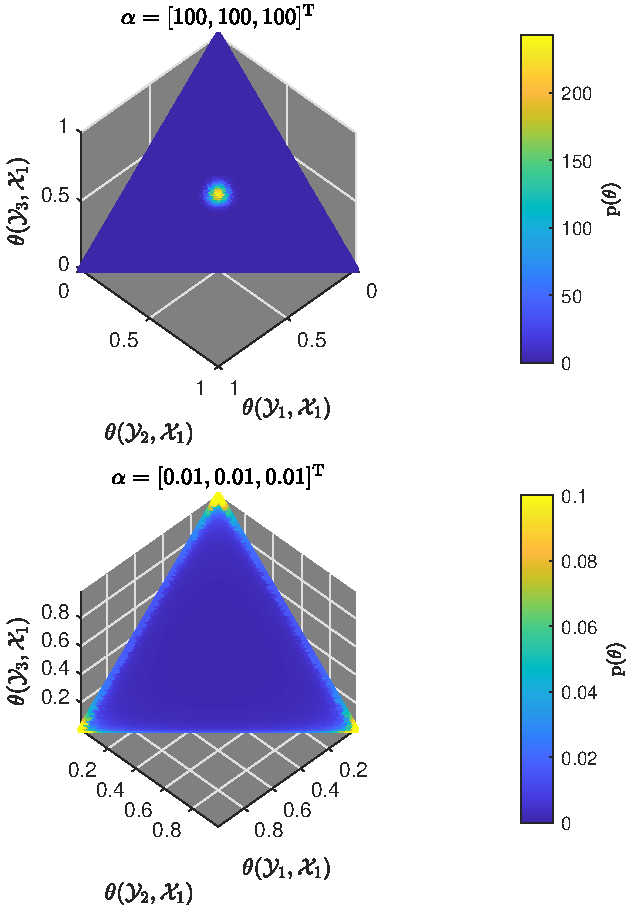
\includegraphics[scale=1.0]{P_theta.pdf}
\caption{Prior distributions for $\bar{\bm{\theta}}$ and $\bm{\theta}$, $M=3$}
\label{fig:P_theta}
\end{figure}



\subsection{Training Set PMF, $\text{P}(\Drm)$}

PGR: graphic examples for DM???

Next, determine the training data PMF, $\text{P}(\Drm)$. The distribution conditioned on the model can be formulated as
\begin{IEEEeqnarray}{rCl}
\text{P}\big( \Drm | \bm{\theta} \big) & = & \prod_{n=1}^N \text{P}\big( \Drm(n) | \bm{\theta} \big) \\
& = & \prod_{y \in \Ycal} \prod_{x \in \Xcal} \bm{\theta}(y,x)^{\bar{N}(y,x;\Drm)} \nonumber \;,
\end{IEEEeqnarray}
where the dependency on the training data $\Drm$ is expressed though a transform functional $\bar{N} : \Dcal \mapsto \bar{\Ncal}$, defined as
\begin{IEEEeqnarray}{rCl}
\bar{N}(\yrm,\xrm;\Drm) & = & \sum_{n=1}^N \delta \big[ (\yrm,\xrm),\Drm(n) \big] \\
& = & \sum_{n=1}^N \delta \left[ \yrm,\Yrm(n) \right] \delta \left[ \xrm,\Xrm(n) \right] \nonumber \;.
\end{IEEEeqnarray}
For a given data set $\Drm$, the function $\bar{\bm{N}}(\Drm)$ over $\Ycal \times \Xcal$ sums to $N$, such that
\begin{IEEEeqnarray}{rCl}
\bar{N}(\cdot,\cdot;\Drm) & \in & \bar{\Ncal}
= \left\{ \bar{\bm{n}} \in \mathbb{N}^{\Ycal \times \Xcal}: \sum_{y \in \Ycal} \sum_{x \in \Xcal} \bar{n}(y,x) = N \right\} \;.
\end{IEEEeqnarray}
The cardinality of this set is $|\bar{\Ncal}| = \binom{N+|\Ycal||\Xcal|-1}{N,|\Ycal||\Xcal|-1}$; note that $|\bar{\Ncal}| \leq |\Dcal|$. 


This transform defines a new random function $\nbarrm(\cdot,\cdot) \equiv \bar{N}(\cdot,\cdot;\Drm)$. Conditioned on the model $\theta$, the PMF of $\nbarrm$ is a multinomial distribution
\begin{IEEEeqnarray}{rCl}
\text{P}(\nbarrm | \bm{\theta}) & = & \sum_{D : \bar{N}(D) = \nbarrm} \text{P}_{\Drm | \theta}(D | \theta) \\
& = & \big|\{ D : \bar{N}(D) = \nbarrm \}\big| \prod_{y \in \Ycal} \prod_{x \in \Xcal} \theta(y,x)^{\bar{\nrm}(y,x)} \nonumber \\
& = & \binom{N}{\nbarrm} \prod_{y \in \Ycal} \prod_{x \in \Xcal} \theta(y,x)^{\bar{\nrm}(y,x)} \nonumber \;,
\end{IEEEeqnarray}
where the binomial coefficient is compactly notated as
\begin{equation}
\binom{N}{\nbarrm} = \frac{N!}{\prod_{y \in \Ycal} \prod_{x \in \Xcal} \bar{\nrm}(y,x)!} \;.
\end{equation}

As the Dirichlet distribution characterizes the parameters of this multinomial distribution, the marginal PMF of $\nbarrm$ is a Dirichlet-Multinomial distribution,
\begin{IEEEeqnarray}{rCl}
\text{P}(\nbarrm) & = & \binom{N}{\nbarrm} \beta(\bm{\alpha})^{-1} \beta(\bm{\alpha} + \nbarrm) \;.
\end{IEEEeqnarray}

PGR: DM reference




Thus, the marginal PMF of the training data is
\begin{IEEEeqnarray}{rCl}
\text{P}(\Drm) & = & \text{E}_{\bm{\theta}} \left[ \prod_{n=1}^N \text{P}\big( \Drm(n) | \bm{\theta} \big) \right] \\
& = & \text{E}_{\bm{\theta}} \left[ \prod_{y \in \Ycal} \prod_{x \in \Xcal} \bm{\theta}(y,x)^{\bar{N}(y,x;\Drm)} \right] \nonumber \\
& = & \beta(\bm{\alpha})^{-1} \beta \left(  \bm{\alpha} + \bar{\bm{N}}(\Drm) \right) \nonumber \;.
\end{IEEEeqnarray}
This perspective shows values of the PMF $\text{P}(\Drm)$ to be joint moments of the model $\theta$. 



The first and second joint moments of $\bar{\nrm}$ are
\begin{IEEEeqnarray}{rCl}
\mu_{\bar{\nrm}}(y,x) & = & \text{E}[\bar{\nrm}(y,x)] \\
& = & N \frac{\alpha(y,x)}{\alpha_0} = N \mu_\theta(y,x) \nonumber
\end{IEEEeqnarray}
and
\begin{IEEEeqnarray}{L}
\text{E}\big[ \bar{\nrm}(y,x) \bar{\nrm}(y',x') \big] \\
= \frac{N}{\alpha_0 (\alpha_0+1)} \big( (\alpha_0 + N)\alpha(y,x) \delta[y,y'] \delta[x,x'] + (N-1) \alpha(y,x) \alpha(y',x') \big) \nonumber \;.
\end{IEEEeqnarray}
The covariance function is
\begin{IEEEeqnarray}{L}
\text{E}\Big[ \big( \bar{\nrm}(y,x) - \mu_{\bar{\nrm}}(y,x) \big) \big( \bar{\nrm}(y',x') - \mu_{\bar{\nrm}}(y',x') \big) \Big] \\
\quad = \frac{N (\alpha_0+N)}{\alpha_0+1} \big( \mu_\theta(y,x) \delta[y,y'] \delta[x,x'] - \mu_\theta(y,x) \mu_\theta(y',x') \big) \nonumber
\end{IEEEeqnarray}



PGR: CHECK/PROVE THE FOLLOWING???

For $\alpha_0 \to \infty$, the PDF concentrates at its mean, resulting in
\begin{IEEEeqnarray}{rCl}
\text{P}(\nbarrm) & = & \binom{N}{\nbarrm} \prod_{y \in \Ycal} \prod_{x \in \Xcal} \left(\frac{\alpha(y,x)}{\alpha_0}\right)^{\bar{\nrm}(y,x)} \\
& = & \binom{N}{\nbarrm} \alpha_0^{-N} \prod_{y \in \Ycal} \prod_{x \in \Xcal} \alpha(y,x)^{\bar{\nrm}(y,x)} \nonumber \;.
\end{IEEEeqnarray}
Conversely, for $\alpha_0 \to 0$, the PDF trends toward
\begin{IEEEeqnarray}{rCl}
\text{P}(\nbarrm) & = & \sum_{y \in \Ycal} \sum_{x \in \Xcal} \frac{\alpha(y,x)}{\alpha_0} \delta\big[ \nbarrm , N \bm{e}(y,x) \big] \\
& = & \sum_{y \in \Ycal} \sum_{x \in \Xcal} \frac{\alpha(y,x)}{\alpha_0} \prod_{y' \in \Ycal} \prod_{x' \in \Xcal} \delta \big[ \bar{\nrm}(y',x') , N \delta[y,y'] \delta[x,x'] \big] \nonumber \;.
\end{IEEEeqnarray}

\begin{IEEEeqnarray}{rCl}
\text{P}(\Drm) & = & \sum_{y \in \Ycal} \sum_{x \in \Xcal} \frac{\alpha(y,x)}{\alpha_0} \prod_{n=1}^N \delta\big[ (y,x),\Drm(n) \big] \;.
\end{IEEEeqnarray}



PGR: Uniform


Finally, we extend the representation for the PMF to
\begin{IEEEeqnarray}{rCl} \label{P_D_io}
\text{P}(\Drm) & = & \binom{N+M-1}{\ldots,\bar{N}(y,x;\Drm),\ldots,M-1}^{-1} \\
& = & \binom{N+M-1}{N,M-1}^{-1} \binom{N}{\ldots,\bar{N}(y,x;\Drm),\ldots}^{-1} \nonumber\;.
\end{IEEEeqnarray}
Again, the probability of a specific training set is dependent on the data through the multinomial coefficient of transform $\bar{\bm{N}}(\Drm)$.

PGR: use multinomial operator to eliminate set indexing

PGR: concentration talk: differs between D and nbar? with alpha and with N? Graphics? 









\subsection{Conditonal PMF $\text{P}(\yrm | \xrm,\Drm)$}

As shown in Equation \eqref{eq:f_opt_xD}, the decision selected by the optimally designed function depend on $\text{P}(\yrm | \xrm,\Drm)$, the distribution of the unobserved $\yrm$ conditioned on all observable random variables.

To determine this distribution, first observe that the model posterior PDF given the training data is
\begin{IEEEeqnarray}{rCl}
\text{p}(\bm{\theta} | \Drm) & = & \frac{\text{P}(\Drm | \bm{\theta}) \text{p}(\bm{\theta})}{\text{P}(\Drm)} \\
& = & \beta \left( \bm{\alpha} + \bar{\bm{N}}(\Drm) \right)^{-1} \prod_{y \in \Ycal} \prod_{x \in \Xcal} 
\theta(y,x)^{\alpha(y,x) + \bar{N}(y,x;\Drm) - 1} \;, \nonumber
\end{IEEEeqnarray}
a Dirichlet distribution with parameter function $\alpha + \bar{N}(\cdot,\cdot;\Drm)$. 

This posterior distribution is of specific interest in the machine learning literature. While Bayesian techniques are used here, often point estimates of the model $\theta$ are formed; perhaps the most common approach is to form the Maximum a posteriori estimate,
\begin{IEEEeqnarray}{rCl}
\theta_\text{MAP}(\Drm) & = & \argmax_{\theta \in \Theta} \text{P}(\theta|\Drm) = \frac{\bar{\bm{N}}(\Drm)}{N} \;,
\end{IEEEeqnarray}
which is simply the empirical distribution. 

PGR: ML equal MAP for uniform comment?

Also, as the concentration parameter increases proportionately with increasing volumes of training data, as $N \to \infty$ the posterior converges to $\text{p}(\theta | \Drm) \to \bar{\bm{N}}(\Drm) / N$. Thus, as more data is collected, the model can be more positively identified and used to formulate minimum risk decisions.

PGR: reference Dir convergence in prev section

\begin{figure}
\centering
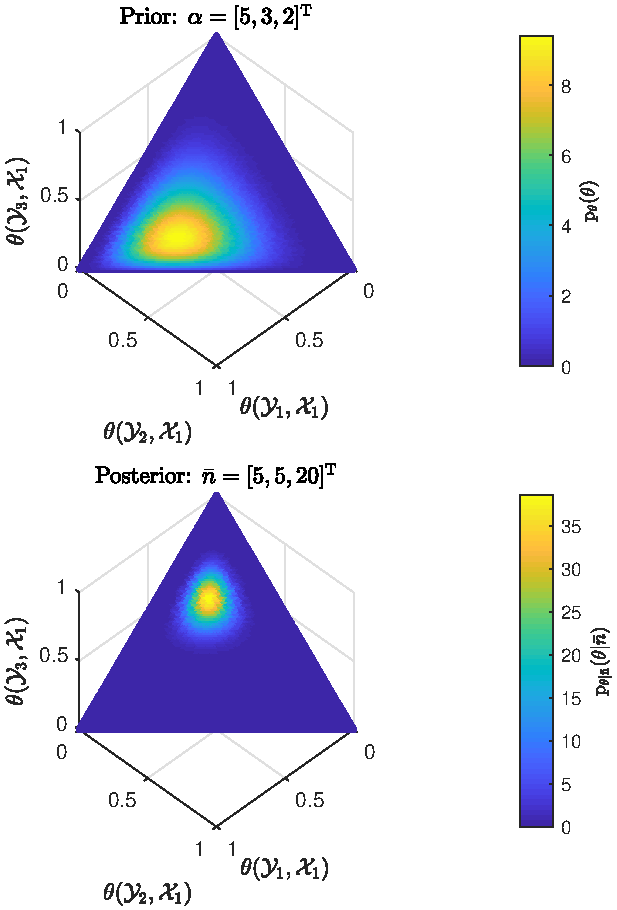
\includegraphics[scale=1.0]{P_theta_post.pdf}
\caption{Posterior model PDF's for various training sets $D$}
\label{fig:P_theta_D}
\end{figure}

PGR: before/after sharpening graphic???



Next the joint PMF of $\yrm$ and $\xrm$ conditioned on the training data is expressed as
\begin{IEEEeqnarray}{rCl}
\text{P}(\yrm,\xrm|\Drm) & = & \frac{\text{E}_{\bm{\theta}}\big[ \theta(\yrm,\xrm) \text{P}(\Drm | \theta) \big]}{\text{P}(\Drm)}  \\
& = & \text{E}_{\bm{\theta} | \Drm}\big[ \theta(\yrm,\xrm) | \Drm \big] \nonumber \\
& = & \frac{\alpha(\yrm,\xrm) + \bar{N}(\yrm,\xrm;\Drm)}{\alpha_0 + N} \nonumber \;.
\end{IEEEeqnarray}

Finally, the distribution of interest is generated via Bayes rule as
\begin{IEEEeqnarray}{rCl}
\text{P}(\yrm | \xrm,\Drm) & = & \frac{\text{P}(\yrm,\xrm | \Drm)}{\text{P}(\xrm | \Drm)} \\
& = & \frac{\alpha(\yrm,\xrm) + \bar{N}(\yrm,\xrm;\Drm)}{\alpha'(\xrm) + N'(\xrm;\Drm)} \nonumber \\
& = & \left(\frac{\alpha'(\xrm)}{\alpha'(\xrm) + N'(\xrm;\Drm)}\right) \frac{\alpha(\yrm,\xrm)}{\alpha'(\xrm)} \nonumber \\
&& \quad + \left(\frac{N'(\xrm;\Drm)}{\alpha'(\xrm) + N'(\xrm;\Drm)}\right) \frac{\bar{N}(\yrm,\xrm;\Drm)}{N'(\xrm;\Drm)} \nonumber \;,
\end{IEEEeqnarray}
where we introduce ``marginalized'' functions $\alpha'(x) = \sum_{y \in \Ycal} \alpha(y,x)$ and $N'(x;\Drm) = \sum_{y \in \Ycal} \bar{N}(y,x;\Drm) = \sum_{n=1}^N \delta\big[ x,\Xrm(n) \big]$. 

The last representation views the distribution as a convex combination of two conditional distributions. The first distribution $\text{P}(\yrm | \xrm) = \text{E}_{\theta}\big[ \theta(\yrm,\xrm) \big] / \text{E}_{\theta}\big[ \theta'(\xrm) \big] = \alpha(\yrm,\xrm) / \alpha'(\xrm)$ is independent of the training data and based on the prior knowledge implied via the model PDF parameter; the second distribution is a ``conditional'' empirical PMF and depends on $\Drm$, not on $\alpha$. For both, only those values $\alpha$ and $\Drm$ corresponding to the observed value $\xrm$ shape the distribution. 

Similarly, the weighting factors are only influenced by these values. As the number of training examples increases or as $\alpha_0 \to 0$, $\text{P}(\yrm | \xrm,\Drm)$ trends towards the empirical distribution; for $N'(\xrm;\Drm) = 0$ or as $\alpha_0 \to \infty$, the PMF trends toward the prior distribution $\text{P}(\yrm|\xrm)$.

PGR: divide by zero comment?

PGR: theta marginal?



Athough the distribution of interest has already been expressed, it is informative to introduce a different representation,
\begin{IEEEeqnarray}{rCl}
\text{P}(\yrm | \xrm,\Drm) & = & \text{E}_{\bm{\theta} | \xrm,\Drm} \big[ \text{P}(\yrm | \xrm,\bm{\theta}) \big] \\
& = & \text{E}_{\bm{\theta} | \xrm,\Drm} \left[ \frac{\theta(\yrm,\xrm)}{\sum_{y' \in \Ycal} \theta(y',\xrm)} \right] \nonumber \;.
\end{IEEEeqnarray}
Just as $\text{P}(\yrm,\xrm | \Drm)$ is an expectation of $\theta$ using a PDF conditioned on $\Drm$, $\text{P}(\yrm | \xrm,\Drm)$ is an expectation based on the model posterior conditioned on both observed random variables. The expectation operates on a function of $\theta$ where each portion of the function $\theta(\cdot,\xrm)$ is normalized. 

The complete model posterior PDF is represented as
\begin{IEEEeqnarray}{rCl}
\text{p}(\bm{\theta} | \xrm, \Drm) & = & \frac{\text{P}(\xrm | \bm{\theta}) \text{p}(\bm{\theta} | \Drm)}{\text{P}(\xrm | \Drm)} = \text{E}_{\yrm | \xrm,\Drm} \big[ \text{p}(\bm{\theta} | \yrm,\xrm,\Drm) \big] \\
& = & \sum_{y' \in \Ycal} \frac{\alpha(y',\xrm) + \bar{N}(y',\xrm;\Drm)}{\alpha'(\xrm) + N'(\xrm;\Drm)} \text{Dir}\bigg( \bm{\theta} ; \bm{\alpha} + \bar{\bm{N}}\Big( \big( (y',\xrm),\Drm \big) \Big) \bigg) \nonumber \;.
\end{IEEEeqnarray}
This is a mixture distribution. The weighting factors are, interestingly, the values of $\text{P}(\yrm | \xrm,\Drm)$ given the observations. The PDF's being combined are Dirichlet distributions with different parameterizing functions $\alpha(y,x) + \bar{N}\Big( y,x;\big( (y',\xrm),\Drm \big) \Big) = \alpha(y,x) + \bar{N}(y,x;\Drm) + \delta[y,y'] \delta[x,\xrm]$; additional emphasis is put on the $M_y$ different possible pairs $(y,x)$ including the observed value $\xrm$.

To confirm that the expectation produces the same distribution $\text{P}(\yrm | \xrm,\Drm)$ displayed previously, use the distribution of a Dirichlet random function conditioned on its aggregation, proven in Appendix \ref{app:Dir_agg}, to show $\text{E}_{\theta}\big[ \theta(y,x) / \theta'(x) \big] = \alpha(y,x) / \alpha'(x)$. The PMF is evaulated as
\begin{IEEEeqnarray}{rCl}
\text{P}(\yrm | \xrm,\Drm) & = & \sum_{y' \in \Ycal} \frac{\alpha(y',\xrm) + \bar{N}(y',\xrm;\Drm)}{\alpha'(\xrm) + N'(\xrm;\Drm)} \left( \frac{\alpha(\yrm,\xrm) + \bar{N}(\yrm,\xrm;\Drm) + \delta[y',\yrm] \delta[\xrm,\xrm]}{\alpha'(\xrm) + N'(\xrm;\Drm) + \delta[\xrm,\xrm]} \right) \\
& = & \frac{\alpha(\yrm,\xrm) + \bar{N}(\yrm,\xrm;\Drm)}{\alpha'(\xrm) + N'(\xrm;\Drm)} \nonumber \;.
\end{IEEEeqnarray}







PGR: UNIFORM


\begin{IEEEeqnarray}{rCl} \label{P_y_xD_basic}
\text{P}(\yrm | \xrm,\Drm) & = & \frac{\bar{N}(\yrm,\xrm;\Drm)+1}{N'(\xrm;\Drm) + M_y} \\
& = & \left( \frac{M_y}{N'(\xrm;\Drm) + M_y} \right) \frac{1}{M_y} + \nonumber \\
&& \quad \left( \frac{N'(\xrm;\Drm)}{N'(\xrm;\Drm) + M_y} \right) \frac{\bar{N}(\yrm,\xrm;\Drm)}{N'(\xrm;\Drm)} \nonumber \;.
\end{IEEEeqnarray}

Again, we have a convex combination of two PMF's: a uniform distribution over the $M_y$ possible outputs, and an empirical conditional distribution. This is a notable difference from the basic model; now, each decision is only informed by training samples having the same input value $\xrm$. Thus, for a specific input $\xrm$, the conditional distribution will ``sharpen'' to a degree proportionate to the marginal PMF, $\text{P}(\xrm | \bm{\theta})$, which can be approximated by $N'(\xrm;\Drm)/N$.

PGR: accurate statement?

PGR: use the math to express PyxD???







\newpage





\section{Applications: General uniform MAIN}

In this section, loss functions typical for classification and regression applications, specifically the 0-1 loss function and the squared-error loss function, are adopted. Optimal learners $f^*(\xrm;\Drm)$ are found and the corresponding minimum risk $\Rcal(f^*)$ is assessed.

As shown in Equation \eqref{eq:f_opt_xD}, the decision expressed for a given input $\xrm$ and training set $\Drm$ minimizes the metric
\begin{IEEEeqnarray}{L} \label{eq:E_y|xD L}
\text{E}_{\yrm | \xrm,\Drm} \big[ \mathcal{L}(h,\yrm) \big] = \sum_{y \in \Ycal} \mathcal{L}(h,y) \text{P}_{\yrm | \xrm,\Drm}(y | \xrm,\Drm) \\
= \frac{\sum_{y \in \Ycal} \alpha(y,\xrm) \mathcal{L}(h,y) + \sum_{y \in \Ycal} \bar{N}(y,\xrm;\Drm) \mathcal{L}(h,y)}{\alpha'(\xrm) + N'(\xrm;\Drm)} \nonumber \\
= \left(\frac{\alpha'(\xrm)}{\alpha'(\xrm) + N'(\xrm;\Drm)}\right) \sum_{y \in \Ycal} \frac{\alpha(y,\xrm)}{\alpha'(\xrm)} \mathcal{L}(h,y) + \left(\frac{N'(\xrm;\Drm)}{\alpha'(\xrm) + N'(\xrm;\Drm)}\right) \sum_{y \in \Ycal} \frac{\bar{N}(y,\xrm;\Drm)}{N} \mathcal{L}(h,y) \nonumber \\
= \left(\frac{\alpha'(\xrm)}{\alpha'(\xrm) + N'(\xrm;\Drm)}\right) \text{E}_{\yrm | \xrm}\big[ \mathcal{L}(h,\yrm) \big] + \left(\frac{N'(\xrm;\Drm)}{\alpha'(\xrm) + N'(\xrm;\Drm)}\right) \frac{\sum_{n=1}^N \delta\big[ \xrm,\Xrm(n) \big] \mathcal{L}\big( h,\Yrm(n) \big)}{\sum_{n=1}^N \delta\big[ \xrm,\Xrm(n) \big]} \nonumber \;.
\end{IEEEeqnarray}

The expectation can be represented as a convex combination of two expected losses. The first expected loss is evaluated with respect to the conditional distribution $\text{P}(\yrm|\xrm)$, which reflects the prior knowledge encapsulated in model parameter $\alpha$. The second term is a conditional emprical loss, or the average loss among samples $\Yrm(n)$ whose corresponding values $\Xrm(n)$ match the observed value $\xrm$.



\subsection{0-1 Loss}

In this section, we will apply the developed framework to the machine learning problem to which it is most applicable: classification. In classification problems, the unobserved variable space is countable and typically finite. Furthermore, the hypothesis space  is usually identical to the unobserved variable space, that is $\Hcal = \Ycal$. The 0-1 loss function is the most well known for these problems; it is represented as
\begin{equation} \label{loss_01}
\mathcal{L}(h,y) = 1 - \delta[h,y] \;.
\end{equation}

Applying this loss function, the conditional risk \eqref{eq:risk_cond} is
\begin{IEEEeqnarray}{rCl}
\mathcal{R}_{\Theta}(f | \theta) & = & 1 -  \text{E}_{\Drm | \bm{\theta}} \bigg[ \text{E}_{\yrm,\xrm | \bm{\theta}} \Big[ \delta\big[ f(\xrm,\Drm),\yrm \big] \Big] \bigg] \\
& = & 1 -  \sum_{x \in \Xcal} \text{E}_{\Drm | \bm{\theta}} \Big[ \theta\big( f(x,\Drm),x \big) \Big] \nonumber \;.
\end{IEEEeqnarray}
Evaluated with a Dirichlet prior, the full risk is
\begin{IEEEeqnarray}{rCl} \label{eq:risk_01}
\mathcal{R}(f) & = & 1 - \text{E}_{\bm{\theta}} \left[ \sum_{x \in \Xcal} \text{E}_{\Drm | \bm{\theta}} \Big[ \theta\big( f(x,\Drm),x \big) \Big] \right] \\
& = & 1 - \sum_{x \in \Xcal} \frac{\text{E}_{\Drm} \Big[ \alpha\big( f(x,\Drm),x \big) + \bar{N}\big( f(x,\Drm),x ; \Drm \big) \Big]}{\alpha_0 + N} \nonumber \\
& = & 1 - \sum_{x \in \Xcal} \frac{\text{E}_{\nbarrm} \Big[ \alpha\big( f(x,\nbarrm),x \big) + \bar{\nrm}\big( f(x,\nbarrm),x \big) \Big]}{\alpha_0 + N} \nonumber \;.
\end{IEEEeqnarray}



\subsubsection{Optimal Learner: Conditional MAP}

To determine the optimal learning function, substitute the 0-1 loss from Equation \eqref{loss_01} into Equation \eqref{eq:E_y|xD L} and Equation \eqref{eq:f_opt_xD} to find
\begin{IEEEeqnarray}{rCl} \label{eq:f_opt_01}
f^*(\xrm,\Drm) & = & \argmin_{h \in \Ycal} \frac{\sum_{y \in \Ycal} \big( \alpha(y,\xrm) + \bar{N}(y,\xrm;\Drm) \big) \big( 1 - \delta[h,y] \big)}{\alpha'(\xrm) + N'(\xrm;\Drm)} \\
& = & \argmax_{h \in \Ycal} \text{P}_{\yrm | \xrm,\Drm}(h | \xrm,\Drm) \nonumber \\
& = & \argmax_{y \in \Ycal} \left( \alpha(y,\xrm) + \bar{N}(y,\xrm;\Drm) \right) \nonumber \;.
\end{IEEEeqnarray}
The optimal classifier chooses the value $\yrm$ that has the maximum value in the conditional PMF for the observed value of $\xrm$; each candidate decision $h \in \Ycal$ is scored by counting the number of training samples that occur with the same observed value as $\xrm$ and weighting with the prior knowledge imparted by $\alpha$.


PGR: UNIFORM

When the uniform prior is used, the decision becomes 
\begin{IEEEeqnarray}{rCl}
f^*(\xrm,\Drm) & = & \argmax_{y \in \Ycal} \bar{N}(y,\xrm;\Drm) \;,
\end{IEEEeqnarray}
a majority decision which simply chooses the class from $\Ycal$ most often found among training set samples $\Drm$ with a matching input value $\xrm$. This is intuitive, as the model PDF provides no confidence as to which classes may be most likely.


\subsubsection{Minimum Risk: Probability of Error}

Substituting the optimal learner \eqref{eq:f_opt_01} into the general risk \eqref{eq:risk_01}, the minimum probability of error is 
\begin{IEEEeqnarray}{rCl}
\mathcal{R}(f^*) & = & 1 - \text{E}_{\xrm,\Drm} \left[ \max_{y \in \Ycal} \text{P}_{\yrm | \xrm,\Drm}(y | \xrm,\Drm) \right] \\
& = & 1 - \sum_{x \in \Xcal} \frac{\text{E}_{\nbarrm} \Big[ \max_{y \in \Ycal} \big( \alpha(y,x) + \bar{\nrm}(y,x) \big) \Big]}{\alpha_0 + N} \nonumber \;.
\end{IEEEeqnarray}

PGR: missing info for Dir gen graphics? fixed y given x conditional alpha???

PGR: no closed-forms found???


\begin{figure}
\centering
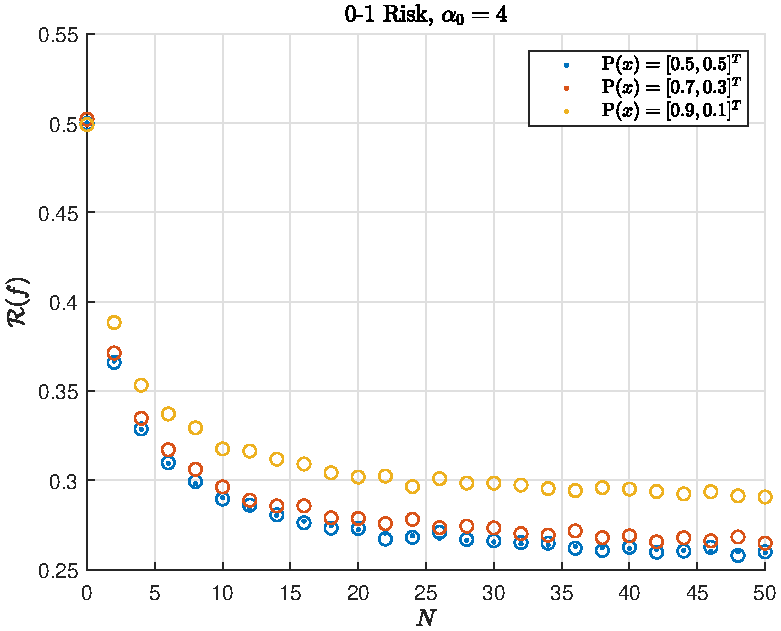
\includegraphics[scale=1.0]{Risk_01_Dir_IO_N_leg_Px.pdf}
\caption{Optimal 0-1 Risk vs $N$}
\label{fig:Risk_01_Dir_IO_N_leg_Px}
\end{figure}

\begin{figure}
\centering
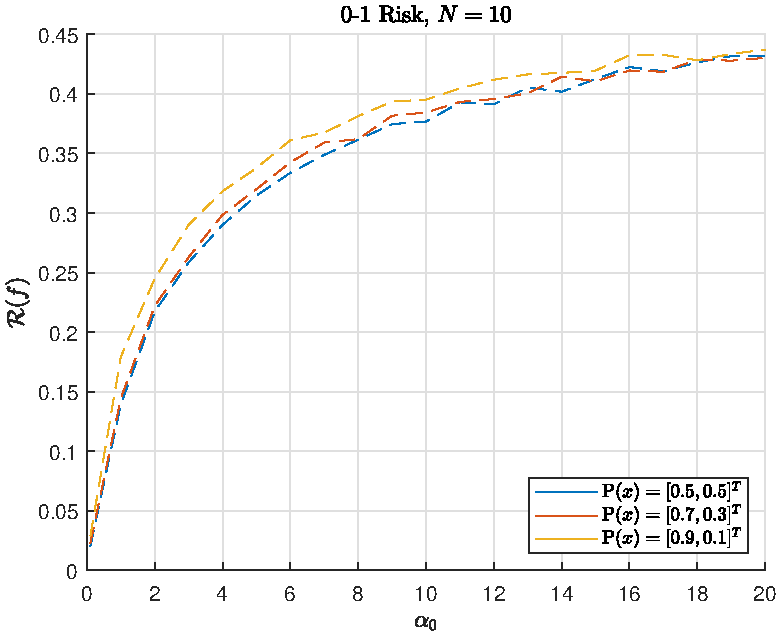
\includegraphics[scale=1.0]{Risk_01_Dir_IO_a0_leg_Px.pdf}
\caption{Optimal 0-1 Risk vs $\alpha_0$}
\label{fig:Risk_01_Dir_IO_a0_leg_Px}
\end{figure}

\begin{figure}
\centering
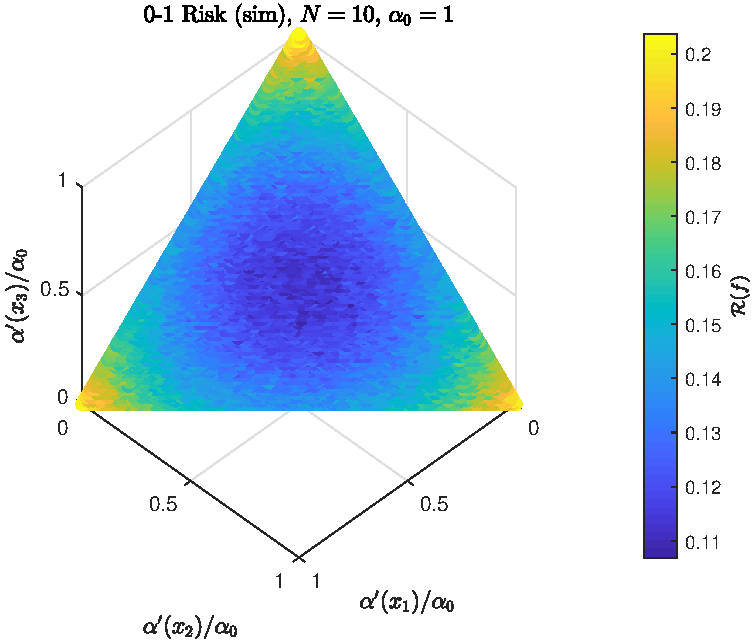
\includegraphics[scale=1.0]{Risk_01_Dir_IO_Px_N_10_a0_1.pdf}
\caption{Optimal 0-1 Risk vs $\text{P}(x)$}
\label{fig:Risk_01_Dir_IO_Px_N_10_a0_1}
\end{figure}



PGR: UNIFORM

PGR: Can uniform optimal risk be approximated as a function of My and Mx/N, as is for SE loss???

To assess the minimum risk under the general model, we start from equation \eqref{risk_min_IO} and rework the formula to depend on an expectation over $\text{P}(\Drm)$ as performed orginally, resulting in
\begin{IEEEeqnarray}{rCl}
\mathcal{R}(f^*) & = & \text{E}_{\xrm,\Drm} \bigg[ \text{E}_{\yrm | \xrm,\Drm} \Big[ \mathcal{L}\big( f^*(\xrm,\Drm),\yrm \big) \Big] \bigg] \\
& = & 1 - \text{E}_{\xrm,\Drm} \left[ \max_{y} \text{P}_{\yrm | \xrm,\Drm}(y | \xrm,\Drm) \right] \nonumber \\
& = & 1 - \sum_{x \in \Xcal} \text{E}_{\Drm} \left[ \max_{y} \text{P}_{\yrm,\xrm | \Drm}(y,x | \Drm) \right] \nonumber \\
& = & 1 - \frac{\sum_{x \in \Xcal} \text{E}_{\Drm} \left[\max_{y} \bar{N}(y,x;\Drm) \right] + 1}{N+M} \nonumber \;.
\end{IEEEeqnarray}

Now, however, the argument of expectation is the maximum of a subset of $\bar{\bm{N}}(\Drm)$, $M_y$ out of $M_xM_y$, rather than the entire random variable. As shown in Appendix \ref{app:E_N_bar}, all marginal distributions of $\nbarrm$ have the same form; as such, the expectations will be the same regardless of which $M_y$ variables the maximum operator is applied to. 

To evaluate the expectation for an abritrary value $x$, we find a formula for the CMF of the maximum of any $k$ of $M$ entries of random matrix $\nbarrm$. Introduce subset $\Ycal' \subset \Ycal$ with cardinality $k$. Denote the new variable as $\bar{\nrm}_{\text{max}}^k \equiv \max_{y \in \Ycal'} \bar{\nrm}(y)$; we find in Appendix ??? that the CMF is equivalent to
\begin{IEEEeqnarray}{rCl}
F_{\bar{\nrm}_{\text{max}}^k}(n) & = & \text{P}\big( \bar{\nrm}_{\text{max}}^k \leq n \big) \\
& = & \sum_{m=0}^k \binom{k}{m} (-1)^m \prod_{l=1}^{M-1} \left( 1 - \frac{m(n+1)}{N+l} \right) \nonumber \\
&& \quad  \left[ U(n) - U\left( n+1- \left\lceil \frac{N+M}{m} \right\rceil \right) \right] \nonumber \;.
\end{IEEEeqnarray}
Evaluating the expectation, we have
\begin{IEEEeqnarray}{rCl}
\text{E}_{\bar{\bm{n}}} \left[ \bar{\nrm}_{\text{max}}^k \right] & = & N+M - \sum_{n=0}^{N+M-1} F_{\bar{\nrm}_{\text{max}}^k}(n) \\
& = & - \sum_{m=1}^k \binom{k}{m} (-1)^m \left[ \sum_{n=1}^{N+M} \prod_{l=1}^{M-1} \left( 1 - \frac{mn}{N+l} \right) - \sum_{n=\left\lceil \frac{N+M}{m} \right\rceil}^{N+M} \prod_{l=1}^{M-1} \left( 1 - \frac{mn}{N+l} \right) \right] \nonumber \;.
%& = & sumbounds??? - \sum_{m=1}^k \binom{k}{m} (-1)^m \sum_{n=1}^{\left\lceil \frac{N+M}{m} \right\rceil -1} \prod_{l=1}^{M-1} \left( 1 - \frac{mn}{N+l} \right) \;.
\end{IEEEeqnarray}
Making use of the summation identity
\begin{equation}
\sum_{m=0}^k \binom{k}{m} (-1)^m = 0 \;,
\end{equation}
we substitute in to the formula for minimum risk using $k=M_y$, resulting in
\begin{IEEEeqnarray}{rCl}
\mathcal{R}(f^*) & = & 1 + \frac{M_x}{N+M} \sum_{m=1}^{M_y} \binom{M_y}{m} (-1)^m \sum_{n=0}^{\left\lceil \frac{N+M}{m} \right\rceil -1} \prod_{l=1}^{M-1} \left( 1 - \frac{mn}{N+l} \right) \;.
\end{IEEEeqnarray}

PGR: Proof? CHECK....???



Figure \ref{fig:Risk_01_IO_N} displays how the optimal risk decreases with increasing training data; the number of outputs is fixed at $M_y = 2$ and multiple series are provided for different input set sizes $M_x$. The plot for $M_x = 1$ is obviously identical to the series shown in Section \ref{sec:uniform_basic_apps_01}. For larger input set sizes, the risk is still $\mathcal{R}(f^*) = 0.5$ when $N = 0$, but the rate of decrease with $N$ suffers. 

\begin{figure}
\centering
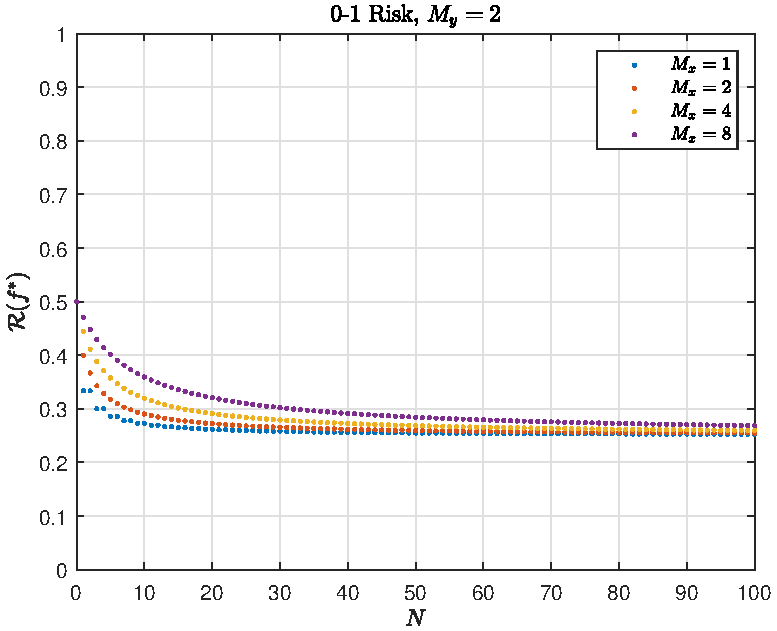
\includegraphics[scale=1.0]{Risk_01_IO_N.pdf}
\caption{Optimal 0-1 Risk vs training set size for various input set sizes}
\label{fig:Risk_01_IO_N}
\end{figure}

Further insight into how $M_x$ affects the risk can be acquired by plotting the risk vs $N/M_x$. In Figure \ref{fig:Risk_01_IO_N-Mx}, it is shown that the optimal risk can be approximated by a function dependent only on $N/M_x$; of the series plotted, only the series for $M_x = 1$ shows notable deviation from the others.

\begin{figure}
\centering
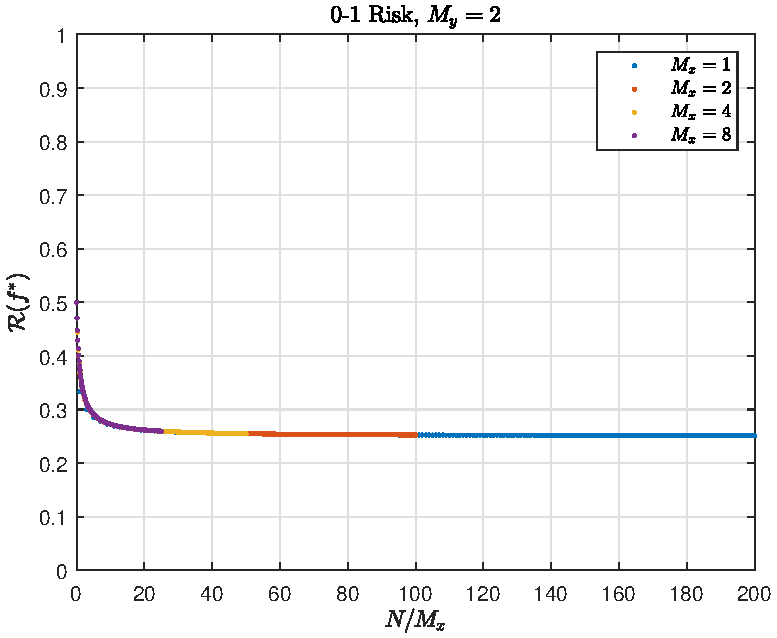
\includegraphics[scale=1.0]{Risk_01_IO_N-Mx.pdf}
\caption{Optimal 0-1 Risk vs training set size for various input set sizes}
\label{fig:Risk_01_IO_N-Mx}
\end{figure}



As for the basic model, it is informative to note how the minimum risk trends with increasing volume of training data. Noting that
\begin{IEEEeqnarray}{rCl}
\lim_{N \to \infty} (N+M)^{-1} \sum_{n=0}^{\left\lceil \frac{N+M}{m} \right\rceil -1} \prod_{l=1}^{M-1} \left( 1 - \frac{mn}{N+l} \right) & = & \\
\lim_{N/m \to \infty} m^{-1} \frac{m}{N} \sum_{n=0}^{\left\lceil \frac{N}{m} \right\rceil -1} \left( 1 - \frac{mn}{N} \right)^{M-1} & = & \nonumber \\
m^{-1} \int_0^1 (1-t)^{M-1} \mathrm{d} t & = & \frac{1}{mM} \nonumber \;,
\end{IEEEeqnarray}
and using the same concepts from Appendix \ref{app:E_N_max}, we find
\begin{IEEEeqnarray}{rCl}
\mathcal{R}(f^*) & = & 1 + \frac{M_x}{M} \sum_{m=1}^{M_y} \binom{M_y}{m} (-1)^m m^{-1} \\
& = & 1 - \frac{1}{M_y} \sum_{m=1}^{M_y} \frac{1}{m} \nonumber \;.
\end{IEEEeqnarray}

%\begin{IEEEeqnarray}{rCl}
%1 - \mathcal{R}(f^*) & = & -\frac{M_x}{M} \sum_{m=1}^{M_y} \binom{M_y}{m} (-1)^m m^{-1} \\
%& = & \frac{1}{M_y} \sum_{m=1}^{M_y} \frac{1}{m} \;.
%\end{IEEEeqnarray}

Again, we have a harmonic number dependent on the number of possible outputs $M_y$. With infinite training data, there will be an infinite number of samples for each possible input $\xrm$; as a result, there is no loss of classification performance regardless of the input dimension $M_x$. This agrees with the notion that optimal 0-1 risk can be approximated as a function of $N/M_x$.







\subsection{Squared-Error Loss}

\subsubsection{Optimal Learner: The Posterior Mean}

For the squared-error loss function, the optimal decison function generalizes to the expected value of $\yrm$, conditioned on the observed value $\xrm$ as well as on the training data $\Drm$ (i.e. all observable variables). Extending from the basic model, we have $\yrm$ and $\xrm$ take on numerical values such that $\Ycal = \{1,\ldots,M_y\}$ and $\Xcal = \{1,\ldots,M_x\}$. The optimal learner is the posterior mean,
\begin{IEEEeqnarray}{rCl}
f^*(\xrm,\Drm) & = & \argmin_{h \in \mathbb{R}} \text{E}_{\yrm | \xrm,\Drm} \left[ (h-\yrm)^2 \right] \\
& = & \sum_{y=1}^{M_y} y \text{P}_{\yrm | \xrm,\Drm}(y | \xrm, \Drm) \equiv \mu_{\yrm | \xrm,\Drm}(\xrm, \Drm) \nonumber \\
& = & \left( \frac{M_y}{N'(\xrm;\Drm) + M_y} \right) \frac{M_y+1}{2} + \nonumber \\
&& \quad \left( \frac{N'(\xrm;\Drm)}{N'(\xrm;\Drm) + M_y} \right) \sum_{y=1}^{M_y} y \frac{\bar{N}(y,\xrm;D)}{N'(\xrm;\Drm)} \nonumber \\
& = & \left( \frac{M_y}{N'(\xrm;\Drm) + M_y} \right) \frac{M_y+1}{2} + \nonumber \\
&& \quad \left( \frac{N'(\xrm;\Drm)}{N'(\xrm;\Drm) + M_y} \right) \frac{\sum_{n=1}^N \delta\big[ \xrm,\Xrm(n) \big] \Yrm(n)}{N'(\xrm;\Drm)} \nonumber \;.
\end{IEEEeqnarray}

Again, we have a convex combination of two conditional means. Now, the weighting factors depend on the cardinality $M_y$ and the number of training data with inputs matching the currently observed value of $\xrm$, $N'(\xrm;\Drm)$.



\subsubsection{Minimum Risk: Expected Posterior Variance}

Under the general model, the optimal learning function is the expected value $\yrm$ additionaly conditioned on the observed variable $\xrm$; similarly, the minimum risk is the expected value of the variance over $\text{P}(\yrm | \xrm,\Drm)$,
\begin{IEEEeqnarray}{rCl}
\mathcal{R}(f^*) & = & \text{E}_{\xrm,\Drm} \bigg[ \text{E}_{\yrm | \xrm,\Drm} \Big[ \mathcal{L}\big( f^*(\xrm,\Drm),\yrm \big) \Big] \bigg] \\
& = &  \text{E}_{\xrm,\Drm} \left[ \Sigma_{\yrm | \xrm,\Drm} \right] = \text{E}_{\xrm,\Drm} \Big[ \text{E}_{\yrm | \xrm,\Drm} \big[ (\yrm - \mu_{\yrm | \xrm,\Drm})^2 \big] \Big] \nonumber \\
& = & \text{E}_{\xrm,\nbarrm} \left[ \Sigma_{\yrm | \xrm,\nbarrm} \right] = \text{E}_{\xrm,\nbarrm} \left[ \text{E}_{\yrm | \xrm,\nbarrm}[\yrm^2] - \left( \text{E}_{\yrm | \xrm,\nbarrm}[\yrm] \right)^2 \right] \nonumber \;.
\end{IEEEeqnarray}

We will assess two expectations over the observables separately. First, we have
\begin{IEEEeqnarray}{rCl}
\text{E}_{\xrm,\nbarrm} \left[ \text{E}_{\yrm | \xrm,\nbarrm}[\yrm^2] \right] & = & \text{E}_{\yrm}[\yrm^2] \\
& = & \sum_{y=1}^{M_y} y^2 M_y^{-1} \nonumber \\
& = & \frac{1}{6}(M_y+1)(2M_y+1) \nonumber \;,
\end{IEEEeqnarray}
where have used $\text{P}(\yrm) = 1/M_y$.

%\begin{IEEEeqnarray}{C}
%\text{E}_{\xrm,\nbarrm} \left[ \left( \text{E}_{\yrm | \xrm,\nbarrm}[\yrm] \right)^2 \right] =
%\sum_{\bar{\bm{n}} \in \bar{\Ncal}} \sum_{m_x=1}^{M_x} \text{P}(x_{m_x},\bar{\bm{n}}) \left( \sum_{m_y=1}^{M_y} m_y \text{P}(y_{m_y} | x_{m_x},\bar{\bm{n}}) \right)^2 \\
%= \sum_{m_x=1}^{M_x} \sum_{m_y=1}^{M_y} m_y \sum_{m'_y=1}^{M_y} m'_y \text{E}_{\nbarrm} \left[ \text{P}(y_{m_y},x_{m_x} | \bar{\bm{n}}) \text{P}(y_{m'_y} | x_{m_x},\bar{\bm{n}}) \right] \\
%= \frac{1}{N+M} \sum_{m_x=1}^{M_x} \sum_{m_y=1}^{M_y} m_y \sum_{m'_y=1}^{M_y} m'_y \text{E}_{\nbarrm} \left[ \frac{(\bar{n}_{m_y,m_x}+1)(\bar{n}_{m'_y,m_x}+1)}{\sum_{m''_y=1}^{M_y}\bar{n}_{m''_y,m_x} + M_y} \right] \\
%= ... \\
%= \frac{1}{N+M} \sum_{m_x=1}^{M_x} \sum_{m_y=1}^{M_y} m_y \sum_{m'_y=1}^{M_y} m'_y \left( R_{1,2} + (R_{1,1}-R_{1,2}) \delta[m_y,m'_y] \right) \\ 
%= \frac{M(M_y+1)}{12(N+M)} \left( 3M_y(M_y+1) R_{1,2} + 2(2M_y+1)(R_{1,1}-R_{1,2}) \right) \\
%= \frac{3M_y(M_y+1)(N+M+M_x) + 2(2M_y+1)N}{12(N+M)}
%\end{IEEEeqnarray}

Next, we find
\begin{IEEEeqnarray}{L}
\text{E}_{\xrm,\nbarrm} \left[ \left( \text{E}_{\yrm | \xrm,\nbarrm}[\yrm] \right)^2 \right] = \\
\quad = \sum_{x=1}^{M_x} \sum_{y=1}^{M_y} y \sum_{y'=1}^{M_y} y' \text{E}_{\nbarrm} \left[ \text{P}_{\yrm,\xrm|\nbarrm}(y,x | \nbarrm) \text{P}_{\yrm|\xrm,\nbarrm}(y' | x,\nbarrm) \right] \nonumber \\
\quad = \frac{1}{N+M} \sum_{x=1}^{M_x} \sum_{y=1}^{M_y} y \sum_{y'=1}^{M_y} y' \text{E}_{\nbarrm} \left[ \frac{(\bar{\nrm}(y,x)+1)(\bar{\nrm}(y',x)+1)}{\sum_{y''=1}^{M_y}\bar{\nrm}(y'',x) + M_y} \right] \nonumber \\
\quad = \frac{\sum_{x=1}^{M_x} \sum_{y=1}^{M_y} y \sum_{y'=1}^{M_y} y' \big( (N+M+M_x) + N \delta[y,y'] \big)}{(N+M)M(M_y+1)} \nonumber \\ 
\quad = \frac{3M_y(M_y+1)(N+M+M_x) + 2(2M_y+1)N}{12(N+M)} \nonumber \;,
\end{IEEEeqnarray}
where we have used the expectations found in Appendix \ref{app:E_N_bar}.

PGR: PMF subscripts for clarity? At least explain notation suppression...

Finally, we combine the two formulas to find the mininum risk,
\begin{IEEEeqnarray}{rCl}
\mathcal{R}(f^*) & = & \text{E}_{\xrm,\nbarrm} \left[ \text{E}_{\yrm | \xrm,\nbarrm}[\yrm^2] - \left( \text{E}_{\yrm | \xrm,\nbarrm}[\yrm] \right)^2 \right] \\
& = & \frac{2(2M_y+1)\big((N+M)(M_y+1)-N\big) - 3M_y(M_y+1)(N+M+M_x)}{12(N+M)} \nonumber \\
& = & \frac{M_y(M_y-1)(N+M+M_x)}{12(N+M)} \nonumber \\
& = & \frac{M_y(M_y-1)(N/M_x+M_y+1)}{12(N/M_x+M_y)} \nonumber \\
& = & \left(\frac{M_y}{N/M_x+M_y}\right) \frac{(M_y+1)(M_y-1)}{12} \nonumber \\
&& \quad + \left(\frac{N/M_x}{N/M_x+M_y}\right) \frac{M_y(M_y-1)}{12} \nonumber \;.
\end{IEEEeqnarray}

Observe the similarity to equation \eqref{Risk_SE_opt}, the minimum risk under the basic model. Again, we have a convex combination of two terms: the mean squared error of the optimal learner with no training data ($N=0$), and the mean squared error of the optimal learner with infinite training data. These two expected variances depend, as before, on the cardinality of the output set, $|\Ycal| = M_y$. 

Now, however, the weighting terms can be represented in a more interesting way; the trade-off depends on the relative values of $M_y$ and $N/M_x$. This should make sense intuitively; for a given value $M_y$, performance will improve with more data and with fewer possible inputs to distribute that data among. Figure \ref{fig:Risk_SE_IO_N} displays how the risk increases with input set size; Figure \ref{fig:Risk_SE_IO_N-Mx} makes the dependency on $N/M_x$ explicit. 



\begin{figure}
\centering
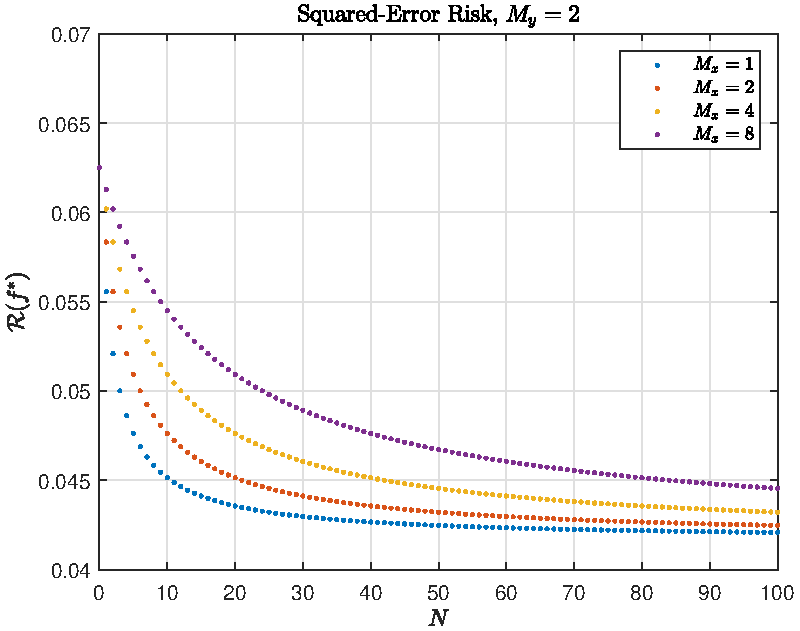
\includegraphics[scale=1.0]{Risk_SE_IO_N.pdf}
\caption{Optimal Squared-Error Risk vs training set size for various input set sizes}
\label{fig:Risk_SE_IO_N}
\end{figure}

\begin{figure}
\centering
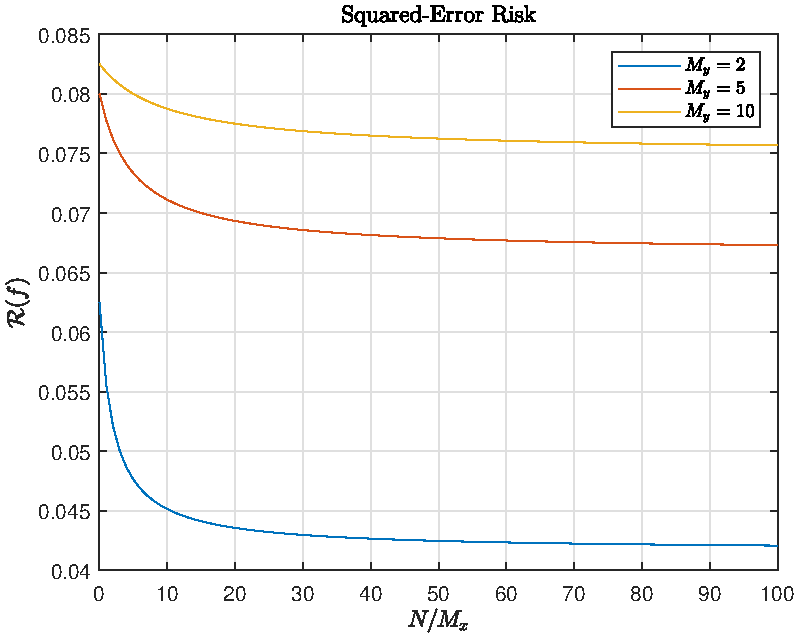
\includegraphics[scale=1.0]{Risk_SE_IO_N-Mx.pdf}
\caption{Optimal Squared-Error Risk vs $N/M_x$}
\label{fig:Risk_SE_IO_N-Mx}
\end{figure}
















\section{Applications: basic uniform}



\subsection{Classification: the 0-1 Loss} \label{sec:uniform_basic_apps_01}


\subsubsection{Optimal Learner: the MAP class estimate}

To determine the optimal learning function $f$, we combine the loss function \eqref{loss_01} with the posterior PMF of equation \eqref{P_y_D_basic}; the conditional expected loss reduces to
\begin{IEEEeqnarray}{rCl}
\text{E}_{\yrm | \Drm} \big[ \mathcal{L}(h,\yrm) \big] & = & 1 - \text{P}_{\yrm | \Drm}(h | \Drm) \\
& = & 1 - \left( \frac{M}{N+M} \right) M^{-1} - \left( \frac{N}{N+M} \right) \frac{\bar{N}(h;\Drm)}{N} \nonumber \;.  
\end{IEEEeqnarray}
Substituting into equation \eqref{f_opt_D}, the optimal learning function can be expressed as
\begin{IEEEeqnarray}{rCl}
f^*(\Drm) & = & \argmin_{h \in \Ycal} \text{E}_{\yrm | \Drm}\left[ 1 - \text{P}_{\yrm | \Drm}(h | \Drm)  \right] \\
& = & \argmax_{h \in \Ycal} \text{P}_{\yrm | \Drm}(h | \Drm) \nonumber \\
& = & \argmax_{h \in \Ycal} \bar{N}(h;D) \nonumber \;.
\end{IEEEeqnarray}

Given our lack of prior confidence in any of the data-generating PMF's $\bm{\theta}$, the best class estimate is simply found by choosing the class most represented in the training set $\Drm$.


\subsubsection{Minimum Risk: the Probability of Error}
Now, we determine the minimum risk (probability of error for the 0-1 loss). Starting from equation \eqref{risk_min}, we formulate the risk as
\begin{IEEEeqnarray}{rCl} \label{risk_01_opt}
\mathcal{R}(f^*) & = & \text{E}_{\Drm} \Big[ \text{E}_{\yrm | \Drm} \big[ \mathcal{L}(f^*(\Drm),\yrm) \big] \Big]
= 1 - \text{E}_{\Drm} \left[ \max_{y} \text{P}_{\yrm | \Drm}(y | \Drm) \right] \\
& = & 1 - \text{E}_{\Drm} \left[ \frac{\max_{y \in \Ycal} \bar{N}(y;\Drm) + 1}{N+M} \right] \nonumber \\
& = & 1 - \left( \frac{M}{N+M} \right) M^{-1} - \left( \frac{N}{N+M} \right) \frac{\text{E}_{\Drm} \left[ \max_{y \in \Ycal} \bar{N}(y;\Drm) \right]}{N} \nonumber \;. 
\end{IEEEeqnarray}

Before refining this expression, observe how the minimum risk trends as $M$ increases for fixed training set size $N$. Clearly, $\lim_{M \to \infty} \mathcal{R}(f^*) = 1 - M^{-1}$. This should be intuitively satisfying -- the posterior PMF trends toward a discrete uniform distribution, the same as if no data had been observed at all (e.g. $\text{P}(\yrm) = M^{-1}$).

Next, we continue to find a closed-form expression for the optimal risk; to do so, we must evaluate the expectation over all possible training sets $\Drm$. It can be clearly shown that the expectation can instead be performed over random variable $\nbarrm = \bar{\bm{N}}(\Drm)$, that is,
\begin{equation}
\text{E}_{\Drm} \left[ \max_y \bar{N}(y;\Drm) \right] = \text{E}_{\nbarrm} \left[ \max_y \bar{\nrm}(y) \right] \;.
\end{equation}

In Appendix \ref{app:E_N_max}, we determine the cumulative mass function (CMF) of $\bar{\nrm}_{\text{max}} = \max_y \bar{\nrm}(y)$, 
\begin{IEEEeqnarray}{rCl}
F_{\bar{\nrm}_{\text{max}}}(n) & = & \text{P}\left( \bar{\nrm}_{\text{max}} \leq n \right) \\
& = & \binom{N+M-1}{M-1}^{-1} \sum_{m=1}^M \binom{M}{m} (-1)^{M-m} \nonumber \\
&& \quad \binom{m(n+1)-N-1}{M-1} U\left( n+1-\left\lceil\frac{N+M}{m}\right\rceil \right) \nonumber \;,
\end{IEEEeqnarray}
where $U: \mathbb{R} \mapsto \{0,1\}$ is the continuous step function. Clearly, the PMF is zero outside of the interval $[0,N+M]$; the expected value is thus
\begin{IEEEeqnarray}{rCl}
\text{E}_{\bar{\bm{n}}} \left[ \bar{\nrm}_{\text{max}} \right] & = & \sum_{n=0}^{N+M} n \big( F_{\bar{\nrm}_{\text{max}}}(n) - F_{\bar{\nrm}_{\text{max}}}(n-1) \big) \\
& = & N + M - \sum_{n=0}^{N+M-1} F_{\bar{\nrm}_{\text{max}}}(n) \nonumber \\
& = & N + M - \binom{N+M-1}{M-1}^{-1} \sum_{m=1}^M \binom{M}{m} (-1)^{M-m} \nonumber \\
&& \quad \sum_{n = \left\lceil \frac{N+M}{m} \right\rceil}^{N+M} \binom{mn-N-1}{M-1} \nonumber \;.
\end{IEEEeqnarray}

This general equation has not been reduced to a more tractable form. Using it it conjunction with equation \eqref{risk_01_opt}, we have the expression for the optimal risk,
\begin{IEEEeqnarray}{rCl}
\mathcal{R}(f^*) & = & 1 - \text{E}_{\Drm} \left[ \frac{\max_y \bar{N}(y;\Drm) + 1}{N+M} \right] \\
& = & \frac{1}{N+M} \left[ -1 + \binom{N+M-1}{M-1}^{-1} \sum_{m=1}^M \binom{M}{m} (-1)^{M-m} \sum_{n = \left\lceil \frac{N+M}{m} \right\rceil}^{N+M} \binom{mn-N-1}{M-1}  \right] \nonumber \\
& = & \frac{-1}{N+M} \left[ 1 + \sum_{m=1}^M \binom{M}{m} (-1)^m \sum_{n = \left\lceil \frac{N+M}{m} \right\rceil}^{N+M} \prod_{l=1}^{M-1} \left( 1 - \frac{mn}{N+l} \right) \right] \nonumber \;.
%& = & \frac{M - 1 +\binom{N+M-1}{M-1}^{-1} \sum_{m=1}^M \binom{M}{m} (-1)^{M-m} \sum_{n = \left\lceil \frac{N+M}{m} \right\rceil}^N \binom{mn-N-1}{M-1}}{N+M} \;.
\end{IEEEeqnarray}
Figure \ref{fig:Risk_01_vsN} displays the risk as a function of $N$ for select values of $M$. Observe that even for binary classification, the optimal risk asymptotes quickly.

PGR: Havent found closed form for summation over n. Can a bound be found instead???

\begin{figure}
\centering
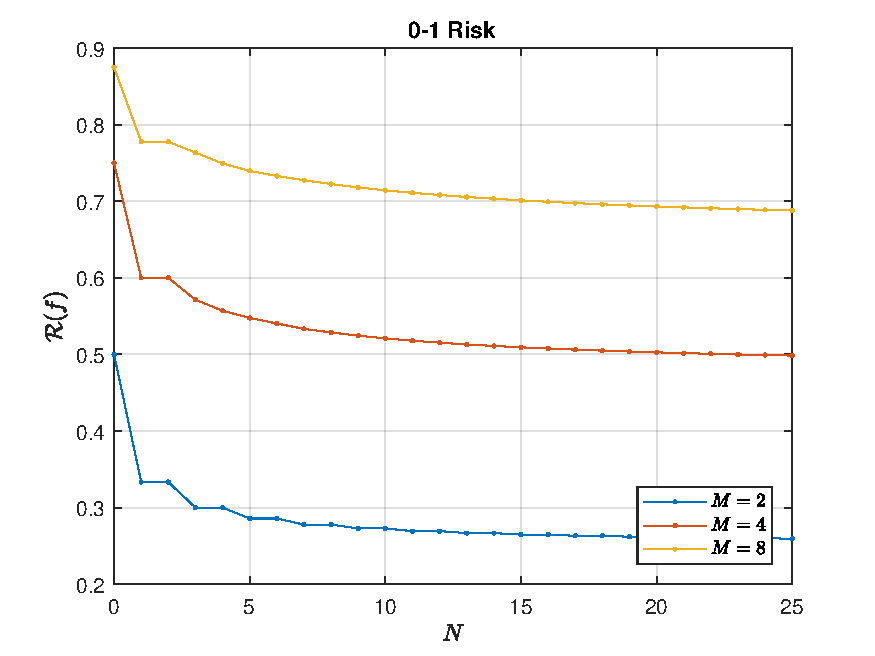
\includegraphics[scale=1.0]{Risk_01_vsN.pdf}
\caption{Optimal 0-1 Risk, vs. Training Set volume $N$}
\label{fig:Risk_01_vsN}
\end{figure}

The performance of this optimal decision function in the limit of training set volume $N \to \infty$ is of interest. Fortunately, the expectation $\text{E}_{\bar{\bm{\mathrm{n}}}} \big[ \max_y \bar{\nrm}(y) \big]$ can be represented more compactly in this limit. As detailed in Appendix \ref{app:E_N_max},
\begin{equation}
\lim_{N \to \infty} \frac{\text{E}_{\bar{\bm{\mathrm{n}}}} \big[ \max_y \bar{\nrm}(y) \big]}{N} = \frac{1}{M} \sum_{m=1}^M \frac{1}{m} \;.
\end{equation}

Note that this summation has no closed-form -- it is a Harmonic number. Note also that if the class set is countably infinite, this summation can be represented as
\begin{IEEEeqnarray}{rCl}
\lim_{M \to \infty} \frac{1}{M} \sum_{m=1}^M \frac{1}{m} & = & \lim_{M \to \infty} \frac{\text{ln}(M)}{M} \\
& = & \lim_{M \to \infty} \frac{1}{M} = 0 \nonumber \;.
\end{IEEEeqnarray}

PGR: harmonic reference???

Substituting the limiting form of the expectation into equation \eqref{risk_01_opt}, we determine the optimal risk
\begin{equation}
\lim_{N \to \infty} \mathcal{R}(f^*)  = \lim_{N \to \infty} \left( 1 - \frac{\text{E}_{\Drm} \left[ \max_y \bar{N}(y;\Drm) \right]}{N} \right) = 1 - \frac{1}{M} \sum_{m=1}^M \frac{1}{m} \;,
\end{equation}
which provides a lower bound to the risk that any learner can achieve with any volume of training data. Figure \ref{fig:Risk_01_LB} displays this risk, as well as the optimal risk when no training data is available. Note the margin in the probability of error between the optimal $N=0$ and $N \to \infty$ learners. For binary classification (the simplest case), we see a modest reduction from 0.5 to 0.25 error; for higher values of $M$, the probability of error increases towards unity. Clearly, this level of error is unacceptable for most applications. Nonetheless, it is the minimum risk for the problem we have formulated -- this results from our choosing a non-informative prior over $\bm{\Theta}$.

\begin{figure}
\centering
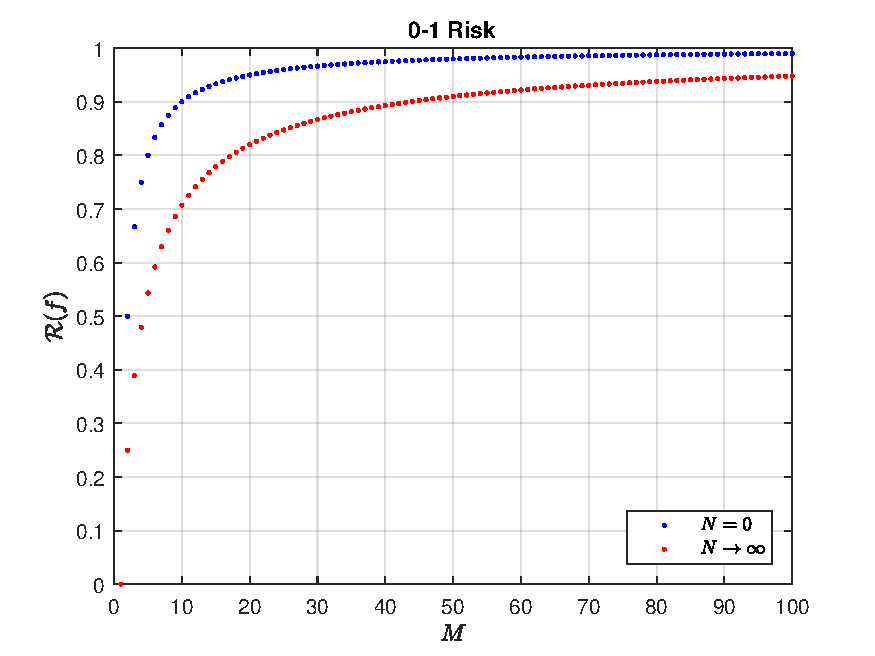
\includegraphics[scale=1.0]{Risk_01_LB.pdf}
\caption{Optimal 0-1 Risk, Upper and Lower bounds}
\label{fig:Risk_01_LB}
\end{figure}

PGR: PLOT RISK VS THETA???



\subsection{Regession: the Squared-Error Loss}

The squared-error (SE) loss function is by far the most commonly used loss function for regression, or in fact any estimation problems where the variable of interest is continuous. This is due to its convexity, which allows easy determination of the minimizing learner. 

Up until now, the $M$ elements of the output set $\Ycal$ have remained abstract, without imposing any order to the elements (besides the indexing notation). For regression, we will assign numerical values to the unobserved output; specifically, $\Ycal = \{1,\ldots,M\}$. Additionally, we will allow the learning function's decision to lie on the real line; thus, $\Hcal = \mathbb{R} \supset \Ycal$.

The loss function is defined as,

\begin{equation}
\mathcal{L}(h,y) = (h-y)^2 \;.
\end{equation}


\subsubsection{Optimal Learner: The Posterior Mean}

To determine the optimal learning function, we expand the conditional expectation
\begin{IEEEeqnarray}{rCl} \label{f_opt_mse}
\text{E}_{\yrm | \Drm} \big[ \mathcal{L}(h,\yrm) \big] & = & \sum_{y=1}^M (h-y)^2 \text{P}_{\yrm | \Drm}(y | \Drm) \;.
\end{IEEEeqnarray}
Clearly, this function is quadratic and thus convex over $\Hcal$ -- the minimizing value is the sole stationary point. Differentiating and equating to zero, we find
\begin{IEEEeqnarray}{rCl}
f^*(\Drm) & = & \argmin_{h \in \mathbb{R}} \text{E}_{\yrm | \Drm} \left[ (h-\yrm)^2 \right] \\
& = & \sum_{y=1}^M y \text{P}_{\yrm | \Drm}(y | \Drm) \equiv \mu_{\yrm | \Drm} \nonumber \\
& = & \left(\frac{M}{N+M}\right) \frac{M+1}{2} + \left(\frac{N}{N+M}\right) \sum_{y=1}^M y \frac{\bar{N}(y;\Drm)}{N} \nonumber \\
& = & \left(\frac{M}{N+M}\right) \frac{M+1}{2} + \left(\frac{N}{N+M}\right) \frac{1}{N} \sum_{n=1}^N \Drm(n) \nonumber \;,
\end{IEEEeqnarray}
where we have substituted in equation \eqref{P_y_D} for the posterior PMF. 

The interpretation of the posterior as a mixture distribution is notable here; the optimal learner is a convex combination of two PMF mean values. Furthermore, the second mean can be represented as the average value in the training set $\Drm$.

The mixture of moments prompts analysis of the optimal learner's asymptotic behavior. Clearly, if the unobserved variable $\yrm$ is drawn from an infinite set (e.g. $\mathbb{N}$), such that $M \to \infty$, then the minimum squared error (MSE) estimate is the average value of the set $\Ycal$ and does not depend on the training data at all. Conversely, if $M$ is finite, then as the training data volume increases, the optimal learner trends toward the average value of the observed set $\Drm$.  



\subsubsection{Minimum Risk: The Expected Posterior Variance}

In this section, we will analyze the minimum expected squared-error achieved by the optimal learner in equation \eqref{f_opt_mse}. Substituting into equation \eqref{risk_min}, we have
\begin{IEEEeqnarray}{rCl}
\mathcal{R}(f^*) & = & \text{E}_{\Drm} \Big[ \text{E}_{\yrm | \Drm} \big[ \mathcal{L}(f^*(\Drm),\yrm) \big] \Big]
= \text{E}_{\Drm} \Big[ \text{E}_{\yrm | \Drm} \big[ (\yrm - \mu_{\yrm | \Drm})^2 \big] \Big] \\
& = &  \text{E}_{\Drm} \left[ \Sigma_{\yrm | \Drm} \right] \nonumber \\
& = & \text{E}_{\nbarrm} \left[ \Sigma_{\yrm | \nbarrm} \right] \nonumber \;,
\end{IEEEeqnarray}
where we use $\Sigma_{\yrm | \nbarrm}$ to simplify the notation for the variance of the posterior PMF.

PGR: REWORK TO MIRROR I/O SECTION METHOD ???!!!

First, we formulate the conditional variance,
\begin{IEEEeqnarray}{rCl}
\Sigma_{\yrm | \nbarrm} & = & \text{E}_{\yrm | \nbarrm}\big[ \yrm^2 \big]
- \big( \text{E}_{\yrm | \nbarrm}[\yrm] \big)^2 \\
& = & \sum_{y=1}^M y^2 \text{P}_{\yrm | \nbarrm}(y | \nbarrm) - \left( \sum_{y=1}^M y \text{P}_{\yrm | \nbarrm}(y | \nbarrm) \right)^2 \nonumber \\
& = & \sum_{y=1}^M y^2 \frac{\bar{\nrm}(y) + 1}{N+M} - \sum_{y=1}^M y \sum_{y'=1}^M y' \frac{\big( \bar{\nrm}(y) + 1 \big) \big( \bar{\nrm}(y') + 1 \big)}{(N+M)^2} \nonumber \;.
\end{IEEEeqnarray}



%First, we formulate the conditonal variance. To simplify the presentation, we express the mixture distribution as,
%
%\begin{equation}
%\text{P}_{\yrm | \nbarrm}(m) = \left(\frac{M}{N+M}\right) \text{P}^\text{prior}_{\yrm}(m) + \left(\frac{N}{N+M}\right) \text{P}^\text{prior}_{\yrm | \nbarrm}(m) \;,
%\end{equation}
%
%and the mean and variance of each distribution,
%
%\begin{IEEEeqnarray}{C}
%\mu^\text{prior}_{\yrm} = \frac{M+1}{2} \;, \\
%\Sigma^\text{prior}_{\yrm} = \frac{(M+1)(M-1)}{12} \;, \\
%\mu^\text{data}_{\yrm | \nbarrm} = \frac{1}{N} \sum_{m=1}^M m \bar{\nrm}_m \;, \\
%\Sigma^\text{data}_{\yrm | \nbarrm} = \frac{1}{N}\sum_{m=1}^M m^2 \bar{\nrm}_m 
%- \frac{1}{N^2} \left( \sum_{k=1}^M k \bar{\nrm}_k \right)^2 \;.
%\end{IEEEeqnarray}
%
%As demonstrated in REFERENCE???, the conditional variance equates to,
%
%\begin{IEEEeqnarray}{rCl}
%\Sigma_{\yrm | \nbarrm} & = & 
%\sum_{m=1}^M \text{P}_{\yrm | \nbarrm}(m) \left( m - \mu_{\yrm | \nbarrm} \right)^2 \\
%& = & \left(\frac{M}{N+M}\right) \Sigma^\text{prior}_{\yrm} 
%+ \left(\frac{N}{N+M}\right) \Sigma^\text{data}_{\yrm | \nbarrm} \\
%&& \quad + \left(\frac{M}{N+M}\right)\left(\frac{N}{N+M}\right) \left( \mu^\text{prior}_{\yrm} - \mu^\text{data}_{\yrm | \nbarrm} \right)^2 \;.
%\end{IEEEeqnarray}

Inspection of the above form shows that the variance is quadratic in $\nbarrm$ -- as such, the expected conditional variance will depend on $\text{P}(\nbarrm)$ only via the first and second joint moments of the distribution. In Appendix \ref{app:E_N_bar}, these moments are determined to be
\begin{equation}
\text{E}[\nbarrm] = \frac{N}{M} \bm{1}_{M \times 1}
\end{equation}
and
\begin{equation}
\text{E}\big[ \nbarrm \nbarrm^\text{T} \big] = \frac{N \left( (N+M)\textbf{I} + (N-1)\bm{1}\bm{1}^\text{T} \right)}{M(M+1)} \;.
\end{equation}

After substitution into the above form for the conditional variance APPENDIX???, we solve for the minimum risk,
\begin{IEEEeqnarray}{rCl} \label{Risk_SE_opt}
\mathcal{R}(f^*) & = & \text{E}_{\nbarrm} \left[ \Sigma_{\yrm | \nbarrm} \right] \\
& = & \frac{M(M-1)(N+M+1)}{12(N+M)} \nonumber \\
& = & \left(\frac{M}{N+M}\right) \frac{(M+1)(M-1)}{12} + \left(\frac{N}{N+M}\right) \frac{M(M-1)}{12} \nonumber \;. 
\end{IEEEeqnarray}

Note that without training data ($N=0$), the risk is simply equal to $\Sigma_{\yrm}$. Conversely, as $N \to \infty$, we have $\mathcal{R}(f^*) = \frac{M(M-1)}{12}$, which constitutes a reduction in risk by a factor of $\frac{M}{M+1}$; also, note that this asymptotic loss is the same that would be acheived by a clairvoyant learning function (i.e. $\bm{\theta}$ is observable and superscedes the training data $\Drm$ for design).

To enable better visualization of the dependency of optimal risk on $N$ and $M$, we restrict the unobserved variable to the unit interval by scaling the output as $\yrm \gets \yrm/M$. As a result, the conditional variance and thus the optimal risk in equation \eqref{Risk_SE_opt} is scaled by $M^{-2}$. Figure \ref{fig:Risk_SE_LB} display the upper ($N=0$) and lower ($N \to \infty$) bounds for the minimum risk. Additonally, Figure \ref{fig:Risk_SE_vsN} shows how the minimum risk decreases with $N$ for various values of $M$.


\begin{figure}
\centering
\includegraphics[scale=1.0]{Risk_SE_LB.pdf}
\caption{Optimal Squared-Error Risk, Upper and Lower bounds}
\label{fig:Risk_SE_LB}
\end{figure}

\begin{figure}
\centering
\includegraphics[scale=1.0]{Risk_SE_vsN.pdf}
\caption{Optimal Squared-Error Risk, vs. Training Set volume $N$}
\label{fig:Risk_SE_vsN}
\end{figure}






\section{Applications: Dir basic}



\subsection{Classification: the 0-1 Loss}

In this section we generalize the previous results for the 0-1 loss function $\mathcal{L}(h,y) = 1 - \delta[h,y]$ and the class hypothesis space $\Hcal = \Ycal$.

PGR: CHECK BELOW... General, suboptimal forms for risk? See early notes for SE; for 01,

\begin{IEEEeqnarray}{rCl}
\mathcal{R}(f) & = & 1 - \text{E}_{\bm{\theta}} \bigg[ \text{E}_{\Drm | \bm{\theta}} \Big[ \text{E}_{y | \bm{\theta}} \big[ \delta[f(\Drm),y] \big] \Big] \bigg] \\
& = & 1 - \text{E}_{\bm{\theta}} \bigg[ \text{E}_{\Drm | \bm{\theta}} \Big[ \theta\big( f(\Drm) \big) \Big] \bigg] \nonumber \\
& = & 1 - \frac{\text{E}_{\nbarrm} \Big[ \alpha\big( f(\bar{\nrm}) \big) + \bar{\nrm}\big( f(\bar{\nrm}) \big) \Big]}{\alpha_0 + N} \nonumber
\end{IEEEeqnarray}



\subsubsection{Optimal Learner}

The optimal classifier again chooses the value $\yrm$ that has the maximum value in the conditional PMF, such that
\begin{IEEEeqnarray}{rCl}
f^*(\Drm) & = & \argmax_{y \in \Ycal} \text{P}_{\yrm | \Drm}(y | \Drm) \\
& = & \argmax_{y \in \Ycal} \left( \alpha(y) + \bar{N}(y;\Drm) \right) \nonumber \;.
\end{IEEEeqnarray}

With the subjective prior, the minimum risk hypothesis is no longer just a majority decision rule; the frequency of occurrence of each value $\yrm$ must be combined with the relative values of the parameter function $\alpha$. 



\subsubsection{Minimum Risk}

The minimum probability of error is
\begin{IEEEeqnarray}{rCl}
\mathcal{R}(f^*) & = & 1 - \frac{\text{E}_{\nbarrm} \Big[ \max_{y \in \Ycal} \big( \alpha(y) + \bar{\nrm}(y) \big) \Big]}{\alpha_0 + N}
\end{IEEEeqnarray}


PGR: no closed-forms found???

PGR: comment on simulation!

For $N = 0$, we have $\mathcal{R}(f^*) = 1 - \max_{y \in \Ycal} \alpha(y) / \alpha_0$. 

For $N \to \infty$, we have $\mathcal{R}(f^*) = ???$.

For $\alpha_0 \to 0$ and $N > 1$, we have $\mathcal{R}(f^*) = 0$.

For $\alpha_0 \to \infty$, we have $\mathcal{R}(f^*) = 1 - \max_{y \in \Ycal} \alpha(y) / \alpha_0$.



\begin{figure}
\centering
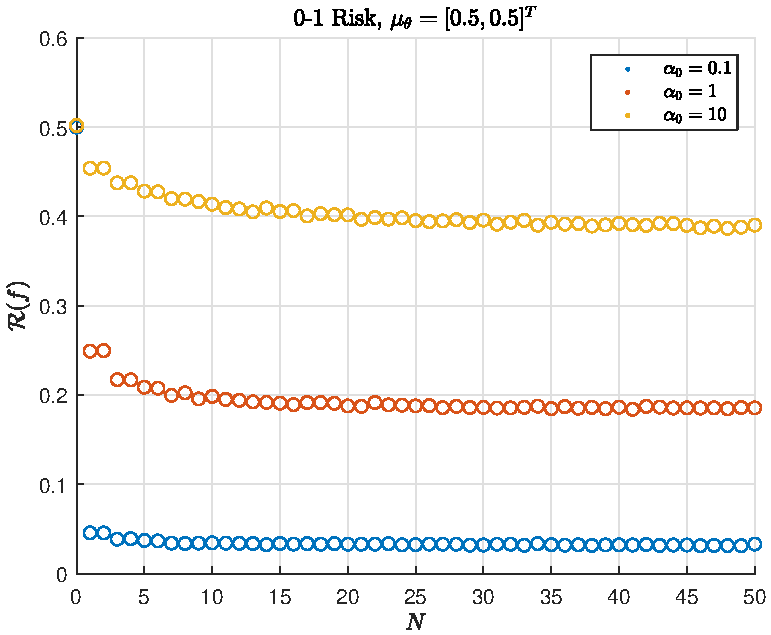
\includegraphics[scale=1.0]{Risk_01_Dir_N.pdf}
\caption{Optimal 0-1 Risk vs $N$}
\label{fig:Risk_01_Dir_N}
\end{figure}

\begin{figure}
\centering
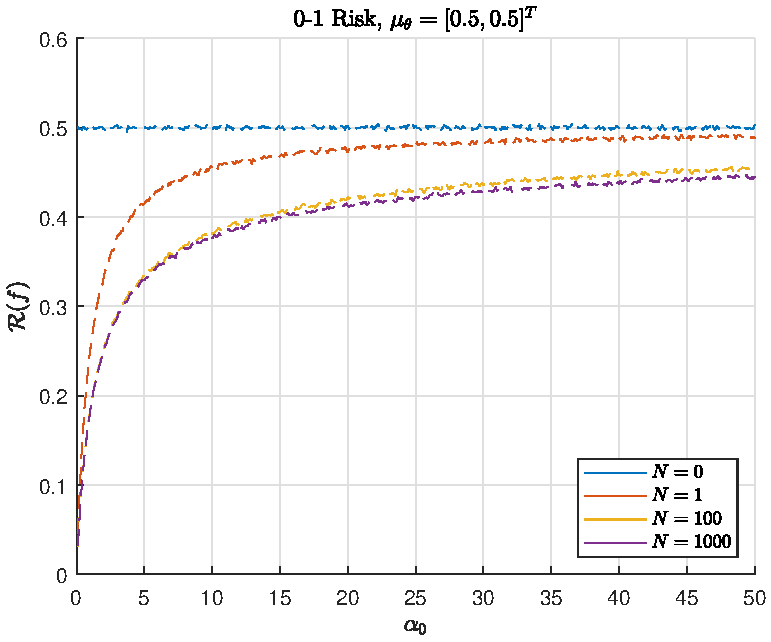
\includegraphics[scale=1.0]{Risk_01_Dir_alpha0.pdf}
\caption{Optimal 0-1 Risk vs $\alpha_0$}
\label{fig:Risk_01_Dir_alpha0}
\end{figure}

\begin{figure}
\centering
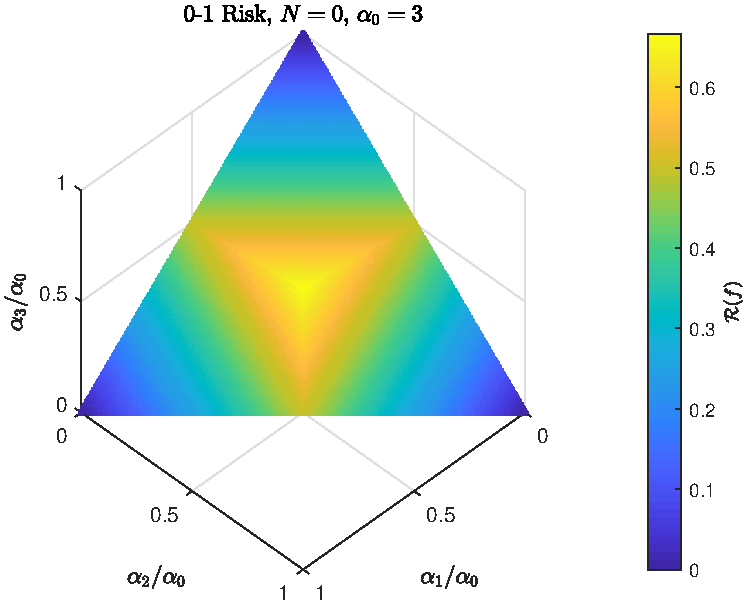
\includegraphics[scale=1.0]{Risk_01_Dir_muTheta_N_0_a0_3.pdf}
\caption{Optimal 0-1 Risk vs $\mu_{\bm{\theta}}$}
\label{fig:Risk_01_Dir_muTheta_N_0_a0_3}
\end{figure}

\begin{figure}
\centering
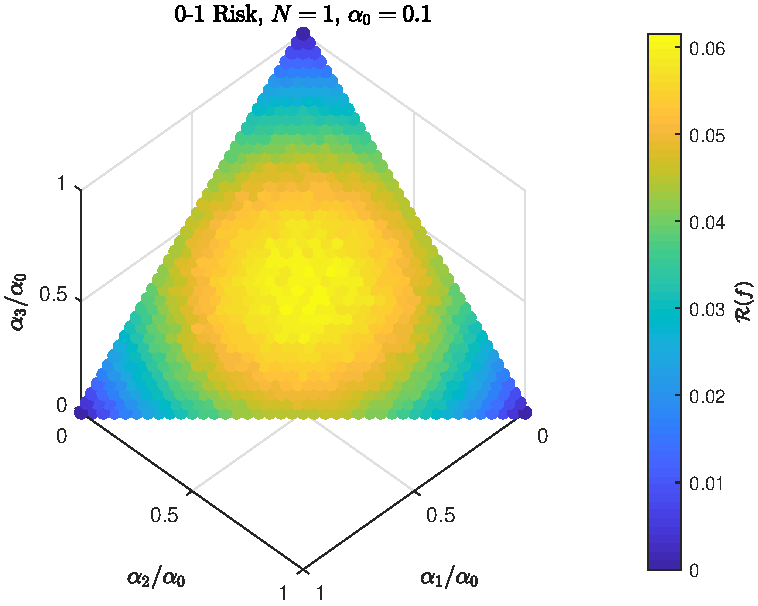
\includegraphics[scale=1.0]{Risk_01_Dir_muTheta_N_1_a0_01.pdf}
\caption{Optimal 0-1 Risk vs $\mu_{\bm{\theta}}$}
\label{fig:Risk_01_Dir_muTheta_N_1_a0_01}
\end{figure}

\begin{figure}
\centering
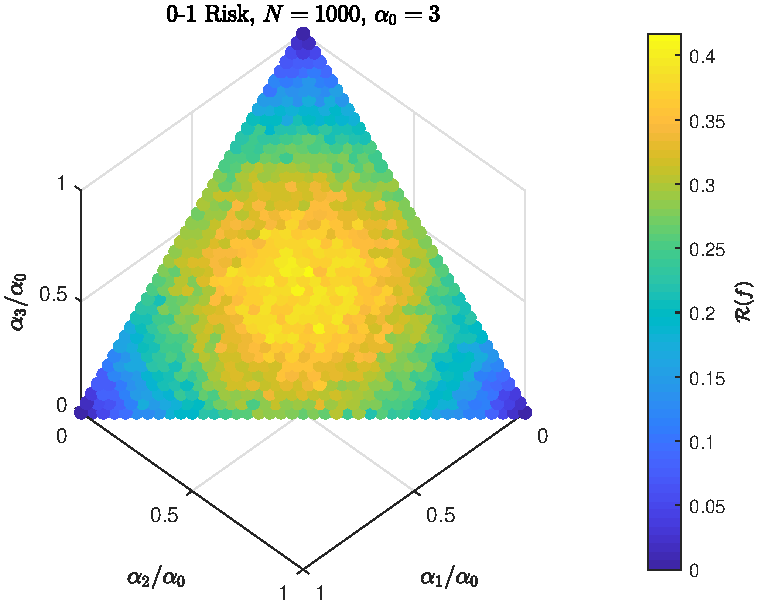
\includegraphics[scale=1.0]{Risk_01_Dir_muTheta_N_1000_a0_3.pdf}
\caption{Optimal 0-1 Risk vs $\mu_{\bm{\theta}}$}
\label{fig:Risk_01_Dir_muTheta_N_1000_a0_3}
\end{figure}





\subsection{Regression: the Squared-Error Loss}

PGR: Use finite hypothesis space instead, wait for continuous DP???

PGR: Provide suboptimal risk in terms of x,D only???


Here, we generalize the results for a regression application with a squared-error loss
\begin{equation}
\mathcal{L}(h,y) = (h-y)^2 \;.
\end{equation}

Again we choose for the regression function to map to $\Hcal = \mathbb{R}$, a superset of $\Ycal = \{1,\ldots,M\}$.

\begin{IEEEeqnarray}{rCl}
\mathcal{R}(f) & = & \text{E}_{\bm{\theta}} \Bigg[ \text{E}_{\Drm | \bm{\theta}} \bigg[ \text{E}_{\yrm | \bm{\theta}} \Big[ \big( f(\Drm)-\yrm \big)^2 \Big] \bigg] \Bigg] \\
& = & \text{E}_{\bm{\theta}} \Big[ \text{E}_{\yrm | \bm{\theta}} \big[ (\yrm - \mu_{\yrm | \bm{\theta}})^2 \big] \Big] + \text{E}_{\bm{\theta}} \bigg[ \text{E}_{\Drm | \bm{\theta}} \Big[ \big( f(\Drm) - \mu_{\yrm | \bm{\theta}} \big)^2 \Big] \bigg] \nonumber \\
& = & \text{E}_{\bm{\theta}} \left[ \Sigma_{\yrm | \bm{\theta}} \right] + \text{E}_{\bm{\theta}} \bigg[ \text{E}_{\Drm | \bm{\theta}} \Big[ \big( f(\Drm) - \mu_{\yrm | \bm{\theta}} \big)^2 \Big] \bigg] \nonumber
\end{IEEEeqnarray}


\subsubsection{Optimal Learner}

The optimal function is again the expected value of the output conditional PMF,
\begin{IEEEeqnarray}{rCl} \label{eq:f_opt_se_dir_basic}
f^*(\Drm) & = & \argmin_{h \in \mathbb{R}} \text{E}_{\yrm | \Drm} \big[ (h-\yrm)^2 \big]  \\
& = & \mu_{\yrm | \Drm} = \text{E}_{\bm{\theta} | \Drm} \left[ \mu_{\yrm | \bm{\theta}} \right] \nonumber \\
& = & \left( \frac{\alpha_0}{\alpha_0+N} \right) \sum_{y \in \Ycal} y \frac{\alpha(y)}{\alpha_0} +  \left( \frac{N}{\alpha_0+N} \right) \frac{1}{N} \sum_{n=1}^N \Drm(n) \nonumber \;.
\end{IEEEeqnarray}
Now the data-independent term in the convex combination is the expected value of the PMF $\text{P}(\yrm) = \text{E}_{\bm{\theta}}\big[ \theta(\yrm) \big]$.


\subsubsection{Minimum Risk}

PGR: let output set remain abstract instead of counting numbers??? Ch1.

The minimum expected squared-error realized when using the conditional mean in equation \eqref{eq:f_opt_se_dir_basic} is once again the expected conditional variance
\begin{IEEEeqnarray}{rCl}
\mathcal{R}(f^*) & = & \text{E}_{\Drm} \left[ \Sigma_{\yrm | \Drm} \right]
= \text{E}_\mathrm{\nbarrm} \left[ \Sigma_{\yrm | \mathrm{\nbarrm}} \right] \\
& = & \text{E}_{\bm{\theta}} \left[ \Sigma_{\yrm | \bm{\theta}} \right] + \text{E}_{\Drm} \bigg[ \text{E}_{\bm{\theta} | \Drm} \Big[ \big( \mu_{\yrm | \bm{\theta}} - \text{E}_{\bm{\theta} | \Drm}[\mu_{\yrm | \bm{\theta}}] \big)^2 \Big] \bigg] \nonumber \\
& = & \text{E}_{\bm{\theta}} \left[ \Sigma_{\yrm | \bm{\theta}} \right] + \text{E}_{\Drm} \Big[ \text{C}_{\bm{\theta} | \Drm} \left[ \mu_{\yrm | \bm{\theta}} \right] \Big] \nonumber \;,
\end{IEEEeqnarray}
where we choose to perform the expectation over $\nbarrm$; this is feasible since the marginal and conditional distributions of $\Drm$ used here are dependent only through the transform $\bar{N}$. Above, we introduce the $\text{C}$ operator, which provides the variance of a function of a random variable, 
\begin{equation}
\text{C}_{\xrm}\big[g(\xrm)\big] = \text{E}_{\xrm} \bigg[ \Big( g(\xrm) - \text{E}_{\xrm}\big[g(\xrm)\big] \Big)^2 \bigg] \;.
\end{equation}

The conditional varance is now
\begin{IEEEeqnarray}{rCl}
\Sigma_{\yrm | \nbarrm} & = & \text{E}_{\yrm | \nbarrm}[\yrm^2]
- \big( \text{E}_{\yrm | \nbarrm}[\yrm] \big)^2 \\
& = & \sum_{y \in \Ycal} y^2 \frac{\alpha(y) + \bar{\nrm}(y)}{\alpha_0 + N} - \sum_{y' \in \Ycal} y' \sum_{y'' \in \Ycal} y'' \frac{\big( \alpha(y') + \bar{\nrm}(y') \big) \big(\alpha(y'') + \bar{\nrm}(y'') \big)}{(\alpha_0 + N)^2} \nonumber \;.
\end{IEEEeqnarray}

Using the first and second moments of the Dirichlet-Multinomial PMF, we take the expectation over $\nbarrm$ and find the minimum risk,
\begin{IEEEeqnarray}{rCl}
\mathcal{R}(f^*) & = & \frac{\alpha_0 (\alpha_0+N+1)}{(\alpha_0+1)(\alpha_0+N)} 
\left[ \left( \sum_{y \in \Ycal} \frac{\alpha(y)}{\alpha_0} y^2 \right) - \left( \sum_{y \in \Ycal} \frac{\alpha(y)}{\alpha_0} y \right)^2 \right] \\
& = & \frac{\alpha_0 (\alpha_0+N+1)}{(\alpha_0+1)(\alpha_0+N)} 
\left[ \left( \sum_{y \in \Ycal} \text{P}_{\yrm}(y) y^2 \right) - \left( \sum_{y \in \Ycal} \text{P}_{\yrm}(y) y \right)^2 \right] \nonumber \\
& = & \frac{1+(\alpha_0+N)^{-1}}{1+(\alpha_0)^{-1}} \Sigma_{\yrm} \nonumber \;.
\end{IEEEeqnarray}

Observe that the minimum squared-error is the marginal variance $\Sigma_{\yrm}$ scaled by a factor dependent on the the number of training samples $N$ and the model prior concentration paramter $\alpha_0$. Figures \ref{fig:Risk_SE_Dir_N} and \ref{fig:Risk_SE_Dir_alpha0} provide visualizations of how these parameters affect the optimal risk for a given model mean $\mu_{\bm{\theta}} = \bm{\alpha}/\alpha_0$. Without training data, $\mathcal{R}(f^*) = \Sigma_{\yrm}$; as $N \to \infty$, the risk is reduced by $\alpha_0 / (\alpha_0+1)$. Additionally, note how the risk changes for different model prior concentrations: as the prior PDF becomes more concentrated, the scaling factor trends toward unity and the risk increases; as $\alpha_0 \to 0$, the minimum risk trends toward zero (given $N > 0$). 

It may not seem intutitve for performance to improve when the prior knowledge is less definitive; this is a result of the Dirichlet PDF weight shifting towards the Euclidean basis vectors as the concentration parameter decreases. Although these PMF's are maximally different (uncorrelated), they all lead to zero minimum risk; this is implied by Figure \ref{fig:Risk_SE_Dir_muTheta}. The optimal learner will simply use the empirical distribution supplied via the training data - this allows identification of $\bm{\theta}$ even with a single training pair and leads to predictions that match the single class represented in $D$.




\begin{figure}
\centering
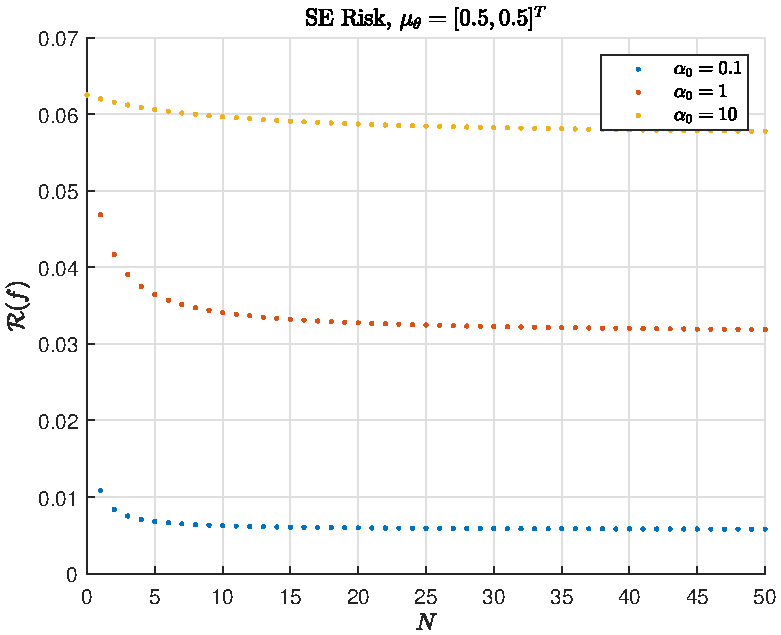
\includegraphics[scale=1.0]{Risk_SE_Dir_N.pdf}
\caption{Optimal Squared-Error Risk vs $N$}
\label{fig:Risk_SE_Dir_N}
\end{figure}

\begin{figure}
\centering
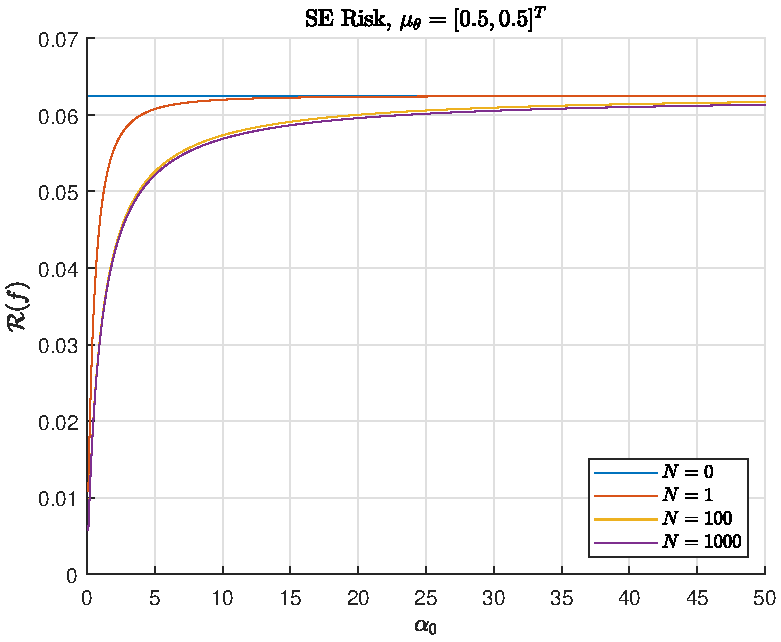
\includegraphics[scale=1.0]{Risk_SE_Dir_alpha0.pdf}
\caption{Optimal Squared-Error Risk vs $\alpha_0$}
\label{fig:Risk_SE_Dir_alpha0}
\end{figure}

\begin{figure}
\centering
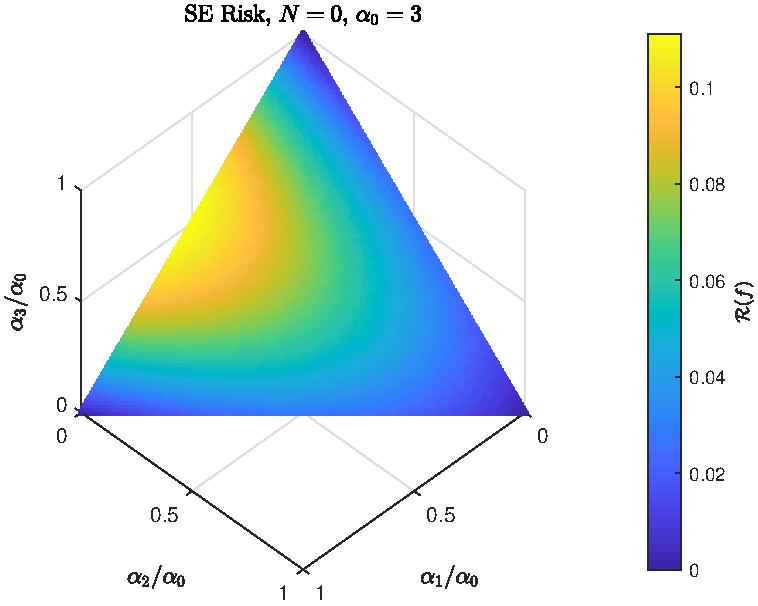
\includegraphics[scale=1.0]{Risk_SE_Dir_muTheta.pdf}
\caption{Optimal Squared-Error Risk vs $\mu_{\bm{\theta}}$}
\label{fig:Risk_SE_Dir_muTheta}
\end{figure}

PGR: scatter plots: use yi indexing, P instead of alpha???













\section{Applications: Dir general}



\subsection{Regression: the Squared-Error Loss}

\begin{IEEEeqnarray}{rCl}
\mathcal{R}(f) & = & \text{E}_{\bm{\theta}} \Bigg[ \text{E}_{\Drm | \bm{\theta}} \bigg[ \text{E}_{\yrm,\xrm | \bm{\theta}} \Big[ \big( f(\xrm,\Drm)-\yrm \big)^2 \Big] \bigg] \Bigg] \\
& = & \text{E}_{\xrm,\bm{\theta}} \Big[ \text{E}_{\yrm | \xrm,\bm{\theta}} \big[ (\yrm - \mu_{\yrm | \xrm,\bm{\theta}})^2 \big] \Big] + \text{E}_{\bm{\theta}} \bigg[ \text{E}_{\xrm,\Drm | \bm{\theta}} \Big[ \big( f(\xrm,\Drm) - \mu_{\yrm | \xrm,\bm{\theta}} \big)^2 \Big] \bigg] \nonumber \\
& = & \text{E}_{\xrm,\bm{\theta}} \left[ \Sigma_{\yrm | \xrm,\bm{\theta}} \right] + \text{E}_{\bm{\theta}} \bigg[ \text{E}_{\xrm,\Drm | \bm{\theta}} \Big[ \big( f(\xrm,\Drm) - \mu_{\yrm | \xrm,\bm{\theta}} \big)^2 \Big] \bigg] \nonumber
\end{IEEEeqnarray}



\subsubsection{Optimal Learner}

The optimal classifier is the expected value of $\yrm$ given the training data and the observed value of $\xrm$, such that
\begin{IEEEeqnarray}{rCl}
f^*(\xrm,\Drm) & = & \mu_{\yrm | \xrm,\Drm}  = \text{E}_{\bm{\theta} | \xrm,\Drm} \left[ \mu_{\yrm | \xrm,\bm{\theta}} \right] \\
& = & \left( \frac{\alpha'(\xrm)}{\alpha'(\xrm) + N'(\xrm;\Drm)} \right) \sum_{y \in \Ycal} y \frac{\alpha(y,\xrm)}{\alpha'(\xrm)} \nonumber \\
&& \quad + \left( \frac{N'(\xrm;\Drm)}{\alpha'(\xrm) + N'(\xrm;\Drm)} \right) \frac{\sum_{n=1}^N \delta\big[ \xrm,\Xrm(n) \big] \Yrm(n)}{N'(\xrm;\Drm)} \nonumber \;.
\end{IEEEeqnarray}

Here, the data-dependent term in the convex combination is the average value of the training values $\Yrm(n)$ which have an input value $\Xrm(n)$ matching the novel observed value $\xrm$.



\subsubsection{Minimum Risk}

Generalizing from the basic model discussion, we again have
\begin{IEEEeqnarray}{rCl}
\mathcal{R}(f^*) & = & \text{E}_{\xrm,\Drm} \left[ \Sigma_{\yrm | \xrm,\Drm} \right]
= \text{E}_{\xrm,\mathrm{\nbarrm}} \left[ \Sigma_{\yrm | \xrm,\mathrm{\nbarrm}} \right] \\
& = & \text{E}_{\xrm,\bm{\theta}} \left[ \Sigma_{\yrm | \xrm,\bm{\theta}} \right] + \text{E}_{\xrm,\Drm} \left[ \text{C}_{\bm{\theta} | \xrm,\Drm} \left[ \mu_{\yrm | \xrm,\bm{\theta}} \right] \right] \nonumber \;,
\end{IEEEeqnarray}
where we choose to perform the expectation over $\nbarrm$. 

The conditional varance is now
\begin{IEEEeqnarray}{rCl}
\Sigma_{\yrm | \xrm,\nbarrm} & = & \text{E}_{\yrm | \xrm,\nbarrm}[\yrm^2] - \big( \text{E}_{\yrm | \xrm,\nbarrm}[\yrm] \big)^2 \;.
\end{IEEEeqnarray}

We will assess two expectations over the observables separately. First, we have,
\begin{IEEEeqnarray}{L}
\text{E}_{\xrm,\nbarrm} \left[ \text{E}_{\yrm | \xrm,\nbarrm}[\yrm^2] \right] \\
\quad = \text{E}_{\yrm}[\yrm^2] = \sum_{y \in \Ycal} y^2 \sum_{x \in \Xcal} \frac{\alpha(y,x)}{\alpha_0} \nonumber \\
\quad = \text{E}_{\xrm} \big[ \text{E}_{\yrm | \xrm} [ \yrm^2 ] \big] = \sum_{x \in \Xcal} \frac{\alpha'(x)}{\alpha_0} \sum_{y \in \Ycal} y^2 \frac{\alpha(y,x)}{\alpha'(x)} \nonumber \;.
\end{IEEEeqnarray}
where have used the Dirichlet-Multinomial distribution first moment provided earlier.


Next, we find, 
\begin{IEEEeqnarray}{L}
\text{E}_{\xrm,\nbarrm} \left[ \big( \text{E}_{\yrm | \xrm,\nbarrm}[\yrm] \big)^2 \right] =
\sum_{\bar{\bm{n}} \in \bar{\Ncal}} \sum_{x \in \Xcal} \text{P}_{\xrm,\nbarrm}(x,\bar{\bm{n}}) \left( \sum_{y \in \Ycal} y \text{P}_{\yrm | \xrm,\nbarrm}(y | x,\bar{\bm{n}}) \right)^2 \\
= \sum_{x \in \Xcal} \sum_{y \in \Ycal} y \sum_{y' \in \Ycal} y' \text{E}_{\nbarrm} \left[ \frac{\big( \alpha(y,x)+\bar{\nrm}(y,x) \big) \big(\alpha(y',x)+\bar{\nrm}(y',x) \big)}{(\alpha_0+N) \big(\alpha'(x) + \nrm'(x) \big)} \right] \nonumber \\
= \sum_{x \in \Xcal} \sum_{y \in \Ycal} y \sum_{y' \in \Ycal} y' \left(\frac{\alpha'(x)}{\alpha_0}\right)  \frac{N \frac{\alpha(y,x)}{\alpha'(x)} \delta[y,y'] + \big( N \alpha'(x) + \alpha_0 \alpha'(x) + \alpha_0 \big) \frac{\alpha(y,x)}{\alpha'(x)} \frac{\alpha(y',x)}{\alpha'(x)}}{(\alpha_0+N) \big( \alpha'(x)+1 \big)} \nonumber \\
= \sum_{x \in \Xcal} \left(\frac{\alpha'(x)}{\alpha_0}\right)  \frac{N \left( \sum_{y \in \Ycal} \frac{\alpha(y,x)}{\alpha'(x)} y^2 \right) + \big( N \alpha'(x) + \alpha_0 \alpha'(x) + \alpha_0 \big) \left( \sum_{y \in \Ycal} \frac{\alpha(y,x)}{\alpha'(x)} y \right)^2 }{(\alpha_0+N) \big( \alpha'(x)+1 \big)} \nonumber
\end{IEEEeqnarray}

PGR: reference the appendix!!!

Finally, we combine the two formulas to find the mininum risk,
\begin{IEEEeqnarray}{L}
\mathcal{R}(f^*) = \text{E}_{\xrm,\nbarrm} \left[ \text{E}_{\yrm | \xrm,\nbarrm}[\yrm^2] - \big( \text{E}_{\yrm | \xrm,\nbarrm}[\yrm] \big)^2 \right] \\
= \sum_{x \in \Xcal} \frac{\alpha'(x)}{\alpha_0} \left( \frac{N \alpha'(x) + \alpha_0 \alpha'(x) + \alpha_0}{(\alpha_0+N) \big( \alpha'(x)+1 \big)} \right) \nonumber \\
\qquad \left[ \left( \sum_{y \in \Ycal} \frac{\alpha(y,x)}{\alpha'(x)} y^2 \right) - \left( \sum_{y \in \Ycal} \frac{\alpha(y,x)}{\alpha'(x)} y \right)^2 \right] \nonumber \\
= \text{E}_{\xrm} \left[ \frac{N \alpha'(\xrm) + \alpha_0 \alpha'(\xrm) + \alpha_0}{(\alpha_0+N) \big( \alpha'(\xrm)+1 \big)} \Sigma_{\yrm | \xrm} \right] \nonumber \\
= \text{E}_{\xrm} \left[ \frac{\text{P}(\xrm) + (\alpha_0+N)^{-1}}{\text{P}(\xrm) + \alpha_0^{-1}} \Sigma_{\yrm | \xrm} \right] \nonumber \;.
\end{IEEEeqnarray}


For the basic model, the minimum expected squared error was a scaled version of the prior output variance. For the input-output model, the minimum risk is a convex combination of scaled conditional output variances for different PMF's $\text{P}(\yrm | \xrm) = \alpha(\yrm,\xrm)/\alpha'(\xrm)$. The weighting factors are drawn from the prior marginal distribution $\text{P}(\xrm) = \alpha'(\xrm)/\alpha_0$.

Observe that with no training data ($N = 0$), the scaling factor becomes unity and the risk is $\mathcal{R}(f^*) = \text{E}_{\xrm} \left[ \Sigma_{\yrm | \xrm} \right]$. Conversely, as $N \to \infty$, we have $\mathcal{R}(f^*) = \text{E}_{\xrm} \left[ \frac{\text{P}(\xrm)}{\text{P}(\xrm) + \alpha_0^{-1}} \Sigma_{\yrm | \xrm} \right]$. Also, as $\alpha_0 \to 0$, the risk trends to zero (for $N > 0$); as $\alpha_0 \to \infty$, the risk trends toward $\text{E}_{\xrm} \left[ \Sigma_{\yrm | \xrm} \right]$



PGR: analyze weighting factors???

PGR: sims, plots for given alpha dist, variable concentration???


\begin{figure}
\centering
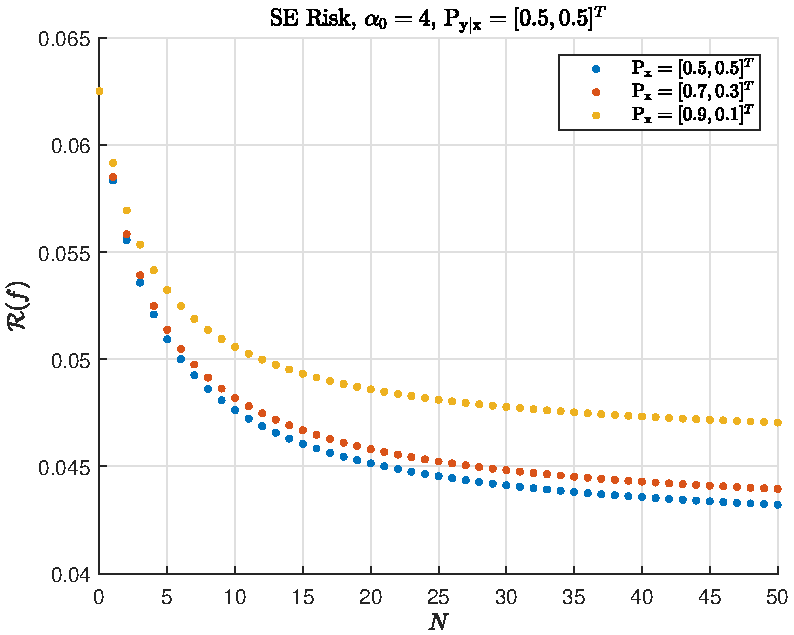
\includegraphics[scale=1.0]{Risk_SE_Dir_IO_N_leg_Px.pdf}
\caption{Optimal Squared-Error Risk vs $N$}
\label{fig:Risk_SE_Dir_IO_N_leg_Px}
\end{figure}

\begin{figure}
\centering
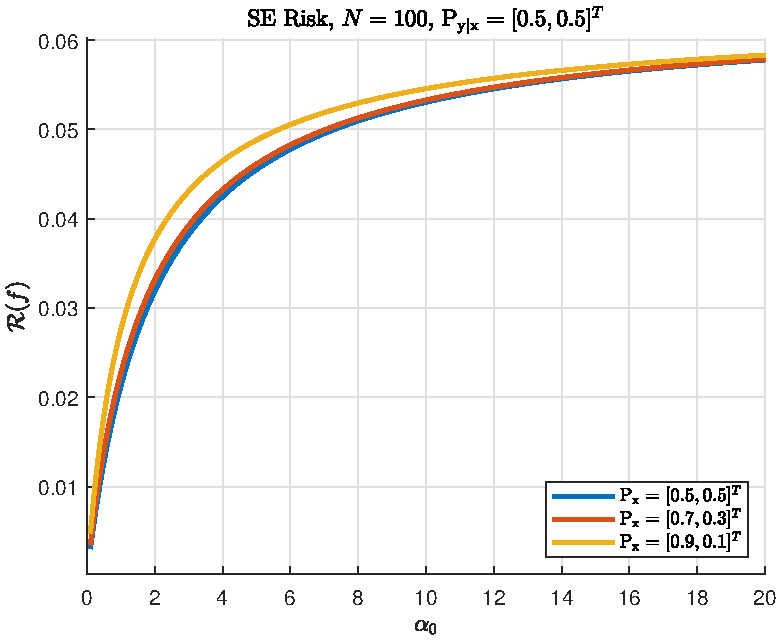
\includegraphics[scale=1.0]{Risk_SE_Dir_IO_a0_leg_Px.pdf}
\caption{Optimal Squared-Error Risk vs $\alpha_0$}
\label{fig:Risk_SE_Dir_IO_a0_leg_Px}
\end{figure}

\begin{figure}
\centering
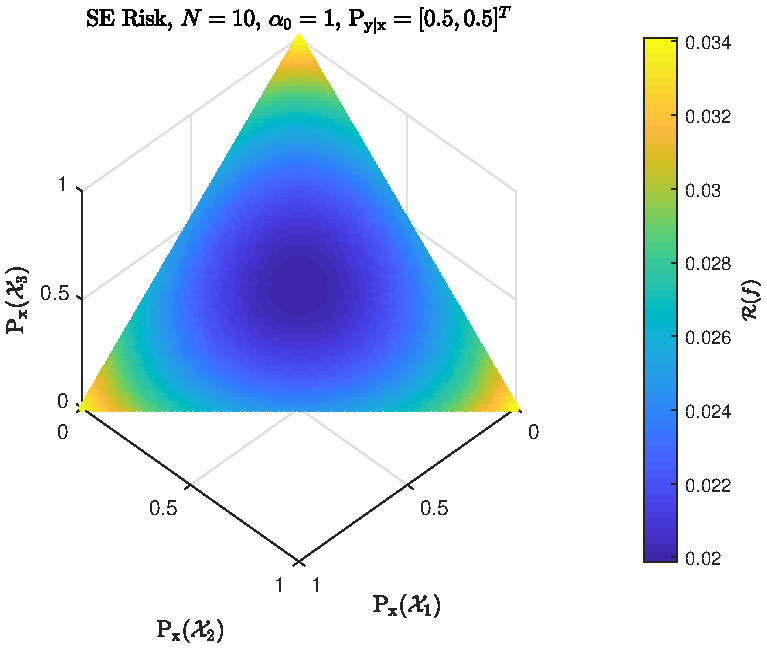
\includegraphics[scale=1.0]{Risk_SE_Dir_IO_Px_N_10_a0_1.pdf}
\caption{Optimal Squared-Error Risk vs $\text{P}(x)$}
\label{fig:Risk_SE_Dir_IO_Px_N_10_a0_1}
\end{figure}















\chapter{Extention to Dirichlet Prior}


\section{Intro}

PGR: Incomplete

PGR: Discuss distributions for alpha0 limits??? Trend toward impulses at mean or at Euclidean basis vectors?















\chapter{Extention to Infinite-Dimensional Spaces - Countably Infinite}


\section{Intro}

This chapter extends previous results for applications where the space $\Ycal$ can have an infinite number of elements. Specifically, the model distribution will be determined by using a Dirichlet random process prior. First, we assume that the set is countably infinite, that is $|\Ycal| = |\mathbb{N}|$; the model distribution is thus a discrete random process. 




\section{Basic Model}


\subsection{Objective}

PGR: ditto???


\subsection{Probability Distributions}

PGR: ???


\subsubsection{Model PDF, $\text{p}(\bm{\theta})$}

PGR: Valid model representation? Marginals instead?


\begin{IEEEeqnarray}{rCl}
\text{p}(\bm{\theta}) & = & \beta(\bm{\alpha})^{-1} \prod_{y \in \Ycal} \theta(y)^{\alpha(y) - 1} \;,
\end{IEEEeqnarray}

\begin{equation}
\beta(\bm{\alpha}) = \frac{\prod_{y \in \Ycal} \Gamma\big( \alpha(y) \big)}{\Gamma \left( \sum_{y \in \Ycal} \alpha(y) \right)} \;.
\end{equation}

The first and second joint moments of the model are 
\begin{equation}
\mu_{\theta}(y) = \text{E}\big[ \theta(y) \big] = \frac{\alpha(y)}{\alpha_0}
\end{equation}
and
\begin{IEEEeqnarray}{rCl}
\text{E} \big[ \theta(y) \theta(y') \big] & = & \frac{\alpha(y) \alpha(y') + \alpha(y) \delta[y,y']}{\alpha_0 (\alpha_0+1)} \;.
\end{IEEEeqnarray}




\subsubsection{Training Data PMF, $\text{P}(\Drm)$}

\begin{equation}
\text{P}(\Drm | \bm{\theta}) = \prod_{y \in \Ycal} \theta(y)^{\bar{N}(y;\Drm)} \;.
\end{equation}

\begin{equation}
\text{P}(\nbarrm | \bm{\theta}) = \mathcal{C}(\nbarrm) \prod_{y \in \Ycal} \theta(y)^{\bar{\nrm}(y)} \;,
\end{equation}

We extend the notion of the multinomial coefficient for general functions $\Ycal \mapsto \mathbb{N}$, such that 
\begin{equation}
\mathcal{C}(\bar{\bm{n}}) = \frac{\left( \sum_{y \in \Ycal} \bar{n}(y) \right)!}{\prod_{y \in \Ycal} \bar{n}(y)!} \;.
\end{equation}

Thus,
\begin{IEEEeqnarray}{rCl}
\text{P}(\nbarrm) & = & \mathcal{C}(\nbarrm) \beta(\bm{\alpha})^{-1} \beta(\bm{\alpha} + \nbarrm) \;.
\end{IEEEeqnarray}

The first and second joint moments of $\nbarrm$ are
\begin{equation}
\text{E}\big[ \bar{\nrm}(y) \big] = N \frac{\alpha(y)}{\alpha_0}
\end{equation}
and
\begin{equation}
\text{E}\big[ \bar{\nrm}(y) \bar{\nrm}(y') \big] 
= \frac{N}{\alpha_0 (\alpha_0+1)} \big( (\alpha_0 + N)\alpha(y) \delta[y,y'] + (N-1) \alpha(y) \alpha(y') \big) \;.
\end{equation}

Also,
\begin{equation}
\text{P}(\Drm) = \beta(\bm{\alpha})^{-1} \beta \big( \bm{\alpha} + \bar{\bm{N}}(\Drm) \big) \;.
\end{equation}






\subsubsection{Output conditional PMF, $\text{P}(\yrm | \Drm)$}

\begin{IEEEeqnarray}{rCL}
\text{p}(\bm{\theta} | \Drm) & = & \frac{\text{P}(\Drm | \bm{\theta}) \text{p}(\bm{\theta})}{\text{P}(\Drm)} \\
& = & \beta \left( \bm{\alpha} + \bar{\bm{N}}(\Drm) \right)^{-1} \prod_{y \in \Ycal} \theta(y)^{\alpha(y) + \bar{N}(y;\Drm) - 1} \nonumber 
\end{IEEEeqnarray}

\begin{IEEEeqnarray}{rCL}
\text{p}(\bm{\theta} | \nbarrm) = \beta \left( \bm{\alpha} + \nbarrm \right)^{-1} 
\prod_{y \in \Ycal} \theta(y)^{\alpha(y) + \bar{\nrm}(y) - 1} \;,
\end{IEEEeqnarray}

The PMF of interest is
\begin{IEEEeqnarray}{rCl}
\text{P}(\yrm | \Drm) & = & \text{E}_{\bm{\theta} | \Drm}\big[ \theta(\yrm) | \Drm \big] \\
& = & \frac{\alpha(\yrm) + \bar{N}(\yrm;\Drm)}{\alpha_0 + N} \nonumber \\
& = & \left(\frac{\alpha_0}{\alpha_0+N}\right) \frac{\alpha(\yrm)}{\alpha_0} + \left(\frac{N}{\alpha_0+N}\right) \frac{\bar{N}(\yrm;\Drm)}{N} \nonumber
\end{IEEEeqnarray}

\begin{IEEEeqnarray}{rCl}
\text{P}(\yrm | \nbarrm) & = & \text{E}_{\bm{\theta} | \nbarrm} \big[ \theta(\yrm) | \nbarrm \big] \\
& = & \frac{\alpha(\yrm) + \bar{\nrm}(\yrm)}{\alpha_0 + N} \nonumber \\
& = & \left(\frac{\alpha_0}{\alpha_0+N}\right) \frac{\alpha(\yrm)}{\alpha_0} + \left(\frac{N}{\alpha_0+N}\right) \frac{\bar{\nrm}(\yrm)}{N} \nonumber
\end{IEEEeqnarray}



\section{Application to Common Loss Functions}

PGR: Definitely regression. Classification sensible for countably infinite?

PGR: Results identical to finite Dirichlet

\begin{IEEEeqnarray}{L}
\text{E}_{\yrm | \Drm} \big[ \mathcal{L}(h,\yrm) \big] = \sum_{y \in \Ycal} \mathcal{L}(h,y) \text{P}_{\yrm | \Drm}(y | \Drm) \\
= \frac{\sum_{y \in \Ycal} \alpha(y) \mathcal{L}(h,y) + \sum_{y \in \Ycal} \bar{N}(y;\Drm) \mathcal{L}(h,y)}{\alpha_0+N} \nonumber \\
= \frac{\sum_{y \in \Ycal} \alpha(y) \mathcal{L}(h,y) + \sum_{n=1}^N \mathcal{L}\big( h,\Drm(n) \big)}{\alpha_0+N} \nonumber \\
= \left( \frac{\alpha_0}{\alpha_0+N} \right) \sum_{y \in \Ycal} \mathcal{L}(h,y) \frac{\alpha(y)}{\alpha_0} +  \left( \frac{N}{\alpha_0+N} \right) N^{-1} \sum_{n=1}^N \mathcal{L}\big( h,\Drm(n) \big) \nonumber \;.
\end{IEEEeqnarray}


\section{General Model}

Extension to output and input spaces $\Ycal$ and $\Xcal$ can have an infinite number of elements. 


\section{Applications: General Model}

PGR: Definitely regression. Classification sensible for countably infinite?

PGR: Results identical to finite Dirichlet












\chapter{Extention to Infinite-Dimensional Spaces - Uncountably Infinite}

PGR: account for impulsive alpha?


\section{Intro}

This chapter extends further to the case where $\Ycal$ is countably infinite, that is $|\Ycal| > |\mathbb{N}|$; the model distribution is thus a continuous random process. 


\section{Basic Model}


\subsection{Objective}

PGR: ditto???


\subsection{Probability Distributions}

PGR: ???


\subsubsection{Model $\theta$ Characterization}

The model is now a continuous random process, such that $\theta \sim \text{DP}(\alpha)$. The concentration parameter is $\alpha_0 = \int_{y \in \Ycal} \alpha(y) \mathrm{d} y$. By definition, for any partition of the set $\Ycal$, $\left\{ \ldots,S(z),\ldots \right\}$, $z \in \Zcal$, we can generate a discrete Dirichlet random vector/process $\phi(z) \equiv \int_{S(z)} \theta(y) \mathrm{d} y$ with parameterizing function $\lambda(z) \equiv \int_{S(z)} \alpha(y) \mathrm{d} y$. This is commonly referred to as the aggregation property. The PDF for the aggregation is thus
\begin{IEEEeqnarray}{rCl}
\text{p}(\phi) & = & \beta(\lambda)^{-1} \prod_{z \in \Zcal} \phi(z)^{\lambda(z) - 1} \;.
\end{IEEEeqnarray}

As detailed in Appendix \ref{app:E_DP}, the first and second moments of a Dirichlet process $\text{DP}(\alpha)$ are
\begin{equation}
\mu_{\theta}(y) = \text{E}\big[\theta(y)\big] = \frac{\alpha(y)}{\alpha_0}
\end{equation}
and
\begin{IEEEeqnarray}{rCl}
\text{E} \big[ \theta(y) \theta(y') \big] & = & \frac{\alpha(y) \alpha(y') + \alpha(y) \delta(y-y')}{\alpha_0 (\alpha_0+1)} \;.
\end{IEEEeqnarray}







\subsubsection{Output conditional PDF, $\text{p}(\yrm | \Drm)$}

In Appendix \ref{app:DP_post}, it was shown that if the model $\theta \sim \text{DP}(\alpha)$ is a Dirichlet process, then the model conditioned on the training data $\Drm$ is also a Dirichlet process with parameterizing function $\alpha(\cdot) + \bar{N}(\cdot;\Drm)$, where $\bar{N}(y;\Drm) = \sum_{n=1}^N \delta\left( y - \Drm(n) \right)$ generalizes from the discrete case. Thus, the conditional PDF of interest can be formulated as
\begin{IEEEeqnarray}{rCl}
\text{p}(\yrm | \Drm) & = & \text{E}_{\bm{\theta} | \Drm}\big[ \theta(\yrm) | \Drm \big] \\
& = & \frac{\alpha(\yrm) + \sum_{n=1}^N \delta\big( \yrm - \Drm(n) \big)}{\alpha_0 + N} \nonumber \\
& = & \left(\frac{\alpha_0}{\alpha_0+N}\right) \frac{\alpha(\yrm)}{\alpha_0} + \left(\frac{N}{\alpha_0+N}\right) \frac{\sum_{n=1}^N \delta\big( \yrm - \Drm(n) \big)}{N} \nonumber \\
& = & \frac{\alpha(\yrm) + \bar{N}(\yrm;\Drm)}{\alpha_0 + N} \nonumber \;.
\end{IEEEeqnarray}

With the generalization to a continuous set $\Ycal$, the training data dependent component of the PDF is formulated with Dirac delta functions. 



\subsubsection{Training Data PDF, $\text{p}(\Drm)$}

To represent the training data distribution, note that the Dirichlet process conditional model also provides
\begin{IEEEeqnarray}{rCl}
\text{p}\big( \Drm(n+1) | \Drm(n),\ldots,\Drm(1) \big) & = & \frac{\alpha\big( \Drm(n+1) \big) + \sum_{n'=1}^N \delta\big( \Drm(n+1) - \Drm(n') \big)}{\alpha_0 + N} \;
\end{IEEEeqnarray}
and thus the complete PDF is
\begin{IEEEeqnarray}{rCl}
\text{p}(\Drm) & = & \text{p}\big( \Drm(1) \big) \prod_{n=2}^N \text{p}\big( \Drm(n) | \Drm(n-1),\ldots,\Drm(1) \big) \\
& = & \frac{\alpha\big( \Drm(1) \big)}{\alpha_0} \prod_{n=2}^N \frac{\alpha\big( \Drm(n) \big) + \sum_{i=1}^{n-1} \delta\big( \Drm(n)-\Drm(i) \big)}{\alpha_0+n-1} \nonumber \;.
\end{IEEEeqnarray}

Additionally, note that since $\text{p}_{\Drm(n) | \theta}(y|\theta) = \theta(y)$ is independent of sample index $n$, the PDF does not vary when the input arguments are permuted. Furthermore, all marginal distributions of $\Drm$ will have the same form, regardless of which training samples $\Drm(n)$ are used.

Using these properties, the first and second joint moments of $\Drm$ are found to be
\begin{IEEEeqnarray}{rCl}
\text{E}\big[ \Drm(n) \big] & = & \int_{\Ycal} y \text{p}_{\Drm(n)}(y) \mathrm{d} y = \int_{\Ycal} y \text{E}_{\bm{\theta}}\big[ \text{P}_{\Drm(n) | \bm{\theta}}(y) \big] \mathrm{d} y \\
& = & \int_{\Ycal} y \text{E}_{\bm{\theta}}\big[ \theta(y) \big] \mathrm{d}y \nonumber \\
& = & \int_{\Ycal} y \frac{\alpha(y)}{\alpha_0} \mathrm{d} y \equiv \mu_{\yrm} \nonumber
\end{IEEEeqnarray}
and
\begin{IEEEeqnarray}{rCl}
\text{E}\big[ \Drm(n)^2 \big] & = & \int_{\Ycal} y^2 \text{p}_{\Drm(n)}(y) \mathrm{d} y = \int_{\Ycal} y^2 \text{E}_{\bm{\theta}}\big[ \text{P}_{\Drm(n) | \bm{\theta}}(y) \big] \mathrm{d}y \\
& = & \int_{\Ycal} y^2 \text{E}_{\bm{\theta}}\big[ \theta(y) \big] \mathrm{d}y \nonumber \\
& = & \int_{\Ycal} y^2 \frac{\alpha(y)}{\alpha_0} \mathrm{d}y = \text{E}[\yrm^2] \nonumber \;,
\end{IEEEeqnarray}

\begin{IEEEeqnarray}{rCl}
\text{E}\big[ \Drm(n)\Drm(n') \big] & = & \int_{\Ycal} \int_{\Ycal} y y' \text{p}_{\Drm(n),\Drm(n')}(y,y') \mathrm{d} y \mathrm{d}y' \\
& = & \int_{\Ycal} \int_{\Ycal} y y' \text{E}_{\bm{\theta}} \big[ \text{p}_{\Drm(n) | \bm{\theta}}(y) \text{p}_{\Drm(n') | \bm{\theta}}(y') \big] \mathrm{d}y \mathrm{d}y' \nonumber \\
& = & \int_{\Ycal} \int_{\Ycal} y y' \text{E}_{\bm{\theta}}\big[ \theta(y) \theta(y') \big] \mathrm{d}y \mathrm{d}y' \nonumber \\
& = & \int_{\Ycal} \int_{\Ycal} y y' \frac{\alpha(y) \alpha(y') + \alpha(y) \delta(y-y')}{\alpha_0 (\alpha_0+1)} \mathrm{d}y \mathrm{d}y' \nonumber \\
& = & \frac{\alpha_0 \mu_{\yrm}^2 + \text{E}[\yrm^2]}{\alpha_0 + 1} \nonumber \;.
\end{IEEEeqnarray}

Combining,
\begin{equation}
\text{E}\big[ \Drm(n)\Drm(n') \big] = \text{E}[\yrm^2] - \big(1 - \delta[n,n']\big) \frac{\alpha_0}{\alpha_0+1} \Sigma_{\yrm} \;.
\end{equation}

PGR: move proofs to appendix???


PGR PGR: Dirichlet-Multinomial Process perspective???

Define the Dirichlet-Multinomial process $\bar{\nrm}(\cdot) \equiv \bar{N}(\cdot;\Drm)$. The mean and correlation functions below are found in Appendix \ref{app:DMP}. The mean function is
\begin{IEEEeqnarray}{rCl}
\text{E}\big[ \bar{\nrm}(y) \big] & = & N \frac{\alpha(y)}{\alpha_0} 
\end{IEEEeqnarray}
and the correlation function is
\begin{IEEEeqnarray}{rCl}
\text{E}\big[ \bar{\nrm}(y) \bar{\nrm}(y') \big] & = & \frac{N}{\alpha_0 (\alpha_0+1)} \big[ (N-1)\alpha(y) \alpha(y') + (\alpha_0+N) \alpha(y) \delta(y-y') \big] \;.
\end{IEEEeqnarray}




\section{Application to Common Loss Functions}

PGR: Discuss continuous notation

\begin{IEEEeqnarray}{L}
\text{E}_{\yrm | \Drm} \big[ \mathcal{L}(h,\yrm) \big] = \int_{\Ycal} \mathcal{L}(h,y) \text{p}_{\yrm | \Drm}(y | \Drm) \mathrm{d}y \\
= \frac{\int_{\Ycal} \alpha(y) \mathcal{L}(h,y) \mathrm{d} y + \int_{\Ycal} \sum_{n=1}^N \delta\big( y-\Drm(n) \big) \mathcal{L}(h,y) \mathrm{d} y}{\alpha_0+N} \nonumber \\
= \frac{\int_{\Ycal} \alpha(y) \mathcal{L}(h,y) \mathrm{d} y + \sum_{n=1}^N \mathcal{L}\big( h,\Drm(n) \big)}{\alpha_0+N} \nonumber \\
= \left( \frac{\alpha_0}{\alpha_0+N} \right) \int_{\Ycal} \frac{\alpha(y)}{\alpha_0} \mathcal{L}(h,y) \mathrm{d}y +  \left( \frac{N}{\alpha_0+N} \right) N^{-1} \sum_{n=1}^N \mathcal{L}\big( h,\Drm(n) \big) \nonumber 
\end{IEEEeqnarray}


\subsection{Regression: the Squared-Error Loss}

\begin{equation}
\mathcal{L}(h,y) = (h-y)^2 \;.
\end{equation}

Now we choose for the regression function to map to $\Hcal = \Ycal = \mathbb{R}$.

\begin{IEEEeqnarray}{rCl}
\mathcal{R}(f) & = & \text{E}_{\bm{\theta}} \Bigg[ \text{E}_{\Drm | \bm{\theta}} \bigg[ \text{E}_{\yrm | \bm{\theta}} \Big[ \big( f(\Drm)-\yrm \big)^2 \Big] \bigg] \Bigg] \\
& = & \text{E}_{\bm{\theta}} \Big[ \text{E}_{\yrm | \bm{\theta}} \big[ (\yrm - \mu_{\yrm | \bm{\theta}})^2 \big] \Big] + \text{E}_{\bm{\theta}} \bigg[ \text{E}_{\Drm | \bm{\theta}} \Big[ \big( f(\Drm) - \mu_{\yrm | \bm{\theta}} \big)^2 \Big] \bigg] \nonumber \\
& = & \text{E}_{\bm{\theta}} \left[ \Sigma_{\yrm | \bm{\theta}} \right] + \text{E}_{\bm{\theta}} \bigg[ \text{E}_{\Drm | \bm{\theta}} \Big[ \big( f(\Drm) - \mu_{\yrm | \bm{\theta}} \big)^2 \Big] \bigg] \nonumber
\end{IEEEeqnarray}


\subsubsection{Optimal Learner}

The optimal function is again the expected value of the output conditional PMF,
\begin{IEEEeqnarray}{rCl}
f^*(\Drm) & = & \argmin_{h \in \mathbb{R}} \text{E}_{\yrm | \Drm} \big[ (h-\yrm)^2 \big]  \\
& = & \mu_{\yrm | \Drm} = \text{E}_{\bm{\theta} | \Drm} [ \mu_{\yrm | \bm{\theta}} ] \nonumber \\
& = & \left( \frac{\alpha_0}{\alpha_0+N} \right) \int_{\Ycal} \frac{\alpha(y)}{\alpha_0} y \mathrm{d}y +  \left( \frac{N}{\alpha_0+N} \right) \frac{1}{N} \sum_{n=1}^N \Drm(n) \nonumber \\
& = & \left( \frac{\alpha_0}{\alpha_0+N} \right) \text{E}[\yrm] +  \left( \frac{N}{\alpha_0+N} \right) \frac{1}{N} \sum_{n=1}^N \Drm(n) \nonumber \\
& = & \left( \frac{\alpha_0}{\alpha_0+N} \right) \mu_{\yrm} +  \left( \frac{N}{\alpha_0+N} \right) \int_{\Ycal} y \frac{\bar{N}(y;\Drm)}{N} \mathrm{d}y \nonumber \;.
\end{IEEEeqnarray}




\subsubsection{Minimum Risk}

\begin{IEEEeqnarray}{rCl}
\mathcal{R}(f^*) & = & \text{E}_{\Drm} \left[ \Sigma_{\yrm | \Drm} \right] \\
& = & \text{E}_{\bm{\theta}} \left[ \Sigma_{\yrm | \bm{\theta}} \right] + \text{E}_{\Drm} \bigg[ \text{E}_{\bm{\theta} | \Drm} \Big[ \big( \mu_{\yrm | \bm{\theta}} - \text{E}_{\bm{\theta} | \Drm}[\mu_{\yrm | \bm{\theta}}] \big)^2 \Big] \bigg] \nonumber \\
& = & \text{E}_{\bm{\theta}} \left[ \Sigma_{\yrm | \bm{\theta}} \right] + \text{E}_{\Drm} \big[ \text{C}_{\bm{\theta} | \Drm} [ \mu_{\yrm | \bm{\theta}} ] \big] \nonumber \\
& = & \text{E}_{\nbarrm} \left[ \Sigma_{\yrm | \nbarrm} \right] \nonumber \;.
\end{IEEEeqnarray}


The conditional variance is expanded as
\begin{IEEEeqnarray}{rCl}
\Sigma_{\yrm | \Drm} & = & \text{E}_{\yrm | \Drm}[\yrm^2]
- \big( \text{E}_{\yrm | \Drm}[\yrm] \big)^2 
\end{IEEEeqnarray}
and the expectations of the two terms are evaluated separately.


\begin{IEEEeqnarray}{rCl}
\text{E}_{\Drm}\big[\text{E}_{\yrm | \Drm}[\yrm^2]\big] & = & \text{E}_{\yrm}[\yrm^2]
\end{IEEEeqnarray}


\begin{IEEEeqnarray}{L}
\text{E}_{\Drm}\Big[ \big( \text{E}_{\yrm | \Drm}[\yrm] \big)^2 \Big] \\
\quad = \frac{\alpha_0^2 \mu_{\yrm}^2 + 2\alpha_0 \mu_{\yrm} \sum_{n=1}^N \text{E}\big[ \Drm(n) \big] + \sum_{n=1}^N \sum_{n'=1}^N \text{E}\big[ \Drm(n)\Drm(n') \big]}{(\alpha_0+N)^2} \nonumber \\
\quad = \frac{\alpha_0^2 \mu_{\yrm}^2 + 2\alpha_0 N \mu_{\yrm}^2 + N^2\text{E}[\yrm^2] - N(N-1)\alpha_0(\alpha_0+1)^{-1} \Sigma_{\yrm}}{(\alpha_0+N)^2} \nonumber \\
\quad = \mu_{\yrm}^2 + \frac{N^2 - N(N-1)\alpha_0(\alpha_0+1)^{-1}}{(\alpha_0+N)^2} \Sigma_{\yrm} \nonumber
\end{IEEEeqnarray}

PGR: DMP PERSPECTIVE???

\begin{IEEEeqnarray}{L}
\text{E}_{\Drm}\Big[ \big( \text{E}_{\yrm | \Drm}[\yrm] \big)^2 \Big] = \text{E}_{\bar{\nrm}}\Big[ \big( \text{E}_{\yrm | \bar{\nrm}}[\yrm] \big)^2 \Big] \\
\quad = \frac{\alpha_0^2 \mu_{\yrm}^2 + 2\alpha_0 \mu_{\yrm} \int_{\Ycal} y \text{E}\big[ \bar{\nrm}(y) \big] \mathrm{d}y + \int_{\Ycal} \int_{\Ycal} y y'\text{E}\big[ \bar{\nrm}(y)\bar{\nrm}(y') \big] \mathrm{d}y \mathrm{d}y'}{(\alpha_0+N)^2} \nonumber \\
\quad = \frac{\alpha_0^2 \mu_{\yrm}^2 + 2\alpha_0 N \mu_{\yrm}^2 + N(N-1)\alpha_0(\alpha_0+1)^{-1} \mu_{\yrm}^2 + N(\alpha_0+N)(\alpha_0+1)^{-1}\text{E}[\yrm^2]}{(\alpha_0+N)^2} \nonumber \\
\quad = \frac{\alpha_0(\alpha_0+N+1)\mu_{\yrm}^2 + N\text{E}[\yrm^2]}{(\alpha_0+1)(\alpha_0+N)} \nonumber
\end{IEEEeqnarray}

PGR: nicer algebra with DMP!

PGR: DMP


The optimal risk is again

\begin{IEEEeqnarray}{rCl}
\mathcal{R}(f^*) & = & \left( 1 - \frac{N^2 - N(N-1)\alpha_0(\alpha_0+1)^{-1}}{(\alpha_0+N)^2} \right) \Sigma_{\yrm} \\
& = & \frac{\alpha_0 (\alpha_0+N+1)}{(\alpha_0+1)(\alpha_0+N)} \Sigma_{\yrm} \nonumber \\
& = & \frac{1+(\alpha_0+N)^{-1}}{1+\alpha_0^{-1}} \Sigma_{\yrm} \nonumber \;.
\end{IEEEeqnarray}

As for finite Dirichlet models and discrete Dirichlet processes, the optimal risk is dependent on the model only through the concentration parameter $\alpha_0$ and the variance of the expected distribution $\text{P}(\yrm) = \text{E}_{\theta}\big[ \theta(\yrm) ]$.




\section{General Model}

PGR: change dirac deltas to kronecker in fractions, no divide by zero???

\subsection{Model Extension}

This section adds the input space $\Xcal$, now considered to be countably infinite; that is $|\Xcal| > |\mathbb{N}|$. The model distribution is a random process over the space $\Ycal \times \Xcal$.


\subsection{General Probability Distributions}

PGR


\subsubsection{Model $\theta$ Characterization}

The model random process is now defined over the set $\Ycal \times \Xcal$; this Dirichlet process is defined as $\theta \sim \text{DP}(\alpha)$ with $\alpha : \Ycal \times \Xcal \mapsto \mathbb{R}_{>0}$. The concentration parameter generalizes to $\alpha_0 = \int_{\Ycal} \int_{\Xcal} \alpha(y,x) \mathrm{d} x \mathrm{d} y$. Using the aggregation property, any partition of the set $\Ycal \times \Xcal$, $\left\{ \ldots,S(z),\ldots \right\}$, $z \in \Zcal$ is a discrete Dirichlet random vector/process $\phi(z) = \iint_{S(z)} \theta(y,x) \mathrm{d} x \mathrm{d} y$ with parameterizing function $\lambda(z) = \iint_{S(z)} \alpha(y,x) \mathrm{d} x \mathrm{d} y$. The PDF for the aggregation is
\begin{IEEEeqnarray}{rCl}
\text{p}(\phi) & = & \beta(\lambda)^{-1} \prod_{z \in \Zcal} \phi(z)^{\lambda(z) - 1} \;.
\end{IEEEeqnarray}

The expected value of a Dirichlet process generalizes to $\text{DP}(\alpha)$
\begin{equation}
\mu_{\theta}(y,x) = \text{E}\big[ \theta(y,x) \big] = \frac{\alpha(y,x)}{\alpha_0}
\end{equation}
and the correlation function is
\begin{IEEEeqnarray}{rCl}
\text{E} \big[ \theta(y,x) \theta(y',x') \big] & = & \frac{\alpha(y,x) \alpha(y',x') + \alpha(y,x) \delta(y-y')\delta(x-x')}{\alpha_0 (\alpha_0+1)} \;.
\end{IEEEeqnarray}






\subsubsection{Output conditional PDF, $\text{p}(\yrm | \xrm,\Drm)$}

The properties of the Dirichlet distribution proven in Appendix \ref{app:DP_post} generalize, such that the model conditioned on the training data $\Drm$ is Dirichlet with parameterizing function $\alpha(y,x) + \bar{N}(y,x;\Drm)$, where $\bar{N}(y,x;\Drm) = \sum_{n=1}^N \delta\left( y - \Yrm(n) \right)\left( x - \Xrm(n) \right)$. Recall that $\Drm(n) = \big( \Yrm(n),\Xrm(n) \big)$ with $Y \in \Ycal^N$ and $X \in \Xcal^N$.

The PDF $\text{p}(\yrm,\xrm | \Drm)$ is thus
\begin{IEEEeqnarray}{rCl}
\text{p}(\yrm,\xrm | \Drm) & = & \text{E}_{\bm{\theta} | \Drm}\big[ \theta(\yrm,\xrm) | \Drm \big] \\
& = & \frac{\alpha(\yrm,\xrm) + \bar{N}(\yrm,\xrm;\Drm)}{\alpha_0 + N} \nonumber \\
& = & \frac{\alpha(\yrm,\xrm) + \sum_{n=1}^N \delta\big( \yrm - \Yrm(n) \big)\delta\big( \xrm - \Xrm(n) \big)}{\alpha_0 + N} \nonumber \\
& = & \left(\frac{\alpha_0}{\alpha_0+N}\right) \frac{\alpha(\yrm,\xrm)}{\alpha_0} + \left(\frac{N}{\alpha_0+N}\right) \frac{\sum_{n=1}^N \delta\big( \yrm - \Yrm(n) \big) \delta\big( \xrm - \Xrm(n) \big)}{N} \nonumber
\end{IEEEeqnarray}
and the conditional PDF of interest is
\begin{IEEEeqnarray}{rCl}
\text{p}(\yrm | \xrm,\Drm) & = & \frac{\alpha(\yrm,\xrm) + \bar{N}(\yrm,\xrm;\Drm)}{\alpha'(\xrm) + N'(\xrm;\Drm)} \\
& = & \frac{\alpha(\yrm,\xrm) + \sum_{n=1}^N \delta\big( \yrm - \Yrm(n) \big) \delta\big( \xrm - \Xrm(n) \big)}{\alpha'(\xrm) + \sum_{n=1}^N \delta\big( \xrm - X(n) \big)} \nonumber \\
& = & \left(\frac{\alpha'(\xrm)}{\alpha'(\xrm)+N'(\xrm;\Drm)}\right) \frac{\alpha(\yrm,\xrm)}{\alpha'(\xrm)} + \left(\frac{N'(\xrm;\Drm)}{\alpha'(\xrm)+N'(\xrm;\Drm)}\right) \frac{\bar{N}(\yrm,\xrm;\Drm)}{N'(\xrm;\Drm)} \nonumber \;,
\end{IEEEeqnarray}
where $\alpha'(x) = \int_{\Ycal} \alpha(y,x) \mathrm{d} y$ and $N'(x;\Drm) = \sum_{n=1}^N \delta\big( x - \Xrm(n) \big)$.

The conditional distribution for an uncountalbly infinite set $\Xcal$ has notable differences from its form for a countable input set. Specifically, as $N'(x;\Drm) \in [0,\infty)$, and in fact will either be zero or trend towards infinity, the coefficients dictating the convex combination of distributions will be zero or one (assuming a non-impulsive model parameter $\alpha$). Thus, the distribution for a given observation $\xrm$ will be either strictly dependent on either the training data or the prior knowledge regarding $\theta$.



\subsubsection{Training Data PDF, $\text{p}(\Drm)$}

By the Dirichlet process properties,
\begin{IEEEeqnarray}{L}
\text{p}\big( \Drm(n+1) | \Drm(n),\ldots,\Drm(1) \big) = \\
\quad \frac{\alpha\big( \Yrm(n+1),\Xrm(n+1) \big) + \sum_{n'=1}^N \delta\big( \Yrm(n+1) - \Yrm(n') \big) \delta\big( \Xrm(n+1) - \Xrm(n') \big)}{\alpha_0 + N} \nonumber
\end{IEEEeqnarray}
and thus
\begin{IEEEeqnarray}{rCl}
\text{p}(\Drm) & = & \text{p}\big (\Drm(1) \big) \prod_{n=2}^N \text{p}\big( \Drm(n) | \Drm(n-1),\ldots,\Drm(1) \big) \\
& = & \frac{\alpha\big( \Yrm(1),\Xrm(1) \big)}{\alpha_0} \prod_{n=2}^N \frac{\alpha\big( \Yrm(n),\Xrm(n) \big) + \sum_{i=1}^{n-1} \delta\big( \Yrm(n)-\Yrm(i) \big) \delta\big( \Xrm(n)-\Xrm(i) \big)}{\alpha_0+n-1} \nonumber
\end{IEEEeqnarray}

It is informative to find the PDF's for the training output values $\Yrm$ given the input values $\Xrm$, as well as the marginal PDF for the input values alone. Observe that the PDF for $\Xrm$ can be represented as
\begin{IEEEeqnarray}{rCl}
\text{p}(\Xrm) & = & \text{E}_{\theta}\big[ \text{p}(\Xrm | \theta) \big] = \text{E}_{\theta}\left[ \prod_{n=1}^N \theta'\big( \Xrm(n) \big) \right] \\
& = & \frac{\alpha'\big( \Xrm(1) \big)}{\alpha_0} \prod_{n=2}^N \frac{\alpha'\big( \Xrm(n) \big) + \sum_{i=1}^{n-1} \delta\big( \Xrm(n)-\Xrm(i) \big)}{\alpha_0+n-1} \nonumber
\end{IEEEeqnarray}
where, by the aggregation principle, $\theta'(x) = \int_{\Ycal} \theta(y,x) \mathrm{d} y$ is a Dirichlet process with parameter function $\alpha': \Xcal \mapsto \mathbb{R}_{>0}$.


%The PDF for $\Xrm$ is
%\begin{IEEEeqnarray}{rCl}
%\text{p}(X) & = & \int_{Y(1)} \mathrm{d}Y(1) \ldots \int_{Y(N)} \mathrm{d}Y(N) \frac{\alpha(Y(1),X(1))}{\alpha_0} \\
%&& \quad \prod_{n=2}^N \frac{\alpha(Y(n),X(n)) + \sum_{i=1}^{n-1} \delta(Y(n)-Y(i)) \delta(X(n)-X(i))}{\alpha_0+n-1} \\
%& = & \int_{Y(1)} \mathrm{d}Y(1) \ldots \int_{Y(N-1)} \mathrm{d}Y(N-1) \frac{\alpha(Y(1),X(1))}{\alpha_0} \\
%&& \quad \prod_{n=2}^{N-1} \frac{\alpha(Y(n),X(n)) + \sum_{i=1}^{n-1} \delta(Y(n)-Y(i)) \delta(X(n)-X(i))}{\alpha_0+n-1} \\
%&& \qquad \frac{\alpha'(X(N)) + \sum_{i=1}^{N-1} \delta(X(N)-X(i))}{\alpha_0+N-1} \\
%& = & \ldots \\
%& = & \frac{\alpha'(X(1))}{\alpha_0} \prod_{n=2}^N \frac{\alpha'(X(n)) + \sum_{i=1}^{n-1} \delta(X(n)-X(i))}{\alpha_0+n-1}
%\end{IEEEeqnarray}

Additionally, by the invariance principle, the PDF's for the first-degree marginals are
\begin{IEEEeqnarray}{rCl}
\text{p}\big( \Xrm(n) \big) & = & \frac{\alpha'\big( \Xrm(n) \big)}{\alpha_0} \;.
\end{IEEEeqnarray}
which necessarily have the same form as the PDF of the observed value $\xrm$.

The conditional distribution of intererest is
\begin{IEEEeqnarray}{rCl}
\text{p}(\Yrm | \Xrm) & = & \frac{\text{p}(\Yrm,\Xrm)}{\text{p}(\Xrm)} \\
& = & \frac{\alpha\big( \Yrm(1),\Xrm(1) \big)}{\alpha'\big( \Xrm(1) \big)} \prod_{n=2}^N \frac{\alpha\big( \Yrm(n),\Xrm(n) \big) + \sum_{i=1}^{n-1} \delta\big( \Yrm(n)-\Yrm(i) \big) \delta\big( \Xrm(n)-\Xrm(i) \big)}{\alpha'\big( \Xrm(n) \big) + \sum_{i=1}^{n-1} \delta\big( \Xrm(n)-\Xrm(i) \big)} \nonumber
\end{IEEEeqnarray}

Marginalized conditional PDF's for the first and second samples are found. Observe that the marginal distribution for the first $N-1$ values of $\Yrm$ is
\begin{IEEEeqnarray}{L}
\text{p}\big( \Yrm(1),\ldots,\Yrm(N-1) | \Xrm \big) \\
= \int_{\Ycal} \frac{\alpha\big( \Yrm(1),\Xrm(1) \big)}{\alpha'\big( \Xrm(1) \big)} \nonumber \\
\quad \prod_{n=2}^N \frac{\alpha
\big( \Yrm(n),\Xrm(n) \big) + \sum_{i=1}^{n-1} \delta\big( \Yrm(n)-\Yrm(i) \big) \delta\big( \Xrm(n)-\Xrm(i) \big)}{\alpha'\big( \Xrm(n) \big) + \sum_{i=1}^{n-1} \delta\big( \Xrm(n)-\Xrm(i) \big)} \mathrm{d}\Yrm(N) \nonumber \\
= \frac{\alpha\big( \Yrm(1),\Xrm(1) \big)}{\alpha'\big( \Xrm(1) \big)} \prod_{n=2}^{N-1} \frac{\alpha\big( \Yrm(n),\Xrm(n) \big) + \sum_{i=1}^{n-1} \delta\big( \Yrm(n)-\Yrm(i) \big) \delta\big( \Xrm(n)-\Xrm(i) \big)}{\alpha'\big( \Xrm(n) \big) + \sum_{i=1}^{n-1} \delta\big( \Xrm(n)-\Xrm(i) \big)} \nonumber
\end{IEEEeqnarray}
which is independent of $\Xrm(n)$. Repeated integrations and an application of the permutation invariance principle produce the first and second order conditional distributions
\begin{IEEEeqnarray}{rCl}
\text{P}_{\Yrm(n) | \Xrm(n)} (y | x) & = & \frac{\alpha(y,x)}{\alpha'(x)}
\end{IEEEeqnarray}
and
\begin{IEEEeqnarray}{L}
\text{P}_{\Yrm(n),\Yrm(n') | \Xrm(n),\Xrm(n')} (y,y' | x,x') \\
\quad = \frac{\alpha(y,x) \alpha(y',x') + \alpha(y,x) \delta(y-y') \delta(x-x')}{\alpha'(x) \alpha'(x') + \alpha'(x') \delta(x-x')} \nonumber
\end{IEEEeqnarray}
and the first and second order moments of interest,
\begin{equation}
\text{E}\big[ \Yrm(n) | \Xrm \big] = \mu_{\yrm|\xrm}\big( \Xrm(n) \big) \;,
\end{equation}
\begin{equation}
\text{E}\big[ \Yrm(n)^2 | \Xrm \big] = \text{E}\big[ \yrm^2 | \xrm \big] \big( \Xrm(n) \big) \;,
\end{equation}
and 
\begin{IEEEeqnarray}{rCl}
\text{E}\big[ \Yrm(n) \Yrm(n') | \Xrm \big] & = & \frac{\alpha'\big( \Xrm(n) \big) \mu_{\yrm|\xrm}\big( \Xrm(n) ) \mu_{\yrm|\xrm}\big (\Xrm(n') \big) + \text{E}\big[ \yrm^2 | \xrm \big] \big( \Xrm(n) \big) \delta\big( \Xrm(n) - \Xrm(n') \big)}{\alpha'\big( \Xrm(n) \big) + \delta\big( \Xrm(n) - \Xrm(n') \big)} \;.
\end{IEEEeqnarray}


PGR: formalize permutation invariance principle???

PGR: Add Y given X equations (with Betas) for discrete case in previous chapters?



PGR: Dirichlet-Multinomial Process perspective

We have the DMP $\bar{\nrm}(y,x) \equiv \bar{N}(y,x;\Drm)$ with mean and correlation functions
\begin{IEEEeqnarray}{rCl}
\text{E}\big[ \bar{\nrm}(y,x) \big] & = & N \frac{\alpha(y,x)}{\alpha_0} 
\end{IEEEeqnarray}
and
\begin{IEEEeqnarray}{rCl}
\text{E}\big[ \bar{\nrm}(y,x) \bar{\nrm}(y',x') \big] & = & \frac{N}{\alpha_0 (\alpha_0+1)} \big[ (N-1)\alpha(y,x) \alpha(y',x') + (\alpha_0+N) \alpha(y,x) \delta(y-y') \delta(x-x') \big]
\end{IEEEeqnarray}

Observe that by the aggregation principle, $\nrm'(x) = \int_{\Ycal} \bar{\nrm}(y,x) \mathrm{d}y \equiv \sum_{n=1}^N \delta\big( x-\Xrm(n) \big)$ is a DMP over the set $\Xcal$ with parametrizing function $\alpha' : \Xcal \mapsto \mathbb{R}_{>0}$.

Additionally, the 1-dimensional subsets conditioned on the marginalized DMP are characterized as

\begin{equation}
\frac{\bar{\nrm}(\cdot,x)}{\delta(0)} \Big| \nrm'(x) \sim \text{DMP}\left( \frac{\nrm'(x)}{\delta(0)},\frac{\alpha(\cdot,x)}{\delta(0)} \right)
\end{equation}

PGR: add proof???








\section{Applications: General Model}

PGR: COPIED, incomplete

\begin{IEEEeqnarray}{L}
\text{E}_{\yrm | \xrm,\Drm} \big[ \mathcal{L}(h,\yrm) \big] = \int_{\Ycal} \mathcal{L}(h,y) \text{p}_{\yrm | \xrm,\Drm}(y | \xrm,\Drm) \mathrm{d}y \\
= \frac{\int_{\Ycal} \alpha(y,\xrm) \mathcal{L}(h,y) \mathrm{d}y + \int_{\Ycal} \bar{N}(y,\xrm;\Drm) \mathcal{L}(h,y) \mathrm{d}y}{\alpha'(\xrm)+N'(\xrm;\Drm)} \nonumber \\
= \frac{\int_{\Ycal} \alpha(y,\xrm) \mathcal{L}(h,y) \mathrm{d}y + \sum_{n=1}^N \delta\big( \xrm-\Xrm(n) \big) \mathcal{L}\big( h,\Drm(n) \big)}{\alpha'(\xrm)+N'(\xrm;\Drm)} \nonumber \\
= \left(\frac{\alpha'(\xrm)}{\alpha'(\xrm) + N'(\xrm;\Drm)}\right) \text{E}_{\yrm | \xrm}\big[ \mathcal{L}(h,\yrm) \big] + \left(\frac{N'(\xrm;\Drm)}{\alpha'(\xrm) + N'(\xrm;\Drm)}\right) \frac{\sum_{n=1}^N \delta\big( \xrm-\Xrm(n) \big) \mathcal{L}\big( h,\Yrm(n) \big)}{\sum_{n=1}^N \delta\big( \xrm-\Xrm(n) \big)} \nonumber \;.
\end{IEEEeqnarray}



\subsection{Regression: the Squared-Error Loss}

\begin{equation}
\mathcal{L}(h,y) = (h-y)^2 \;.
\end{equation}

Now we choose for the regression function to map to $\Hcal = \Ycal = \mathbb{R}$.

\begin{IEEEeqnarray}{rCl}
\mathcal{R}(f) & = & \text{E}_{\bm{\theta}} \Bigg[ \text{E}_{\Drm | \bm{\theta}} \bigg[ \text{E}_{\yrm,\xrm | \bm{\theta}} \Big[ \big( f( xrm,\Drm)-\yrm \big)^2 \Big] \bigg] \Bigg] \\
& = & \text{E}_{\xrm,\bm{\theta}} \Big[ \text{E}_{\yrm | \xrm,\bm{\theta}} \big[ (\yrm - \mu_{\yrm | \xrm,\bm{\theta}})^2 \big] \Big] + \text{E}_{\bm{\theta}} \bigg[ \text{E}_{\xrm,\Drm | \bm{\theta}} \Big[ \big( f(\xrm,\Drm) - \mu_{\yrm | \xrm,\bm{\theta}} \big)^2 \Big] \bigg] \nonumber \\
& = & \text{E}_{\xrm,\bm{\theta}} \left[ \Sigma_{\yrm | \xrm,\bm{\theta}} \right] + \text{E}_{\bm{\theta}} \bigg[ \text{E}_{\xrm,\Drm | \bm{\theta}} \Big[ \big( f(\xrm,\Drm) - \mu_{\yrm | \xrm,\bm{\theta}} \big)^2 \Big] \bigg] \nonumber
\end{IEEEeqnarray}



\subsubsection{Optimal Learner}

The optimal function is the expected value of the output conditional PDF,
\begin{IEEEeqnarray}{rCl}
f^*(\xrm,\Drm) & = & \mu_{\yrm | \xrm,\Drm}  = \text{E}_{\bm{\theta} | \xrm,\Drm} \left[ \mu_{\yrm | \xrm,\bm{\theta}} \right] \\
& = & \frac{\int_{\Ycal} y \big( \alpha(y,\xrm) + \bar{N}(y,\xrm;\Drm) \big) \mathrm{d}y}{\alpha'(\xrm) + N'(\xrm;\Drm)} \nonumber \\
& = & \left( \frac{\alpha'(\xrm)}{\alpha'(\xrm) + N'(\xrm;\Drm)} \right) \int_{\Ycal} y \frac{\alpha(y,\xrm)}{\alpha'(\xrm)} \mathrm{d}y \nonumber \\
&& \quad + \left( \frac{N'(\xrm;\Drm)}{\alpha'(\xrm) + N'(\xrm;\Drm)} \right) \frac{\sum_{n=1}^N \delta\big( \xrm-\Xrm(n) \big) \Yrm(n)}{\sum_{n=1}^N \delta\big( \xrm-\Xrm(n) \big)} \nonumber \\
& = & \left( \frac{\alpha'(\xrm)}{\alpha'(\xrm) + N'(\xrm;\Drm)} \right) \mu_{\yrm | \xrm} \nonumber \\
&& \quad + \left( \frac{N'(\xrm;\Drm)}{\alpha'(\xrm) + N'(\xrm;\Drm)} \right) \frac{\sum_{n=1}^N \delta\big( \xrm-\Xrm(n) \big) \Yrm(n)}{\sum_{n=1}^N \delta\big( \xrm-\Xrm(n) \big)} \nonumber \;.
\end{IEEEeqnarray}



\subsubsection{Minimum Risk}

Generalizing from the basic model discussion, we again have
\begin{IEEEeqnarray}{rCl}
\mathcal{R}(f^*) & = & \text{E}_{\xrm,\Drm} \left[ \Sigma_{\yrm | \xrm,\Drm} \right]
= \text{E}_{\xrm,\bar{\nrm}} \left[ \Sigma_{\yrm | \xrm,\bar{\nrm}} \right] \\
& = & \text{E}_{\xrm,\bm{\theta}} \left[ \Sigma_{\yrm | \xrm,\bm{\theta}} \right] + \text{E}_{\xrm,\Drm} \Big[ \text{C}_{\bm{\theta} | \xrm,\Drm} \big[ \mu_{\yrm | \xrm,\bm{\theta}} \big] \Big] \nonumber \;,
\end{IEEEeqnarray}
where we choose to perform the expectation over $\bar{\nrm}$. 

The conditional varance is now
\begin{IEEEeqnarray}{rCl}
\Sigma_{\yrm | \xrm,\bar{\nrm}} & = & \text{E}_{\yrm | \xrm,\bar{\nrm}}\big[ \yrm^2 \big]
- \big( \text{E}_{\yrm | \xrm,\bar{\nrm}}[\yrm] \big)^2 \;.
\end{IEEEeqnarray}
and the two terms are independently evaluated.


\begin{IEEEeqnarray}{L}
\text{E}_{\xrm,\Drm}\big[ \text{E}_{\yrm | \xrm,\Drm}\big[ \yrm^2 \big] \big] = \text{E}_{\xrm,\bar{\nrm}}\Big[ \text{E}_{\yrm | \xrm,\bar{\nrm}}\big[ \yrm^2 \big] \Big] \\
\quad = \text{E}_{\yrm}[\yrm^2] = \int_{\Ycal} y^2 \int_{\Xcal} \frac{\alpha(y,x)}{\alpha_0} \mathrm{d} x \mathrm{d}y \nonumber \\
\quad = \text{E}_{\xrm}\big[ \text{E}_{\yrm | \xrm}[\yrm^2] \big] = \int_{\Xcal} \frac{\alpha'(x)}{\alpha_0} \int_{\Ycal} y^2 \frac{\alpha(y,x)}{\alpha'(x)} \mathrm{d} y \mathrm{d}x \nonumber \;.
\end{IEEEeqnarray}



PGR: D PERSPECTIVE

\begin{IEEEeqnarray}{L}
\text{E}_{\xrm,\Drm} \left[ \big( \text{E}_{\yrm | \xrm,\Drm}[\yrm] \big)^2 \right] \\
\quad = \int_{\Xcal} \int_{\Dcal} \text{p}_{\xrm,\Drm}(x,D) \left( \int_{\Ycal} y \text{p}_{\yrm | \xrm,\Drm}(y | x,D) \mathrm{d}y \right)^2 \mathrm{d}D \mathrm{d}x \nonumber \\
\quad = \int_{\Xcal} \text{E}_{\Drm} \left[ \int_{\Ycal} y \text{p}_{\yrm,\xrm | \Drm}(y,x | \Drm) \mathrm{d} y \int_{\Ycal} y' \text{p}_{\yrm |\xrm,\Drm}(y' | x,\Drm) \mathrm{d} y' \right] \mathrm{d}x \nonumber \\ 
\quad = \int_{\Xcal} \text{E}_{\Yrm,\Xrm} \left[ \frac{ \left( \alpha'(x) \mu_{\yrm | \xrm}(x) + \sum_{n=1}^N \Yrm(n) \delta\big( x - \Xrm(n) \big) \right)^2 }{(\alpha_0+N) \left(\alpha'(x) + \sum_{n=1}^N \delta\big( x - \Xrm(n) \big) \right)} \right] \mathrm{d}x \nonumber \\ 
\quad = \int_{\Xcal} \text{E}_{\Xrm} \left[ \frac{ \text{E}_{\Yrm | \Xrm} \left[ \left( \alpha'(x) \mu_{\yrm | \yrm}(x) + \sum_{n=1}^N \Yrm(n) \delta\big( x - \Xrm(n) \big) \right)^2 \right] }{(\alpha_0+N) \left(\alpha'(x) + \sum_{n=1}^N \delta\big( x - \Xrm(n) \big) \right)} \right] \mathrm{d}x \nonumber 
\end{IEEEeqnarray}

Evaluating the expectation over $\Yrm$ given $\Xrm$, we have
\begin{IEEEeqnarray}{L}
\text{E}_{\Yrm | \Xrm} \left[ \left( \alpha'(x) \mu_{\yrm | \xrm}(x) + \sum_{n=1}^N \Yrm(n) \delta\big( x - \Xrm(n) \big) \right)^2 \right] \\ 
= \alpha'(x)^2 \mu_{\yrm | \xrm}(x)^2 + 2\alpha'(x) \mu_{\yrm | \xrm}(x) \sum_{n=1}^N \mu_{\yrm | \xrm}\big( \Xrm(n) \big) \delta\big( x - \Xrm(n) \big) \nonumber \\
\quad + \sum_{n=1}^N \text{E}\big[ \yrm^2 | \xrm \big]\big( \Xrm(n) \big) \delta\big( x - \Xrm(n) \big)^2 \nonumber \\
\quad + \sum_{n \neq n'} \frac{\alpha'\big( \Xrm(n) \big) \mu_{\yrm | \xrm}\big(\Xrm(n) \big) \alpha'\big( \Xrm(n') \big) \mu_{\yrm | \xrm}\big( \Xrm(n') \big) + \alpha'\big( \Xrm(n) \big) \text{E}\big[ \yrm^2 | \xrm \big]\big( \Xrm(n) \big) \delta\big( \Xrm(n)-\Xrm(n') \big)}{\alpha'\big( \Xrm(n) \big) \alpha'\big( \Xrm(n') \big) + \alpha'\big( \Xrm(n) \big) \delta\big( \Xrm(n)-\Xrm(n') \big)} \nonumber \\
\qquad \delta\big( x - \Xrm(n) \big) \delta\big( x - \Xrm(n') \big) \nonumber \\
\ldots \nonumber \\
= \alpha'(x)^2 \mu_{\yrm | \xrm}(x)^2 + 2\alpha'(x) \mu_{\yrm | \xrm}(x)^2 \sum_{n=1}^N \delta\big( x - \Xrm(n) \big) + \text{E}\big[ \yrm^2 | \xrm \big](x) \sum_{n=1}^N \delta\big( x - \Xrm(n) \big)^2 \nonumber \\
\quad + \frac{\alpha'(x) \mu_{\yrm | \xrm}(x)^2 + \text{E}\big[ \yrm^2 | \xrm \big](x) \delta(0)}{\alpha'(x) + \delta(0)} \nonumber \\
\qquad \sum_{n \neq n'} \delta\big( x - \Xrm(n) \big) \delta\big( x - \Xrm(n') \big) \nonumber \\
\ldots \nonumber \\
= \frac{\alpha'(x) + \sum_{n=1}^N \delta\big( x-\Xrm(n) \big)}{\alpha'(x) + \delta(0)} \nonumber \\
\quad \left( \text{E}\big[ \yrm^2 | \xrm \big](x) \delta(0) \sum_{n=1}^N \delta\big( x-\Xrm(n) \big) + \alpha'(x) \mu_{\yrm | \xrm}(x)^2 \left( \alpha'(x) + \delta(0) + \sum_{n=1}^N \delta\big( x-\Xrm(n) \big) \right) \right) \nonumber
\end{IEEEeqnarray}


PGR: Y given X PDFs, moments??? In PDF section, or in Appendix?





Plugging,
\begin{IEEEeqnarray}{L}
\text{E}_{\xrm,\Drm} \Big[ \big( \text{E}_{\yrm | \xrm,\Drm}[\yrm] \big)^2 \Big] \\
\quad = \int_{\Xcal} \text{E}_{\Xrm} \left[ \frac{ \text{E}_{\Yrm | \Xrm} \left[ \left( \alpha'(x) \mu_{\yrm | \xrm}(x) + \sum_{n=1}^N \Yrm(n) \delta\big( x - \Xrm(n) \big) \right)^2 \right] }{(\alpha_0+N) \left(\alpha'(x) + \sum_{n=1}^N \delta\big( x - \Xrm(n) \big) \right)} \right] \mathrm{d}x \nonumber \\ 
\quad = \int_{\Xcal} \frac{ \text{E}_{\Xrm} \left[ \text{E}\big[ \yrm^2 | \xrm \big](x) \delta(0) \sum_{n=1}^N \delta\big( x-\Xrm(n) \big) + \alpha'(x) \mu_{\yrm | \xrm}(x)^2 \left( \alpha'(x) + \delta(0) + \sum_{n=1}^N \delta\big( x-\Xrm(n) \right) \big) \right] }{(\alpha_0+N) \big( \alpha'(x) + \delta(0) \big)} \mathrm{d}x \nonumber 
\end{IEEEeqnarray}

Evaluating the expectation over $\Xrm$,
\begin{IEEEeqnarray}{L}
\text{E}_{\Xrm} \left[ \text{E}\big[ \yrm^2 | \xrm \big](x) \delta(0) \sum_{n=1}^N \delta\big( x-\Xrm(n) \big) + \alpha'(x) \mu_{\yrm | \xrm}(x)^2 \left( \alpha'(x) + \delta(0) + \sum_{n=1}^N \delta\big( x-\Xrm(n) \big) \right) \right] \nonumber \\
\quad = \text{E}\big[ \yrm^2 | \xrm \big](x) \delta(0) N \frac{\alpha'(x)}{\alpha_0} + \alpha'(x) \mu_{\yrm | \xrm}(x)^2 \left( \alpha'(x) + \delta(0) + N \frac{\alpha'(x)}{\alpha_0} \right) \nonumber \\
\quad = \frac{\alpha'(x)}{\alpha_0} \Big( \text{E}\big[ \yrm^2 | \xrm \big](x) \delta(0) N + \mu_{\yrm | \xrm}(x)^2 \big( \alpha_0 \alpha'(x) + \alpha_0 \delta(0) + N \alpha'(x) \big) \Big) \nonumber
\end{IEEEeqnarray}

Plugging,
\begin{IEEEeqnarray}{L}
\text{E}_{\xrm,\Drm} \Big[ \big( \text{E}_{\yrm | \xrm,\Drm}[\yrm] \big)^2 \Big] \\
\quad = \text{E}_{\xrm} \frac{\text{E}\big[ \yrm^2 | \xrm \big] \delta(0) N + \mu_{\yrm | \xrm}^2 \big( \alpha_0 \alpha'(\xrm) + \alpha_0 \delta(0) + N \alpha'(\xrm) \big)}{(\alpha_0+N) \big( \alpha'(\xrm) + \delta(0) \big)} \nonumber
\end{IEEEeqnarray}

Combining with the second moment produces the risk,
\begin{IEEEeqnarray}{L}
\mathcal{R}(f^*) = \text{E}_{\xrm,\Drm} \left[ \text{E}_{\yrm | \xrm,\Drm}\big[ \yrm^2 \big] - \big( \text{E}_{\yrm | \xrm,\Drm}[\yrm] \big)^2 \right] \\
= \text{E}_{\xrm} \left[ \frac{\alpha_0 \alpha'(\xrm) + \alpha_0 \delta(0) + N \alpha'(\xrm)}{(\alpha_0+N)(\alpha'(\xrm)+\delta(0))} \Sigma_{\yrm | \xrm} \right] \nonumber \\
= \text{E}_{\xrm} \left[ \frac{\text{P}(\xrm) + (\alpha_0+N)^{-1} \delta(0)}{\text{P}(\xrm) + \alpha_0^{-1} \delta(0)} \Sigma_{\yrm | \xrm} \right] \nonumber
\end{IEEEeqnarray}

PGR: subscripts for RVs, bracket for italic values?

PGR: Discuss Dirac deltas!!!


PGR: DMP PERSPECTIVE???

To perform the expectation over the Dirichlet-Multinomial process $\bar{\nrm} \sim \text{DMP}(\alpha)$, split the expectation into an expectation over the marginal DMP $\nrm' \sim \text{DMP}(\alpha')$ and a conditional expectation over $\bar{\nrm}$ given $\nrm'$. The characterization of the conditional DMP is found in Appendix \ref{app:DM_agg}.

\begin{IEEEeqnarray}{L}
\text{E}_{\xrm,\bar{\nrm}} \Big[ \big( \text{E}_{\yrm | \xrm,\bar{\nrm}}[\yrm] \big)^2 \Big] \\
\quad = \int_{\Xcal} \int_{\bar{\Ncal}} \text{p}_{\xrm,\bar{\nrm}}(x,\bar{n}) \left( \int_{\Ycal} y \text{p}_{\yrm | \xrm,\bar{\nrm}}(y | x,\bar{n}) \mathrm{d}y \right)^2 \mathrm{d}\bar{n} \mathrm{d}x \nonumber \\
\quad = \int_{\Xcal} \text{E}_{\bar{\nrm}} \left[ \int_{\Ycal} y \text{p}_{\yrm,\xrm | \bar{\nrm}}(y,x | \bar{\nrm}) \mathrm{d}y \int_{\Ycal} y' \text{p}_{\yrm | \xrm,\bar{\nrm}}(y' | x,\bar{\nrm}) \mathrm{d}y' \right] \mathrm{d}x \nonumber \\ 
\quad = \int_{\Xcal} \text{E}_{\nrm'} \left[ \frac{ \text{E}_{\bar{\nrm} | \nrm'} \left[ \left( \alpha'(x) \mu_{\yrm | \xrm}(x) + \int_{\Ycal} y \bar{\nrm}(y,x) \mathrm{d}y \right)^2 \right] }{(\alpha_0+N) \big(\alpha'(x) + \nrm'(x) \big)} \right] \mathrm{d}x \nonumber
\end{IEEEeqnarray}


Evaluating the conditional expectation,
\begin{IEEEeqnarray}{L}
\text{E}_{\bar{\nrm} | \nrm'} \left[ \left( \alpha'(x) \mu_{\yrm | \xrm}(x) + \int_{\Ycal} y \bar{\nrm}(y,x) \mathrm{d}y \right)^2 \right] \\
\quad = \alpha'(x)^2 \mu_{\yrm | \xrm}(x)^2 + 2 \alpha'(x) \mu_{\yrm | \xrm}(x) \int_{\Ycal} y \delta(0) \frac{\nrm'(x)}{\delta(0)} \frac{\delta(0)^{-1} \alpha(y,x)}{\delta(0)^{-1} \alpha'(x)} \mathrm{d}y \nonumber \\
\qquad + \delta(0)^2 \frac{\delta(0)^{-1} \nrm'(x)}{\big( \delta(0)^{-1}\alpha'(x) \big) \big( \delta(0)^{-1}\alpha'(x) + 1 \big)} \int_{\Ycal} \int_{\Ycal} y y' \Bigg[ \left( \frac{\nrm'(x)}{\delta(0)} - 1 \right) \frac{\alpha(y,x)}{\delta(0)} \frac{\alpha(y',x)}{\delta(0)} \nonumber \\
\qquad + \left( \frac{\alpha'(x)}{\delta(0)} + \frac{\nrm'(x)}{\delta(0)} \right) \frac{\alpha(y,x)}{\delta(0)} \delta(y-y') \Bigg] \mathrm{d}y \mathrm{d}y' \nonumber \\
\quad = \alpha'(x)^2 \mu_{\yrm | \xrm}(x)^2 + 2 \alpha'(x) \nrm'(x) \mu_{\yrm | \xrm}(x)^2 \nonumber \\
\qquad + \frac{\nrm'(x)}{\alpha'(x)\big( \alpha'(x)+\delta(0) \big)} \Big[ \big( \nrm'(x) - \delta(0) \big) \alpha'(x)^2 \mu_{\yrm | \xrm}(x)^2 + \delta(0) \big( \alpha'(x)+\nrm'(x) \big) \alpha'(x) \text{E}\big[ \yrm^2 | \xrm \big](x) \Big] \nonumber \\
\quad = \frac{\alpha'(x)+\nrm'(x)}{\alpha'(x)+\delta(0)} \Big[ \mu_{\yrm | \xrm}(x)^2 \alpha'(x) \big( \alpha'(x) + \nrm'(x) + \delta(0) \big) + \text{E}\big[ \yrm^2 | \xrm \big](x) \delta(0) \nrm'(x) \Big] \nonumber
\end{IEEEeqnarray}

Plugging,
\begin{IEEEeqnarray}{L}
\text{E}_{\xrm,\bar{\nrm}} \Big[ \big( \text{E}_{\yrm | \xrm,\bar{\nrm}}[\yrm] \big)^2 \Big] \\
\quad = \int_{\Xcal} \frac{ \text{E}_{\nrm'} \Big[ \mu_{\yrm | \xrm}(x)^2 \alpha'(x) \big( \alpha'(x) + \nrm'(x) + \delta(0) \big) + \text{E}\big[ \yrm^2 | \xrm \big](x) \delta(0) \nrm'(x) \Big] }{(\alpha_0+N) \big( \alpha'(x)+\delta(0) \big)} \mathrm{d}x \nonumber \\ 
\quad = \int_{\Xcal} \frac{\mu_{\yrm | \xrm}(x)^2 \alpha'(x) \big( \alpha'(x) + N \alpha_0^{-1} \alpha'(x) + \delta(0) \big) + \text{E}\big[ \yrm^2 | \xrm \big](x) \delta(0) N \alpha_0^{-1} \alpha'(x)}{(\alpha_0+N) \big( \alpha'(x)+\delta(0) \big)} \mathrm{d}x \nonumber \\ 
\quad = \int_{\Xcal} \frac{\alpha'(x)}{\alpha_0} \frac{\mu_{\yrm | \xrm}(x)^2 \big( \alpha_0 \alpha'(x) + N \alpha'(x) + \delta(0) \alpha_0 \big) + \text{E}\big[ \yrm^2 | \xrm \big](x) \delta(0) N}{(\alpha_0+N) \big( \alpha'(x)+\delta(0) \big)} \mathrm{d}x \nonumber \\
\quad = \text{E}_{\xrm} \left[ \frac{\mu_{\yrm | \xrm}^2 \big( \alpha_0 \alpha'(\xrm) + N \alpha'(\xrm) + \delta(0) \alpha_0 \big) + \text{E}\big[ \yrm^2 | \xrm \big] \delta(0) N}{(\alpha_0+N) \big( \alpha'(\xrm)+\delta(0) \big)} \right] \nonumber
\end{IEEEeqnarray}

Combining produces the risk,
\begin{IEEEeqnarray}{L}
\mathcal{R}(f^*) = \text{E}_{\xrm} \left[ \frac{\alpha_0 \alpha'(\xrm) + \alpha_0 \delta(0) + N \alpha'(\xrm)}{(\alpha_0+N)\big( \alpha'(\xrm)+\delta(0) \big)} \Sigma_{\yrm | \xrm} \right] \\
= \text{E}_{\xrm} \left[ \frac{\text{P}(\xrm) + (\alpha_0+N)^{-1} \delta(0)}{\text{P}(\xrm) + \alpha_0^{-1} \delta(0)} \Sigma_{\yrm | \xrm} \right] \nonumber
\end{IEEEeqnarray}

















\newpage

\appendix

\chapter{}


PGR: Many sections redundant given Dirichlet perspective...

\section{Hypervolume of $\bar{\bm{\Theta}}$} \label{app:Theta}

To determine the value of the uniform PDF of $\bm{\theta}$, we must find the hypervolume of the set $\bar{\bm{\Theta}}$ for any cardinality $|\Ycal| = M$. First, we define the hypervolume of a modified set,

\begin{IEEEeqnarray}{rCl}
V_M(x) & = & \left| \left\{ \bar{\bm{\theta}} \in {\mathbb{R}^+}^{M}: \sum_{m=1}^{M} \bar{\theta}_m \leq x \right\} \right| \\
& = & \int_0^{x} \int_0^{x-\theta_M} \ldots \int_0^{x-\sum_{m=2}^M \theta_m} \mathrm{d}\theta_1 \ldots \mathrm{d}\theta_M \;. \label{Vol_t}
\end{IEEEeqnarray}

We proceed to prove that $V_M(x) = \frac{x^M}{M!}$ via induction. The basis is easily shown,

\begin{equation}
V_1(x) = \int_0^x \mathrm{d}\theta_1 = \frac{x^1}{1!} = x \;.
\end{equation}

Next, we observe from equation \eqref{Vol_t} that,

\begin{equation}
V_M(x) = \int_0^x V_{M-1}(x-\theta_M) \mathrm{d}\theta_M \;.
\end{equation}

Substituting in the inductive hypothesis, we have,

\begin{IEEEeqnarray}{rCl}
V_M(x) & = & \int_0^x \frac{(x-\theta_M)^{M-1}}{(M-1)!} \mathrm{d}\theta_M = \left. -\frac{(x-\theta_M)^M}{M!} \right|_{\theta_M=0}^{\theta_M=x} \\
& = & \frac{x^M}{M!} \;.
\end{IEEEeqnarray}

This completes the proof. The uniform modlel PDF immediately follows as,

\begin{equation}
\text{p}\left(\bar{\bm{\theta}}\right)= (M-1)!,  \quad \forall \bar{\bm{\theta}} \in \bar{\bm{\Theta}} \;.
\end{equation}


%Clearly, $V_1(x) = x$. We continue by defining $V_2(x)$ as a function of $V_1(x)$, and so on, such that,
%
%\begin{equation}
%V_M(x) = \int_0^x V_{M-1}(y) \mathrm{d} y \;.
%\end{equation}
%
%Straightforward application of the power rule of integration demonstrates that $V_M(x) = \frac{x^M}{M!}$. By evaluating at $x=1$, we have the desired hypervolume; the model PDF immediately follows,
%
%\begin{equation}
%\text{p}\left(\bar{\bm{\theta}}\right)= (M-1)!,  \quad \forall \bar{\bm{\theta}} \in \bar{\bm{\Theta}} \;.
%\end{equation}




\section{PMF of training data, $\Drm$} \label{app:P_D}

To develop the PMF form displayed in equation \eqref{P_D}, we first find the PMF of the transformed random variable, $\nbarrm$. Next, we leverage the dependency of $\text{P}(D)$ on the training data only through $\nbarrm = \bar{\bm{N}}(\Drm)$ to arrive at the desired form.

We demonstrate that the PMF of $\nbarrm$ is uniform over the set $\bar{\Ncal} = \left\{ \bar{\bm{n}} \in \mathbb{N}^M: \sum_{m=1}^M \bar{n}_m = N \right\}$. Our starting point leverages equation \eqref{P_D_int2} and the rule for transformation of random variables:

\begin{IEEEeqnarray}{rCl} \label{P_Nbar_int}
\text{P}_{\nbarrm}(\bar{\bm{n}}) & = & \sum_{ \{D\in\Dcal: \bar{\bm{N}}(D) = \bar{\bm{n}}\} } \text{P}(D) = \left| \{D\in\Dcal: \bar{\bm{N}}(D) = \bar{\bm{n}}\} \right| \cdot  g(\bar{\bm{n}}) \\
& = & \binom{N}{\bar{n}_1,\ldots,\bar{n}_M} \int_{\bm{\Theta}} \left[ \prod_{m=1}^M \theta_m^{\bar{n}_m} \right] \text{p}(\bm{\theta}) \mathrm{d}\bm{\theta} \;.
\end{IEEEeqnarray}

%\subsection{The PMF of $\nbarrm = \bar{\bm{N}}(\Drm)$}

\subsection{Permutation invariance of $\text{P}_{\nbarrm}(\bar{\bm{n}})$}

Here, we introduce a general permutation operator $\bm{H}: \bar{\Ncal} \mapsto \bar{\Ncal}$. Note that the operation is linear and invertible; using linear algebra, we consider matrix $\bm{H} \in \{0,1\}^{M \times M}$ and note that $\text{det}(\bm{H}) = 1$. Also, observe that $\bar{\Ncal} = \{ \bm{H}\bar{\bm{n}} : \bar{\bm{n}} \in \bar{\Ncal} \}$ -- the set is ``invariant'' to permutations. Now, we proceed to establish the uniformity of $\text{P}(\bar{\bm{n}})$ by proving two properties. 


First, we show that the PMF is also invariant to permutations of its argument $\bar{\bm{n}}$. In the following, we use the properties established above and a change of variables, $\bm{\phi} = \bm{H}^{-1} \bm{\theta}$. Note that the set of models $\bm{\Theta}$ is also invariant to permutations.

\begin{IEEEeqnarray}{rCl}
\text{P}_{\nbarrm}(\bm{H} \bar{\bm{n}}) & = & \binom{N}{[\bm{H}\bar{\bm{n}}]_1,\ldots,[\bm{H}\bar{\bm{n}}]_M} (M-1)!
\int_{\bm{\Theta}} \prod_{m=1}^M \theta_m^{[\bm{H}\bar{\bm{n}}]_m} \mathrm{d}\bm{\theta} \\
& = & \binom{N}{\bar{n}_1,\ldots,\bar{n}_M} (M-1)! \int_{\{ \bm{H}^{-1}\bm{\theta} : \bm{\theta} \in \bm{\Theta} \}} 
\prod_{m=1}^M [\bm{H}\bm{\phi}]_m^{[\bm{H}\bar{\bm{n}}]_m} \text{det}(\bm{H})^{-1} \mathrm{d}\bm{\phi} \\
& = & \binom{N}{\bar{n}_1,\ldots,\bar{n}_M} (M-1)! \int_{\bm{\Theta}} 
\prod_{m=1}^M \phi_m^{\bar{n}_m} \mathrm{d}\bm{\phi} \\
& = & \text{P}_{\nbarrm}(\bar{\bm{n}}) \;.
\end{IEEEeqnarray}

\subsection{Iteration??}
Second, we show that $\text{P}_{\nbarrm} (\ldots,\bar{n}_{M-1},\bar{n}_{M}) = \text{P}_{\nbarrm} (\ldots,\bar{n}_{M-1}+1,\bar{n}_{M}-1)$. Expanding the integration, we have,

\begin{IEEEeqnarray}{rCl}
\text{P}_{\nbarrm}(\bar{\bm{n}}) & = & \binom{N}{\bar{n}_1,\ldots,\bar{n}_M} (M-1)! 
\int_0^{1} \theta_1^{\bar{n}_1} \int_0^{1-\theta_1} \theta_2^{\bar{n}_2} \ldots \\
&& \int_0^{1 - \sum_{m=1}^{M-2} \theta_m} \theta_{M-1}^{\bar{n}_{M-1}} \left( 1 - \sum_{m=1}^{M-1} \theta_m \right)^{\bar{n}_M} \mathrm{d}\bm{\theta} \;.
\end{IEEEeqnarray}

Performing integration by parts over $\theta_{M-1}$, we observe that,

\begin{IEEEeqnarray}{rCl}
\text{P}_{\nbarrm}(\bar{\bm{n}}) & = & \binom{N}{\bar{n}_1,\ldots,\bar{n}_M} (M-1)! 
\int_0^{1} \theta_1^{\bar{n}_1} \int_0^{1-\theta_1} \theta_2^{\bar{n}_2} \ldots \\
&& \frac{\bar{n}_M}{\bar{n}_{M-1}+1} \int_0^{1 - \sum_{m=1}^{M-2} \theta_m} \theta_{M-1}^{\bar{n}_{M-1}+1} \left( 1 - \sum_{m=1}^{M-1} \theta_m \right)^{\bar{n}_M-1} \mathrm{d}\theta_{M-1} \\
& = & \binom{N}{\ldots,\bar{n}_{M-1}+1,\bar{n}_M-1} (M-1)! \int_0^{1} \theta_1^{\bar{n}_1} \int_0^{1-\theta_1} \theta_2^{\bar{n}_2} \ldots \\
&& \int_0^{1 - \sum_{m=1}^{M-2} \theta_m} \theta_{M-1}^{\bar{n}_{M-1}+1} \left( 1 - \sum_{m=1}^{M-1} \theta_m \right)^{\bar{n}_M-1} \mathrm{d}\theta_{M-1} \\
& = & \text{P}_{\nbarrm} (\ldots,\bar{n}_{M-1}+1,\bar{n}_{M}-1) \;.
\end{IEEEeqnarray}

%\begin{IEEEeqnarray}{L}
%\int_0^{1 - \sum_{m=1}^{M-2} \theta_m} \theta_{M-1}^{\bar{n}_{M-1}} \left( 1 - \sum_{m=1}^{M-1} \theta_m \right)^{\bar{n}_M} \mathrm{d}\theta_{M-1} \\
%= \frac{\bar{n}_M}{\bar{n}_{M-1}+1} \int_0^{1 - \sum_{m=1}^{M-2} \theta_m} \theta_{M-1}^{\bar{n}_{M-1}+1} \left( 1 - \sum_{m=1}^{M-1} \theta_m \right)^{\bar{n}_M-1}\mathrm{d}\theta_{M-1} \;.
%\end{IEEEeqnarray}

Iterative application of this property shows that,

\begin{IEEEeqnarray}{rCl}
\text{P}_{\nbarrm} (\ldots,0,\bar{n}_{M-1} + \bar{n}_{M}) & = & \text{P}_{\nbarrm} (\ldots,1,\bar{n}_{M-1} + \bar{n}_{M}-1) \\
& = & \ldots = \text{P}_{\nbarrm} (\ldots,\bar{n}_{M-1} + \bar{n}_{M},0) \;.
\end{IEEEeqnarray}


\subsection{Uniformity of $\text{P}_{\nbarrm}(\bar{\bm{n}})$ and relation to $\text{P}(\Drm)$}

FORMAL PROOF???

Combining these properties, it is clear that all values of $\bar{\bm{n}}$ are equiprobable. Thus, the only remaining task is to determine the cardinality of $\bar{\Ncal}$. Using the stars-and-bars method (REF WILLIAM FULLER???), we see that $|\bar{\Ncal}| = \binom{N+M-1}{N,M-1}$. Finally, we have the PMF,

\begin{equation}
\text{P}_{\nbarrm} (\bar{\bm{n}}) = \binom{N+M-1}{N,M-1}^{-1}, \qquad \forall \bar{\bm{n}} \in \bar{\Ncal} \;.
\end{equation}

Using \eqref{P_Nbar_int} and noting that $\left| \{D\in\Dcal: \bar{\bm{N}}(D) = \bar{\bm{n}}\} \right| = \binom{N}{\bar{n}_1,\ldots,\bar{n}_M}$, we can solve for $g(\bar{\bm{n}})$, and immediately find,

\begin{IEEEeqnarray}{rCl}
\text{P}(D) & = & \binom{N+M-1}{N,M-1}^{-1} \binom{N}{\bar{N}_1(D),\ldots,\bar{N}_M(D)}^{-1} \\
& = & \binom{N+M-1}{\bar{N}_1(D),\ldots,\bar{N}_M(D),M-1}^{-1}
\end{IEEEeqnarray}




\section{Maximum \emph{a Posteriori} estimate of $\bm{\theta}$ given $D$} \label{app:MAP_theta}

To determine the MAP estimate of the model PMF $\bm{\theta}$ given the training data $D$, 

\begin{equation}
\hat{\bm{\theta}}_{MAP}(D) = \argmax_{\bm{\theta} \in \bm{\Theta}} \text{P}(\bm{\theta} | D) \;,
\end{equation}

we perform contrained optimization. Note that the set $\bm{\Theta} = \left\{ \bm{\theta} \in {\mathbb{R}^+}^{M}: \sum_{m=1}^{M} \theta_m = 1 \right\}$ implies both equality and inequality constraints -- to solve for the maximizing value of the model, we assess the Karush-Kuhn-Tucker (KKT) conditions REF BOYD??? using constraints $g_m(\bm{\theta}) = -\theta_m \leq 0, \quad \forall m = 1,\ldots,M$ and $h(\bm{\theta}) = \sum_{m=1}^M \theta_m = 1$. First, we mention that the regularity conditons are met, as all functions $g$ and $h$ are affine. Next we assess the necessary conditions; they are:

\begin{IEEEeqnarray}{C}
\nabla_{\bm{\theta}} \text{P}(\bm{\theta}^* | D) = \sum_{m=1}^M \mu_m \nabla_{\bm{\theta}} g_m(\bm{\theta}^*) + \lambda \nabla_{\bm{\theta}} h(\bm{\theta}^*) \label{MAP_t_st} \\ 
g_m(\bm{\theta}^*) = -\theta^*_m \leq 0, \quad \forall m = 1,\ldots,M \label{MAP_t_p_i} \\
h(\bm{\theta}^*) = \sum_{m=1}^M \theta^*_m = 1  \label{MAP_t_p_e} \\
\mu_m \geq 0, \quad \forall m = 1,\ldots,M \label{MAP_t_d} \\
\mu_m g_m(\bm{\theta}^*) = 0, \quad \forall m = 1,\ldots,M \label{MAP_t_cs}
\end{IEEEeqnarray}

PROOF STYLE??

Note the simplified notation -- dependence of the minimizer and of the KKT multipliers on training data $D$ is suppressed. We assert that $\bm{\theta}^*(D) = \frac{\bar{\bm{N}}(D)}{N}$, the empirical PMF. It is immediately clear that the emprical PMF satisfies the primal feasibility conditions \eqref{MAP_t_p_i} and \eqref{MAP_t_p_e}. Next, we show that the remaining conditions are met using KKT multipliers,

\begin{equation}
\mu_m(D) = \begin{cases} N \text{P}_{\bm{\theta} | D} \left( \frac{\bar{\bm{N}}(D)}{N} \right) & \text{if } \bar{N}_m(D) = 0, \\ 0 & \text{if } \bar{N}_m(D) > 0. \end{cases}
\end{equation}

\begin{equation}
\lambda(D) =  N \text{P}_{\bm{\theta} | D} \left( \frac{\bar{\bm{N}}(D)}{N} \right) \;.
\end{equation}

The formula for $\mu(D)$ satisfies the dual feasibility conditon \eqref{MAP_t_d} as well as the complementary slackness condition \eqref{MAP_t_cs}. To satisfy the stationarity condition \eqref{MAP_t_st}, note that,

\begin{equation}
\frac{\partial}{\partial \theta_m} \text{P}(\bm{\theta} | D) = \begin{cases} \bar{N}_m \theta_m^{-1} \text{P}(\bm{\theta} | D) & \text{if } \bar{N}_m(D) > 0, \\ 0 & \text{if } \bar{N}_m(D) = 0. \end{cases}
\end{equation}

It is straightforward to show that this final necessary conditon is met. Sufficient conditions??? Second order???

%To complete the proof, we mention that this optimization problem meets the requirements such that the necessary conditions are also sufficient. First, the constraint functions $g$ are convex (since they are affine), and $h$ is also affine. Second, $\text{P}(\bm{\theta} | D)$ 



%To simplify the proof, we will simply find the maximum over a different set $\bm{\Theta}' = \left\{ \bm{\theta} \in \mathbb{R}^M: \sum_{m=1}^{M} \theta_m = 1 \right\} \supset \bm{\Theta}$ and show that the maximimizing value over $\bm{\Theta}'$ is a member of $\bm{\Theta}$.
%
%Now with only equality constraints, we substitute in equation \eqref{P_t_D} for the posterior PDF and apply the method of Lagrange multipliers to find stationary points,
%
%\begin{IEEEeqnarray}{rCl}
%0 & = & \left. \frac{\partial}{\partial \theta_m} \left[ \text{P}(\bm{\theta} | D) + \lambda \left( \sum_{m=1}^M \theta_m - 1 \right) \right] \right|_{\bm{\theta} = \bm{\theta}^*} \\
%& = &  \bar{N}_m(D) {\theta_m^*}^{-1} \text{P}_{\bm{\theta} | D}(\bm{\theta}^* | D) + \lambda , \qquad m = 1,\ldots,M \;.
%\end{IEEEeqnarray}
%
%Rearranging and summing over $m$, we find $\lambda = -N \text{P}(\bm{\theta} | D)$. Finally,
%
%\begin{equation}
%\bm{\theta}^* = \frac{\bar{\bm{N}}}{N} \;.
%\end{equation}
%
%The single stationary point $\bm{\theta}^* \in {\mathbb{R}^+}^M$ and is thus a member of $\bm{\Theta}$ as well. To complete the proof, we must examine the second-order derivatives to confirm that the stationary point is the global maximum. To this effect, we use a bordered Hessian matrix,
%
%\begin{equation}
%\bm{H}(\bm{\theta},\lambda) = ??? = \begin{bmatrix} 0 & \bm{1}_{1 \times M} \\ \bm{1}_{M \times 1} & \text{P}(\bm{\theta}|D) \text{diag}(\bm{\theta})^{-1} \left( \bar{\bm{N}} \bar{\bm{N}}^{\text{T}} - \text{diag}(\bar{\bm{N}}) \right) \text{diag}(\bm{\theta})^{-1} \end{bmatrix} \;.
%\end{equation}
%
%\begin{equation}
%\left. \bm{H}(\bm{\theta},\lambda) \right|_{\bm{\theta}^*} = \begin{bmatrix} 0 & \bm{1}_{1 \times M} \\ \bm{1}_{M \times 1} & N^2 \text{P}(\bm{\theta}|D) \left( \bm{1}_{M \times M} - \text{diag}(\bar{\bm{N}})^{-1} \right) \end{bmatrix} \;.
%\end{equation}



\section{Covariance of $\text{P}(\bm{\theta}|D)$} \label{app:cov_theta_D}

PGR: redundant via Dirichlet

To find the covariance of $\text{P}(\bm{\theta}|D)$, we must generate the second-order joint moments of the distribution. The approach used mirrors the one employed when we found the first moments, which we know are equivalent to $\text{P}(y|D)$. Observe that,

\begin{equation}
\text{E}[\theta_{m_1} \theta_{m_2} | D] = \frac{\int_{\bm{\Theta}} \theta_{m_1} \theta_{m_2} \left[ \prod_{m=1}^M \theta_m^{\bar{N}_m(D)} \right] \text{p}(\bm{\theta}) \mathrm{d}\bm{\theta}}{\text{P}(D)} \;.
\end{equation}

We have a closed-form expression for the denominator. To assess the numerator, we extend equation \eqref{P_yD} for an additional datum, such that,

\begin{equation}
\text{P}(y_{m_1},y_{m_2},D) = 
\begin{cases}
\binom{N+M+1}{\ldots,\bar{N}_{m_1-1}(D),\bar{N}_{m_1}(D)+2,\bar{N}_{m_1+1}(D),\ldots,M-1}^{-1} & \text{if } m_1 = m_2, \\ 
\binom{N+M+1}{\ldots,\bar{N}_{m_1-1}(D),\bar{N}_{m_1}(D)+1,\ldots,\bar{N}_{m_2}(D)+1,\bar{N}_{m_2+1}(D),\ldots,M-1}^{-1} & \text{if } m_1 \neq m_2.
\end{cases}
\end{equation}

Substituting in, the formula for the second moments becomes,

\begin{equation}
\text{E}[\theta_{m_1} \theta_{m_2} | D] =
\begin{cases}
\frac{(\bar{N}_{m_1}(D)+2)(\bar{N}_{m_1}(D)+1)}{(N+M+1)(N+M)} & \text{if } m_1 = m_2, \\  
\frac{(\bar{N}_{m_1}(D)+1)(\bar{N}_{m_2}(D)+1)}{(N+M+1)(N+M)} & \text{if } m_1 \neq m_2.
\end{cases}
\end{equation}

In vector form, this reduces to,

\begin{equation}
\text{E}[\bm{\theta} \bm{\theta}^\text{T} | D] = \frac{\text{diag}(\bar{\bm{N}}(D) + \bm{1}) + (\bar{\bm{N}}(D) + \bm{1}) (\bar{\bm{N}}(D) + \bm{1})^\text{T}}{(N+M+1)(N+M)} \;.
\end{equation}

Finally, we solve for equation \eqref{cov_theta_D} using $\Sigma_{\bm{\theta} | D} = \text{E}[\bm{\theta} \bm{\theta}^\text{T} | D] -  \mu_{\bm{\theta} | D} \mu_{\bm{\theta} | D}^\text{T}$.




\section{The Expected Value of $\bar{\nrm}_{\text{max}}$} \label{app:E_N_max}

\subsection{The CMF of $\bar{\nrm}_{\text{max}}$}

REAL PROOF???

The cummulative mass function for $\bar{\nrm}_{\text{max}} = \max_y \bar{\nrm}(y)$,

\begin{IEEEeqnarray}{rCl}
F_{\bar{\nrm}_{\text{max}}}(n) & = & \text{P}\left( \bar{\nrm}_{\text{max}} \leq n \right) \\
& = & \binom{N+M-1}{M-1}^{-1} \sum_{m=1}^M \binom{M}{m} (-1)^{M-m} \\
&& \quad \binom{m(n+1)-N-1}{M-1} U\left(n+1-\frac{N+M}{m}\right) \;,
\end{IEEEeqnarray}

has been found via simulation. Although an exhaustive demonstration of conformity between the provided expression and the numerically determined CMF values has not been performed, the CMF has been confirmed for a variety of values $N$ and $M$.

FIGURES???



\subsection{In the limit $N \to \infty$}

Having established the CMF for $\bar{\nrm}_{\text{max}}$ and provided a general formula for the expected value in equation ???, we seek a more tractable form to avoid the summation over $n=0,\ldots,N$. Although we do not provide the general expression, we do provide a compact formula for the expected value as $N \to \infty$.

First, we note how the CMF of $\bar{\nrm}_{\text{max}}$ simplifies in this limit. Below, observe how the binomial coefficients including $N$ reduce to a power term and that the argument of the step function simplifies, since the function invariant to scaling.

\begin{IEEEeqnarray}{rCl}
\lim_{N \to \infty} F_{\bar{\nrm}_{\text{max}}}(n) & = & \lim_{N \to \infty} \binom{N+M-1}{M-1}^{-1} \sum_{m=1}^M \binom{M}{m} (-1)^{M-m} \\
&& \quad \binom{m(n+1)-N-1}{M-1} U\left(n+1-\frac{N+M}{m}\right) \\
& = & \lim_{N \to \infty} \sum_{m=1}^M \binom{M}{m} (-1)^{M-m} U\left(\frac{n}{N}+\frac{1}{N}-\frac{1}{m}-\frac{M}{Nm}\right) \\
&& \quad \prod_{k=1}^M \frac{m(n+1)-N-k}{N+M-k} \\
& = & \lim_{N \to \infty} \sum_{m=1}^M \binom{M}{m} (-1)^{M-m} U\left( \frac{n}{N}-\frac{1}{m} \right) \left( \frac{mn}{N} - 1 \right)^{M-1} \\
\end{IEEEeqnarray}

Consider the dependency of the above equation on $n$ as well as on the training set size $N$. We define a continuous function over the unit interval,

\begin{equation}
p(t) = \sum_{m=1}^M \binom{M}{m} (-1)^{M-m} (mt - 1)^{M-1} U\left( t-\frac{1}{m} \right) \;,
\end{equation}

such that $p(n/N) = \lim_{N \to \infty} F_{\bar{\nrm}_{\text{max}}}(n)$. This will be used in the following, where we use the CMF to determine the first moment. 

THETA PDF???

START from N - int F???

It should be intuitive that as $N$ trends toward infinity, so does $\text{E}_{\bar{\bm{n}}} \left[ \bar{\nrm}_{\text{max}} \right]$. With this in mind, and given the form of equation \eqref{risk_01_opt}, we proceed to determine the ``normalized'' value of the mean,

\begin{IEEEeqnarray}{rCl}
\lim_{N \to \infty} \frac{\text{E}_{\bar{\bm{n}}} \left[ \bar{\nrm}_{\text{max}} \right]}{N} & = & \lim_{N \to \infty} N^{-1} \sum_{n=0}^N n 
\left( F_{\bar{\nrm}_{\text{max}}}(n) - F_{\bar{\nrm}_{\text{max}}}(n-1) \right) \\
& = & \lim_{N^{-1} \to 0} N^{-1} \sum_{n=1}^N \frac{n}{N} \left( \frac{p(n/N) - p(n/N - N^{-1})}{N^{-1}} \right) \\
& = & \lim_{N^{-1} \to 0} N^{-1} \sum_{n=1}^N \frac{n}{N} \left. \frac{\mathrm{d} p(t)}{\mathrm{d} t} \right|_{t=n/N}  \\
& \approx & \int_0^1  t \frac{\mathrm{d} p(t)}{\mathrm{d} t} \mathrm{d} t \;,
\end{IEEEeqnarray}

where we represent the summation as a Riemann approximation of a tractable integration. Performing integration by parts, we have,

\begin{IEEEeqnarray}{rCl}
\lim_{N \to \infty} \frac{\text{E}_{\bar{\bm{n}}} \left[ \bar{\nrm}_{\text{max}} \right]}{N} & = & p(1) - \int_0^1 p(t) \mathrm{d} t \\
& = & p(1) - \frac{1}{M} \sum_{m=1}^M \binom{M}{m} (-1)^{M-m} m^{-1} (m-1)^M \;.
\end{IEEEeqnarray}

We evaluate $p(1)$, as,

\begin{IEEEeqnarray}{rCl}
p(1) & = & \sum_{m=1}^M \binom{M}{m} (-1)^{M-m} (m - 1)^{M-1}  \\
& = & \sum_{m=0}^M \binom{M}{m} (-1)^{M-m} (m - 1)^{M-1}  - \binom{M}{0} (-1)^M (-1)^{M-1} \\
& = & 1 \;,
\end{IEEEeqnarray}

where we have used the identity $\sum_{m=0}^M \binom{M}{m} (-1)^{M-m}  P_{M-1}(m) = 0$, in which $P_{M-1}(m)$ is a polynomial of degree $M-1$.

REFERENCE Knuth????

Next, we assess the second term in equation ???. We seek to re-use the previous identity. To this effect, we expand the final term,

\begin{IEEEeqnarray}{rCl}
m^{-1} (m-1)^M & = & \sum_{k=0}^M \binom{M}{k} m^{k-1} (-1)^{M-k} \\
& = & (-1)^M m^{-1} + \sum_{k=0}^{M-1} \binom{M}{k+1} m^{k} (-1)^{M-1-k} \\
\end{IEEEeqnarray}

Substituting into the summation???, we first complete the alternating sum over the second term in the previous equation, another $M-1$ order polynomial. 

\begin{IEEEeqnarray}{C}
\frac{1}{M} \sum_{m=1}^M \binom{M}{m} (-1)^{M-m} m^{-1} (m-1)^M \\
= \frac{1}{M} \sum_{m=1}^M \binom{M}{m} (-1)^{m} m^{-1} -  \left. \frac{1}{M} \binom{M}{m} (-1)^{M-m} \sum_{k=0}^{M-1} \binom{M}{k+1} m^{k} (-1)^{M-1-k} \right|_{m=0} \\
= 1 + \frac{1}{M} \sum_{m=1}^M \binom{M}{m} (-1)^{m} m^{-1} \;.
\end{IEEEeqnarray}

Finally, we substitute back into equation ??? to find,

\begin{IEEEeqnarray}{rCl}
\lim_{N \to \infty} \frac{\text{E}_{\bar{\bm{n}}} \left[ \bar{\nrm}_{\text{max}} \right]}{N} & = & - \frac{1}{M} \sum_{m=1}^M \binom{M}{m} (-1)^{m} m^{-1} \\
& = & \frac{1}{M} \sum_{m=0}^{M-1} \binom{M}{m+1} (-1)^m (m+1)^{-1} \\
& = & \sum_{m=0}^{M-1} \binom{M-1}{m} (-1)^m (m+1)^{-2} \;.
\end{IEEEeqnarray}

...??? 

Next we use the finite difference identities,

\begin{equation}
\Delta^M f(k) = \sum_{m=0}^M (-1)^{M-m} \binom{M}{m} f(k+m) \;,
\end{equation}

\begin{equation}
\Delta^M [u(k)v(k)] = \sum_{m=0}^M \binom{M}{m} \Delta^m u(k) \Delta^{M-m} v(k+m) \;,
\end{equation}

\begin{equation}
\Delta^m k^{-1} = (-1)^m k^{-1} \binom{k+m}{m}^{-1} \;,
\end{equation}

from REFERENCE Knuth??? to reform the alternating binomial summation,


\begin{IEEEeqnarray}{rCl}
\lim_{N \to \infty} \frac{\text{E}_{\bar{\bm{n}}} \left[ \bar{\nrm}_{\text{max}} \right]}{N} & = & (-1)^{M-1} \left. \Delta^{M-1} u(k)^2 \right|_{k=1} \\
& = & (-1)^{M-1}\sum_{m=0}^{M-1} \binom{M-1}{m} \left. \Delta^m k^{-1} \Delta^{M-m} (k+m)^{-1} \right|_{k=1} \\
& = & \sum_{m=0}^{M-1} \binom{M-1}{m} (m+1)^{-1} \binom{M}{m+1}^{-1} (m+1)^{-1} \\
& = & M^{-1} \sum_{m=0}^{M-1} (m+1)^{-1} \\
& = & M^{-1} \sum_{m=1}^M m^{-1} \;.
\end{IEEEeqnarray}

Finally, we have a scaled harmonic summation based on $M$.



\subsection{Maximum of subset of values of nbar}

PGR: Simplify as specific case of DirMult properties in other appendices


\section{Expectations of Select Functions of $\nbarrm$} \label{app:E_N_bar}
%\section{1st and 2nd Joint Moments of $\nbarrm$} \label{app:E_N_bar}

\subsection{Marginal PMF's of $\text{P}(\bar{\bm{n}})$}

PGR: REDUNDANT. Reference aggregation property.

To generate the first and second moments of $\bar{\bm{n}}$, we first determine the marginal distributions of $\text{P}(\bar{\bm{n}})$, which we found to be uniform in Appendix \ref{app:P_D}. From our definition, we start with,

\begin{IEEEeqnarray}{rCl}
\text{P}(\bar{n}_1, \ldots, \bar{n}_{M-k}) & = & \sum_{\bar{n}_{M-k+1} = 0}^{N - \sum_{m=1}^{M-k} \bar{n}_m} \text{P}(\bar{n}_1, \ldots, \bar{n}_{M-k+1}) 
\end{IEEEeqnarray}

We will show that, 

\begin{IEEEeqnarray}{rCl}
\text{P}(\bar{n}_1, \ldots, \bar{n}_{M-k}) & = & \binom{N+M-1}{M-1,N}^{-1} \binom{N - \sum_{m=1}^{M-k} \bar{n}_m + k -1}{k-1, N - \sum_{m=1}^{M-k} \bar{n}_m} \\
&& \qquad \forall \left\{ \bar{n}_m \in \mathbb{N}: \sum_{m=1}^{M-k} \bar{n}_m \leq N \right\} \;,
\end{IEEEeqnarray}

via mathematical induction. The basis $k=1$ is easily shown,

\begin{IEEEeqnarray}{rCl}
\text{P}(\bar{n}_1, \ldots, \bar{n}_{M-1}) & = & \sum_{\bar{n}_{M} = 0}^{N - \sum_{m=1}^{M-1} \bar{n}_m} \text{P}(\bar{n}_1, \ldots, \bar{n}_{M}) \\
& = & \binom{N+M-1}{M-1,N}^{-1} \sum_{\bar{n}_{M} = 0}^{N - \sum_{m=1}^{M-1} \bar{n}_m} \delta \left[ N - \sum_{m=1}^M \bar{n}_m \right] \\
& = & \binom{N+M-1}{M-1,N}^{-1} \;.
\end{IEEEeqnarray}

Next, we show the inductive step,

\begin{IEEEeqnarray}{rCl}
\text{P}(\bar{n}_1, \ldots, \bar{n}_{M-k}) & = & \sum_{\bar{n}_{M-k+1} = 0}^{N - \sum_{m=1}^{M-k} \bar{n}_m} \text{P}(\bar{n}_1, \ldots, \bar{n}_{M-k+1}) \\
& = & \binom{N+M-1}{M-1,N}^{-1} \sum_{\bar{n}_{M-k+1} = 0}^{N - \sum_{m=1}^{M-k} \bar{n}_m} \binom{N - \sum_{m=1}^{M-k+1} \bar{n}_m + k -2}{k-2, N - \sum_{m=1}^{M-k+1} \bar{n}_m} \\
& = & \binom{N+M-1}{M-1,N}^{-1} \sum_{i = 0}^{N - \sum_{m=1}^{M-k} \bar{n}_m} \binom{i + k-2}{k-2, i} \\
& = & \binom{N+M-1}{M-1,N}^{-1} \binom{N - \sum_{m=1}^{M-k} \bar{n}_m + k -1}{k-1, N - \sum_{m=1}^{M-k} \bar{n}_m} \;,
\end{IEEEeqnarray}

where we have used the identity ,

\begin{equation}
\sum_{i=0}^l \binom{r+i}{r,i} = \binom{r+1+l}{r+1,l} \;. \label{bin_diag_sum}
\end{equation}

REFERENCE CM4??? End of proof.



\subsection{Permutation invariance of $\text{E}[g(\bar{\bm{n}})]$ ???}

Before finding the moments of interest, we will show that for any permutation operator $\bm{H}: \bar{\Ncal} \mapsto \bar{\Ncal}$, $\text{E}[g(\bm{H} \bar{\bm{n}})] = \text{E}[g(\bar{\bm{n}})]$; that is, the expected value of any function over $\bar{\bm{n}}$ does not change when the inputs are permuted. Observe that, 

\begin{IEEEeqnarray}{rCl}
\text{E}_{\nbarrm}[g(\bm{H} \bar{\bm{n}})] & = & \sum_{\bar{\bm{n}} \in \bar{\Ncal}} \text{P}_{\nbarrm}(\bar{\bm{n}}) g(\bm{H} \bar{\bm{n}}) \\
& = & \sum_{\tilde{\bm{n}} \in \{ \bm{H}\bar{\bm{n}} : \bar{\bm{n}} \in \bar{\Ncal} \}} \text{P}_{\nbarrm}(\bm{H}^{-1} \tilde{\bm{n}}) g(\tilde{\bm{n}}) \\
& = & \sum_{\tilde{\bm{n}} \in \bar{\Ncal}} \text{P}_{\nbarrm}(\tilde{\bm{n}}) g(\tilde{\bm{n}}) \\
& = &  \text{E}_{\nbarrm}[g(\bar{\bm{n}})] \;,
\end{IEEEeqnarray}


where we have used a change of variable $\tilde{\bm{n}} = \bm{H}\bar{\bm{n}}$ and exploited the permutation principles for $\bar{\Ncal}$ and $\text{P}_{\nbarrm}(\tilde{\bm{n}})$ demonstrated previously in Appendix \ref{app:P_D}.  



\subsection{1st moments}

The first moments are easily generated by noting that $\sum_{m=1}^M \bar{n}_m = N$ and using the equivalence of expectations under permutation of $\bar{\bm{n}}$ to show that $\text{E}[\bar{n}_m]$ is independent of $m$. As a result,

\begin{equation}
\sum_{m=1}^M \text{E}[\bar{n}_m] = N = M \text{E}[\bar{n}_1] \;,
\end{equation}

and thus, 

\begin{equation}
\text{E}[\bar{n}_m] = \frac{N}{M} \;.
\end{equation}


\subsection{2nd moments}

To find the second moments, we use the marginal distributions determined previously. First, we find the diagonal elements of the covariance matrix by using the first-order marginal PMF $\text{P}(\bar{n}_1)$ and noting that $\text{E}[\bar{n}_m^2] = \text{E}[\bar{n}_1^2]$.

\begin{IEEEeqnarray}{rCl}
\text{E}[ \bar{n}_m^2 ] & = & \binom{N+M-1}{M-1,N}^{-1} \sum_{n=0}^N \binom{N-n+M-2}{N-n,M-2} n^2 \\
& = & \binom{N+M-1}{M-1,N}^{-1} \sum_{n=0}^N \binom{n+M-2}{n,M-2} (N^2 - 2Nn + n^2) \\
& = & N^2 - \binom{N+M-1}{M-1,N}^{-1} 2N(M-1) \sum_{n=0}^{N-1} \binom{n+M-1}{n,M-1} \\
&& \quad + \binom{N+M-1}{M-1,N}^{-1} \sum_{n=1}^N \binom{n+M-2}{n,M-2} n^2 \\
& = & N^2\frac{2-M}{M} \\
&& \quad + \binom{N+M-1}{M-1,N}^{-1} (M-1) \sum_{n=0}^{N-1} \binom{n+M-1}{n,M-1} (n+1) \\
& = &  N^2\frac{2-M}{M} + (M-1)\frac{N}{M} + M \sum_{n=0}^{N-2} \binom{n+M}{n,M} \\
& = &  N^2\frac{2-M}{M} + (M-1)\frac{N}{M} \\
&& \quad + \binom{N+M-1}{M-1,N}^{-1} M \sum_{n=0}^{N-2} \binom{n+M}{n,M} \\
& = &  N^2\frac{2-M}{M} + (M-1)\frac{N}{M} + \frac{(M-1)N(N+1)}{M+1} \\
& = & \frac{N(2N+M-1)}{M(M+1)} \;.
\end{IEEEeqnarray}

Note that the summation is performed over the variable $n$ for notational convenience. Next, we determine the off-diagonal elements of the covariance matrix, starting from $\text{P}(\bar{n}_1,\bar{n}_2)$ and noting that $\text{E}[\bar{n}_{m_1} \bar{n}_{m_2}] = \text{E}[\bar{n}_1 \bar{n}_2]$.

\begin{IEEEeqnarray}{rCl}
\text{E}[ \bar{n}_k \bar{n}_l ] & = & \binom{N+M-1}{M-1,N}^{-1} \sum_{k=0}^N \sum_{l=0}^{N-k} \binom{N-k-l+M-3}{N-k-l,M-3} kl \\
& = & \binom{N+M-1}{M-1,N}^{-1} \sum_{k=0}^N k \sum_{l=0}^{N-k} (N-k-l) \binom{l+M-3}{l,M-3} \\
%& = & \binom{N+M-1}{M-1,N}^{-1} \sum_{k=0}^N k \left[ (N-k)\binom{N-k+M-2}{N-k,M-2} \right. \\
%&& \quad \left. - (M-2)\binom{N-k+M-2}{N-k-1,M-1} \right] \\
%& = & \binom{N+M-1}{M-1,N}^{-1} \frac{1}{M-1} \sum_{k=0}^N k(N-k) \binom{N-k+M-2}{N-k,M-2} \\
& = & \binom{N+M-1}{M-1,N}^{-1} \sum_{k=1}^{N-1} k \binom{N-k+M-2}{N-k-1,M-1} \\
& = & \binom{N+M-1}{M-1,N}^{-1} \sum_{k=0}^{N-2} (N-1-k) \binom{k+M-1}{k,M-1} \\
& = & \frac{N(N-1)}{M} - \binom{N+M-1}{M-1,N}^{-1} M \sum_{k=0}^{N-3} \binom{k+m}{k,M} \\
& = &  \frac{N(N-1)}{M} - \frac{N(N-1)}{M+1} \\
& = & \frac{N(N-1)}{M(M+1)} \;.
\end{IEEEeqnarray}

Combining these results, we express the second-order moments compactly as,

\begin{equation}
\text{E}[\nbarrm \nbarrm^\text{T}] = \frac{N \left( (N+M)\textbf{I} + (N-1)\bm{1}\bm{1}^\text{T} \right)}{M(M+1)} \;.
\end{equation}




\subsection{The second moments of $\frac{(\nbarrm_{:,m_x}+\bm{1})}{\sqrt{\bm{1}^\text{T}(\nbarrm_{:,m_x}+\bm{1})}}$}

In this subsection, we find the second joint moments of vector function $\frac{(\nbarrm_{:,m_x}+\bm{1})}{\sqrt{\bm{1}^\text{T}(\nbarrm_{:,m_x}+\bm{1})}}$. First, we again use the permutation invariance principle of $\text{P}(\nbarrm)$ to note that the expectation is independent of $m_x$. Another consequence of the invariance is that, as with the correlation matrix $\text{E}[\nbarrm \nbarrm^\text{T}]$, all diagonal elements will be equivalent and all off-diagonal elements will be equivalent. 


???

To simplify the notation, we define $\bm{q}(\nbarrm) = \nbarrm_{:,1} \in \left\{ \bar{\bm{n}} \in \mathbb{N}^{M_y}: \sum_{m=1}^{M_y} \bar{n}_m \leq N \right\}$. To evaluate the correlation matrix, we perform a conditional expectation of $\bm{q}$ on the random variable $\bm{1}^\text{T} \bm{q}$. To this end, we use the marginal PMF's determined earlier to formulate,

\begin{IEEEeqnarray}{L}
\text{P} \left( \bm{1}^\text{T} \bm{q}(\nbarrm) = k \right) = \sum_{\bar{\bm{n}} \in \{ \bm{1}^\text{T} \bm{q}(\bar{\bm{n}}) = k \}} \text{P}(\bar{\bm{n}}) \\
\quad = \left| \{ \bm{1}^\text{T} \bm{q}(\bar{\bm{n}}) = k \} \right| \binom{N+M-1}{N,M-1}^{-1} \binom{N-k+M-1-M_y}{N-k,M-1-M_y} \\
\quad = \binom{k+M_y-1}{k,M_y-1} \binom{N+M-1}{N,M-1}^{-1} \binom{N-k+M-1-M_y}{N-k,M-1-M_y} \;,
\end{IEEEeqnarray}

and, noting the dependency of the conditional PMF on the SUFFICIENT STATISTIC????

\begin{IEEEeqnarray}{rCl}
\text{P}\left( \bm{q}(\bar{\bm{n}}) | \bm{1}^\text{T} \bm{q}(\bar{\bm{n}}) = k \right) & = & \binom{k+M_y-1}{k,M_y-1} ^{-1} \\
&& \forall \bm{q} \in \left\{ \bm{q} \in \mathbb{N}^{M_y}: \sum_{m=1}^{M_y} q_m = k \right\} \;.
\end{IEEEeqnarray}

Clearly, the conditional distribution is uniform on a discrete simplex of dimension $M_y$; thus, the conditional correlation matrix can be expressed using the same formulas derived previously. Evaluating, we have,

\begin{IEEEeqnarray}{L}
\text{E}_{\nbarrm} \left[ \frac{(\bm{q}(\nbarrm)+\bm{1})(\bm{q}(\nbarrm)+\bm{1})^\text{T}}{\bm{1}^\text{T} \bm{q}(\nbarrm) + M_y} \right] \\
\quad = \sum_{k=0}^N \text{P} \left( \bm{1}^\text{T} \bm{q}(\nbarrm) = k \right) \text{E}\left[ \left. \frac{(\bm{q}(\nbarrm)+\bm{1})(\bm{q}(\nbarrm)+\bm{1})^\text{T}}{\bm{1}^\text{T} \bm{q}(\nbarrm) + M_y} \right| \bm{1}^\text{T} \bm{q}(\nbarrm) = k \right] \\
\quad = \sum_{k=0}^N \text{P} \left( \bm{1}^\text{T} \bm{q}(\nbarrm) = k \right) (k + M_y)^{-1} \\
\qquad \left( \frac{k \left( (k+M_y)\textbf{I} + (k-1)\bm{1}\bm{1}^\text{T} \right)}{M_y(M_y+1)} + 2\frac{k}{M_y}\bm{1}\bm{1}^\text{T} + \bm{1}\bm{1}^\text{T} \right) \\
\quad = \frac{1}{M_y(M_y+1)} \binom{N+M-1}{N,M-1}^{-1} \sum_{k=0}^N \binom{k+M_y-1}{k,M_y-1} \\
\qquad \binom{N-k+M-1-M_y}{N-k,M-1-M_y} \left( k\textbf{I} + (k+M_y+1)\bm{1}\bm{1}^\text{T} \right) \\
\quad = \frac{1}{M_y(M_y+1)} \binom{N+M-1}{N,M-1}^{-1} \binom{N+M-1}{N,M-1} \\
\qquad \left( N/M_x\textbf{I} + (N/M_x+M_y+1)\bm{1}\bm{1}^\text{T} \right) \\
\quad = \frac{N\bm{I} + (N+M+M_x)\bm{1}\bm{1}^\text{T}}{M(M_y+1)} \;,
\end{IEEEeqnarray} 


where we have made use of the identity,

\begin{IEEEeqnarray}{rCl}
\sum_{k=0}^N \binom{k+a}{k,a} \binom{N-k+b}{N-k,b} = \binom{N+a+b+1}{N,a+b+1} \;,
\end{IEEEeqnarray}

which is proven in the following subsection.

\subsubsection{Proof of binomial sum identity}
PROOF: induction on $N$

Basis.  

\begin{IEEEeqnarray}{rCl}
\sum_{k=0}^0 \binom{k+a}{k,a} \binom{0-k+b}{0-k,b} = \binom{a}{0,a} \binom{0+b}{0,b} = 1 = \binom{0+a+b+1}{0,a+b+1}
\end{IEEEeqnarray}

Inductive step.

\begin{IEEEeqnarray}{L}
\sum_{k=0}^{N+1} \binom{k+a}{k,a} \binom{N+1-k+b}{N+1-k,b} \\
\quad = \binom{N+1+a}{N+1,a} + \sum_{k=0}^N \binom{k+a}{k,a} \binom{N+1-k+b}{N+1-k,b} \\
\quad = \binom{N+1+a}{N+1,a} + \sum_{k=0}^N \binom{k+a}{k,a} \sum_{l=0}^b \binom{N-k+l}{N-k,l} \\
\quad = \binom{N+1+a}{N+1,a} + \sum_{l=0}^b \binom{N+a+l+1}{N,a+l+1} \\
\quad =  \binom{N+1+a}{N+1,a} + \sum_{l=0}^{a+b+1} \binom{N+l}{N,l} - \sum_{l=0}^a \binom{N+l}{N,l} \\
\quad = \binom{N+a+b+2}{N+1,a+b+1} \;.
\end{IEEEeqnarray}










\section{Expectations of Select Functions of $\nbarrm$, Dirichlet-Multinomial} 


\subsection{Marginal PMF's of $\text{P}(\bar{\bm{n}})$}

PGR: AGGREGATION PROPERTY!!!

For a Dirichlet-Multinomial distribution over $\bar{\bm{n}}$, the marginal distribution of any $l<M$ of its elements can be formulated as

\begin{IEEEeqnarray}{rCl}
\text{P}(\bar{n}_1, \ldots, \bar{n}_l) & = & \sum_{\bar{n}_{l+1},\ldots,\bar{n}_M \in S} \text{P}(\bar{n}_1, \ldots, \bar{n}_M) \\
& = & \sum_{\bar{n}_{l+1},\ldots,\bar{n}_M \in S} \beta(\alpha_1,\ldots,\alpha_M)^{-1} \\
&& \quad \binom{N}{\bar{n}_1,\ldots,\bar{n}_M} \beta(\alpha_1+\bar{n}_1,\ldots,\alpha_M+\bar{n}_M)
\end{IEEEeqnarray}

for $(\bar{n}_1, \ldots, \bar{n}_l) \in \left\{ \mathbb{N}^l: \sum_{m=1}^l \bar{n}_m \leq N \right\}$, where

\begin{equation}
S = \left\{ {\mathbb{N}}^{M-l}: \sum_{k=l+1}^M \bar{n}_k = N - \sum_{m=1}^l \bar{N}_m \right\} \;,
\end{equation}

a discrete simplex. Continuing, we have


\begin{IEEEeqnarray}{rCl}
\text{P}(\bar{n}_1, \ldots, \bar{n}_l) & = & \beta(\alpha_1,\ldots,\alpha_M)^{-1} \binom{N}{\bar{n}_1,\ldots,\bar{n}_l,N-\sum_{m=1}^l \bar{n}_m} \\ 
&& \quad \beta(\alpha_1+\bar{n}_1,\ldots,\alpha_l+\bar{n}_l,\alpha_0+N-\sum_{m=1}^l (\alpha_m+\bar{n}_m)) \\
&& \quad \sum_{\bar{n}_{l+1},\ldots,\bar{n}_M \in S} \binom{N-\sum_{m=1}^l \bar{n}_m}{\bar{n}_{l+1},\ldots,\bar{n}_M} \\
&& \qquad \beta(\alpha_{l+1}+\bar{n}_{l+1},\ldots,\alpha_M+\bar{n}_M) \\
& = & \text{DirMult} \left(\bar{n}_1,\ldots,\bar{n}_l,N-\sum_{m=1}^l \bar{n}_m ; \alpha_1,\ldots,\alpha_l,\alpha_0 - \sum_{m=1}^l \alpha_m \right) ;,
\end{IEEEeqnarray}

where we note the summand is a scaled Dirichlet-Multinomial distribution over the discrete simplex. Note that the same procedure can be repeated to form the marginal distribution for any subset of $\bar{\bm{n}}$; the resulting distribution will be dependent on the elements of $\bm{\alpha}$ corresponding to the subset.

PGR: provide explanation of DirMult function


\subsubsection{Marginal PDF's of $\bm{\theta}$}

PGR: move??? provide proof as for DirMult...

PGR: make indexing abstract for random processes???

\begin{IEEEeqnarray}{rCl}
\text{p}(\theta_1,\ldots,\theta_l) & = & \text{Dir} \left( \theta_1,\ldots,\theta_l,1 - \sum_{m=1}^l \theta_m ; \alpha_1,\ldots,\alpha_l,\alpha_0 - \sum_{m=1}^l \alpha_m \right)
\end{IEEEeqnarray}


The result is a multi-dimensional generalization of the Beta distribution, which characterizes a scalar random variable with support over the interior of the 1-simplex (e.g. the unit interval). 

PGR: provide explanation of Dir function





\subsection{DirMult conditioned on aggregation, and more}

PGR: AGGREGATION PROPERTY!!

Here we evaluate the expectation in equation ???, the argument of which is a function of $\bar{n}_1,\ldots,\bar{n}_l$, a subset of $\bar{\bm{n}}$. To this end, we first determine the distribution of the sum of this subset,

\begin{IEEEeqnarray}{rCl}
\text{P}\left( \sum_{m=1}^l \bar{n}_m = k \right) & = & \sum_{\bar{n}_1,\ldots,\bar{n}_l \in S} \text{P}(\bar{n}_1, \ldots, \bar{n}_l) \;,
\end{IEEEeqnarray}

where $(\bar{n}_1, \ldots, \bar{n}_l) \in S = \left\{ \mathbb{N}^l: \sum_{m=1}^l \bar{n}_m = k \right\}$. Using the marginal distribution found in Appendix section ???, we continue with

\begin{IEEEeqnarray}{L}
\text{P}\left( \sum_{m=1}^l \bar{n}_m = k \right) \\
= \sum_{\bar{n}_1,\ldots,\bar{n}_l \in S} DirMult \left(\bar{n}_1,\ldots,\bar{n}_l,N-k ; \alpha_1,\ldots,\alpha_l,\alpha_0 - \sum_{m=1}^l \alpha_m \right) \\
= \beta \left( \alpha_1,\ldots,\alpha_l,\alpha_0 - \sum_{m=1}^l \alpha_m \right)^{-1} \sum_{\bar{n}_1,\ldots,\bar{n}_l \in S} \binom{N}{\bar{n}_1,\ldots,\bar{n}_l,N-k} \\
\qquad \beta \left( \alpha_1+\bar{n}_1,\ldots,\alpha_l+\bar{n}_l, \alpha_0+N-\sum_{m=1}^l \alpha_m - k \right) \\
= \beta \left( \alpha_1,\ldots,\alpha_l,\alpha_0 - \sum_{m=1}^l \alpha_m \right)^{-1} \binom{N}{k,N-k} \beta \left( k+\sum_{m=1}^l \alpha_m, \alpha_0+N-\sum_{m=1}^l \alpha_m - k \right) \\
\qquad \sum_{\bar{n}_1,\ldots,\bar{n}_l \in S} \binom{k}{\bar{n}_1,\ldots,\bar{n}_l} \beta \left( \alpha_1+\bar{n}_1,\ldots,\alpha_l+\bar{n}_l \right) \\
= \beta \left( \alpha_1,\ldots,\alpha_l,\alpha_0 - \sum_{m=1}^l \alpha_m \right)^{-1} \binom{N}{k,N-k} \beta \left( k+\sum_{m=1}^l \alpha_m, \alpha_0+N-\sum_{m=1}^l \alpha_m - k \right) \\
\qquad \beta \left( \alpha_1,\ldots,\alpha_l \right) \\
= \text{DirMult} \left( k,N-k ; \sum_{m=1}^l \alpha_m, \alpha_0 - \sum_{m=1}^l \alpha_m \right) \;.
\end{IEEEeqnarray}


Next, we find the PMF of $(\bar{n}_1,\ldots,\bar{n}_l)$ conditioned on this sum. Evaluating, we have

\begin{IEEEeqnarray}{L}
\text{P} \left( \bar{n}_1, \ldots, \bar{n}_l | \sum_{m=1}^l \bar{n}_m = k \right) = \frac{\text{P}(\bar{n}_1, \ldots, \bar{n}_l)}{\text{P}\left( \sum_{m=1}^l \bar{n}_m = k \right)} \\
= \beta( \alpha_1,\ldots,\alpha_l)^{-1} \binom{k}{\bar{n}_1,\ldots,\bar{n}_l} \beta \left( \alpha_1+\bar{n}_1,\ldots,\alpha_l+\bar{n}_l \right) \\
= \text{DirMult} \left( \bar{n}_1,\ldots,\bar{n}_l ; \alpha_1,\ldots,\alpha_l \right) \;,
\end{IEEEeqnarray}

for all $(\bar{n}_1,\ldots,\bar{n}_l) \in \left\{ \mathbb{N}^l: \sum_{m=1}^l \bar{n}_m = k \right\}$. With the condition, this subset is now characterized by a Dirichlet-Multinomial distribution over a discrete simplex with the elements summing to $k$.


PGR: Independent conditioning property, as for DPs???


Finally, we can proceed to solve the expectation as,

\begin{IEEEeqnarray}{L}
\text{E} \left[ \frac{(\alpha_m+\bar{n}_m)(\alpha_{m'}+\bar{n}_{m'})}{\sum_{m''=1}^l (\alpha_{m''}+\bar{n}_{m''})} \right] \\
= \sum_{k=0}^N \text{P}\left( \sum_{m=1}^l \bar{n}_m = k \right) \text{E} \left[ \frac{(\alpha_m+\bar{n}_m)(\alpha_{m'}+\bar{n}_{m'})}{\sum_{m''=1}^l (\alpha_{m''}+\bar{n}_{m''})} | \sum_{m=1}^l \bar{n}_m = k \right] \\
= \sum_{k=0}^N \frac{\text{DirMult} \left( k,N-k ; \alpha'_0, \alpha_0 - \alpha'_0 \right)}{\alpha'_0 + k} \\
\qquad \text{E} \left[ (\alpha_m+\bar{n}_m)(\alpha_{m'}+\bar{n}_{m'}) | \sum_{m=1}^l \bar{n}_m = k \right] 
\end{IEEEeqnarray}

where we have introduced $\alpha'_0 = \sum_{m=1}^l \alpha_{m}$ to make the notation more readable. Substituting in for the first and second joint moments of a Dirichlet-Multinomial distributed random vector, we have

\begin{IEEEeqnarray}{L}
\text{E} \left[ \frac{(\alpha_m+\bar{n}_m)(\alpha_{m'}+\bar{n}_{m'})}{\sum_{m''=1}^l (\alpha_{m''}+\bar{n}_{m''})} \right] \\
= \sum_{k=0}^N \frac{\text{DirMult} \left( k,N-k ; \alpha'_0, \alpha_0 - \alpha'_0 \right)}{\alpha'_0 + k} \\
\qquad \left( \alpha_m \alpha_{m'} + 2\frac{k}{\alpha'_0} \alpha_m \alpha_{m'} + \frac{k(k+\alpha'_0)\text{Diag}(\alpha_1,\ldots,\alpha_l) + k(k-1)\alpha_m \alpha_{m'}}{\alpha'_0(\alpha'_0+1)} \right) \\
= \sum_{k=0}^N \text{DirMult} \left( k,N-k ; \alpha'_0, \alpha_0 - \alpha'_0 \right) \\
\qquad \frac{k \text{Diag}(\alpha_1,\ldots,\alpha_l) + (k+\alpha'_0+1) \alpha_m \alpha_{m'}}{\alpha'_0(\alpha'_0+1)} \\
= \frac{(N \alpha'_0 / \alpha_0) \text{Diag}(\alpha_1,\ldots,\alpha_l) + (N \alpha'_0 / \alpha_0 + \alpha'_0+1) \alpha_m \alpha_{m'}}{\alpha'_0(\alpha'_0+1)} \\
= \left(\frac{\alpha'_0}{\alpha_0}\right) \frac{N \text{Diag}\left(\frac{\alpha_1}{\alpha'_0},\ldots,\frac{\alpha_l}{\alpha'_0} \right) + (N \alpha'_0 + \alpha_0 \alpha'_0 + \alpha_0) \frac{\alpha_m}{\alpha'_0} \frac{\alpha_{m'}}{\alpha'_0}}{\alpha'_0+1}
\end{IEEEeqnarray}




\section{Dirichlet-Multinomial conditioned on its Aggregation} 
\label{app:DM_agg}

PGR: use this to replace previous redundant sections
PGR: aggregation reference?

The defining characteristic of a Dirichlet-Multinomial random function is that its aggregations are also Dirichlet-Multinomial. Consider a DM random function $\bar{\nrm} \sim \text{DM}(N,\alpha)$ over the set $\Ycal$. Define an arbitrary partition of $\Ycal$: $\left\{ \ldots,S(z),\ldots \right\}$, $z \in \Zcal$; the transformed random process $\nrm'(z) \equiv \sum_{y \in S(z)} \bar{\nrm}(y)$ is neccessarily Dirichlet-Multinomial with parameterizing function $\alpha'(z) = \sum_{y \in S(z)} \alpha(y)$.

It can be shown that conditioned on the aggregation $\nrm'$, the segments $\{\bar{\nrm}(y) : y \in S(z)\}$ the original random function become independent Dirichlet-Multinomial random functions, such that

\begin{IEEEeqnarray}{rCl}
\text{P}(\bar{\nrm} | \nrm') & = & \frac{\text{P}(\bar{\nrm})}{\text{P}(\nrm')} \text{P}(\nrm' | \bar{\nrm}) \\ 
& = & \frac{\mathcal{C}(\bar{\nrm}) \beta(\alpha)^{-1} \beta(\alpha+\bar{\nrm})}{\mathcal{C}(\nrm') \beta(\alpha')^{-1} \beta(\alpha'+\nrm')} \prod_{z \in \Zcal} \delta\left[ \nrm'(z),\sum_{y \in S(z)} \bar{\nrm}(y) \right] \\
& = & \left( \prod_{z \in \Zcal} \frac{\Gamma(\alpha'(z)+\nrm'(z))}{\nrm'(z)! \Gamma(\alpha'(z))} \right)^{-1} \left( \prod_{y \in \Ycal} \frac{\Gamma(\alpha(y)+\bar{\nrm}(y))}{\bar{\nrm}(y)! \Gamma(\alpha(y))} \right) \\
&& \quad \prod_{z \in \Zcal} \delta\left[ \nrm'(z),\sum_{y \in S(z)} \bar{\nrm}(y) \right] \\
& = & \prod_{z \in \Zcal} \left[ \delta\left[ \nrm'(z),\sum_{y \in S(z)} \bar{\nrm}(y) \right] \frac{\nrm'(z)! \Gamma(\alpha'(z))}{\Gamma(\alpha'(z)+\nrm'(z))} \prod_{y \in S(z)} \frac{\Gamma(\alpha(y)+\bar{\nrm}(y))}{\bar{\nrm}(y)! \Gamma(\alpha(y))} \right] \\
& = & \prod_{z \in \Zcal} \text{DirMult}\left( \{\bar{\nrm}(y) : y \in S(z)\} ; \nrm'(z), \{\alpha(y) : y \in S(z)\} \right) \;,
\end{IEEEeqnarray}

where $\mathcal{C}$ is the multinomial coefficient operator defined earlier. 

If $\bar{\nrm}$ is a Dirichlet-Multinomial process over a continuous space $\Ycal$, then conditioning on the discrete aggregation $\nrm'$ produces independent Dirichlet-Multinomial processes $\text{DMP}\left( \nrm'(z),\{\alpha(y) : y \in S(z)\} \right)$ over the partition spaces $S(z)$


\subsection{Continuous aggregation}

The previous result can be extended to conditioning on a continuous aggregation. Define $\bar{\nrm} \sim \text{DM}(N,\alpha)$ over the set $\Ycal \times \Xcal$ and the aggregation DMP $\nrm'(x) = \int_{\Ycal} \bar{\nrm}(y,x) \mathrm{d}y$ with parameterizing function $\alpha'(x) = \int_{\Ycal} \alpha(y,x) \mathrm{d}y$.

Use the aggregation propery to introduce a Dirichlet-Multinomial random process $\tilde{\nrm}(y,k) = \int_{\Delta k}^{\Delta (k+1)} \bar{\nrm}(y,x) \mathrm{d}x$ with parameter $\tilde{\alpha}(y,k) = \int_{\Delta k}^{\Delta (k+1)} \alpha(y,x) \mathrm{d}x$. Additionally, introduce its own aggregation, a Dirichlet-Multinomial random variable $\dot{n}(k) = \int_{\Ycal} \tilde{n}(y,k) \mathrm{d}y$ with parameter $\dot{\alpha}(k) = \int_{\Ycal} \tilde{\alpha}(y,k) \mathrm{d}y$. By the conditioning property for discrete aggregations demonstrated previously, $\tilde{\nrm}(\cdot,k) | \dot{\nrm}(k) \sim \text{DMP}\left( \dot{\nrm}(k),\tilde{\alpha}(\cdot,k) \right)$ are independent DMP's.

Note that as $\Delta \to 0$, $\tilde{\nrm}(y,k) \approx \Delta \bar{\nrm}(y,\Delta k)$, $\tilde{\alpha}(y,k) \approx \Delta \alpha(y,\Delta k)$, and $\dot{\nrm}(k) \approx \Delta \nrm'(\Delta k)$. Letting $x \equiv \Delta k$, the statistics of the DMP conditioned on its continuous aggregation can be represented as

\begin{equation}
\Delta \bar{\nrm}(\cdot,x) | \Delta \nrm'(k) \sim \text{DMP}\left( \Delta \nrm'(k), \Delta \alpha(\cdot,x) \right) \;.
\end{equation}





\section{First and Second moments of a Dirichlet Process} \label{app:E_DP}

In this section, it is shown that the expected value of a Dirichlet process $\theta \sim \text{DP}(\alpha)$ is 

\begin{equation}
\text{E}[\theta(y)] = \frac{\alpha(y)}{\alpha_0} \;,
\end{equation}

where $\alpha_0 = \int_{\Ycal} \alpha(y) \mathrm{d} y$.

The defining characteristic of Dirichlet processes is that their aggregations are also Dirichlet. Define the partition of $\Ycal$, $\left\{ S(y),S^c(y) \right\}$ where $S(y) = \{ t \in \Ycal : t \leq y \}$. The transformed random variable $\phi(y) = \text{P}(t \leq y | \theta) = \int_{-\infty}^y \theta(t) \mathrm{d} t$ is thus a Beta random variable with parameters $\lambda = \int_{-\infty}^y \alpha(t) \mathrm{d} t$ and $\lambda^c = \int_y^\infty \alpha(t) \mathrm{d} t$. 

Using the formula for the expected value of a beta random variable, note that

\begin{IEEEeqnarray}{rCl}
\text{E}_\theta\left[ \phi(t) \right] & = & \frac{\lambda}{\lambda+\lambda^c} \\
& = & \frac{\int_{-\infty}^y \alpha(t) \mathrm{d} t}{\alpha_0} = \int_{-\infty}^y \text{E}[\theta(t)] \mathrm{d} t \\
\end{IEEEeqnarray}

Differentiating with respect to $y$, we have the expected value of the DP.

PGR: beta reference???

Next, the correlation function is shown to be 

\begin{equation}
\text{E}[\theta(y_1)\theta(y_2)] = \frac{\alpha(y_1)\alpha(y_2) + \alpha(y_1)\delta(y_1-y_2)}{\alpha_0(\alpha_0+1)} \;.
\end{equation}

First, assume $y_2 \geq y_1$ and define a new partition of $\Ycal$, $\{ (-\infty,y_1], (y_1,y_2], (y_2,\infty) \}$. By the aggregation property, the random vector $\left( \int_{-\infty}^{y_1} \theta(t) \mathrm{d} t, \int_{y_1}^{y_2} \theta(t) \mathrm{d} t, \int_{y_2}^{\infty} \theta(t) \mathrm{d} t \right)$ is Dirichlet with parameters $\left( \int_{-\infty}^{y_1} \alpha(t) \mathrm{d} t, \int_{y_1}^{y_2} \alpha(t) \mathrm{d} t, \int_{y_2}^{\infty} \alpha(t) \mathrm{d} t \right)$.

Define the function

\begin{IEEEeqnarray}{L}
g(t_1,t_2) = \text{E}\left[ \int_{-\infty}^{y_1} \theta(t_1) \mathrm{d} t_1 \int_{-\infty}^{y_2} \theta(t_2) \mathrm{d} t_2 \right] \\
\quad = \text{E}\left[ \left( \int_{-\infty}^{y_1} \theta(t_1) \mathrm{d} t_1 \right)^2 + \left( \int_{-\infty}^{y_1} \theta(t_1) \mathrm{d} t_1 \right) \left( \int_{y_1}^{y_2} \theta(t_2) \mathrm{d} t_2 \right) \right] \\
\quad = \frac{\left( \int_{-\infty}^{y_1} \alpha(t_1) \mathrm{d} t_1 \right) \left( 1 + \int_{-\infty}^{y_1} \alpha(t_1) \mathrm{d} t_1 \right) + \left( \int_{-\infty}^{y_1} \alpha(t_1) \mathrm{d} t_1 \right) \left( \int_{y_1}^{y_2} \alpha(t_2) \mathrm{d} t_2 \right)}{\alpha_0(\alpha_0+1)} \\
\quad = \frac{\left( \int_{-\infty}^{y_1} \alpha(t_1) \mathrm{d} t_1 \right) \left( \int_{-\infty}^{y_2} \alpha(t_2) \mathrm{d} t_2 \right) + \left( \int_{-\infty}^{y_1} \alpha(t_1) \mathrm{d} t_1 \right)}{\alpha_0(\alpha_0+1)} \quad \forall y_2 \geq y_1 \;.
%\quad = \frac{\left( \int_{-\infty}^{y_1} \alpha(t_1) \mathrm{d} t_1 \right) \left( 1 + \int_{-\infty}^{y_2} \alpha(t_2) \mathrm{d} t_2 \right)}{\alpha_0(\alpha_0+1)}
\end{IEEEeqnarray}

Following the same steps provides the values of $g$ for $t_2 \leq t_1$; the combined formula can be given as

\begin{IEEEeqnarray}{L}
g(t_1,t_2) = \frac{\left( \int_{-\infty}^{y_1} \alpha(t_1) \mathrm{d} t_1 \right) \left( \int_{-\infty}^{y_2} \alpha(t_2) \mathrm{d} t_2 \right) + \left( \int_{-\infty}^{\min(y_1,y_2)} \alpha(t_1) \mathrm{d} t_1 \right)}{\alpha_0(\alpha_0+1)} \;. 
\end{IEEEeqnarray}

Finally,

\begin{IEEEeqnarray}{L}
\text{E}[\theta(y_1)\theta(y_2)] = \frac{\mathrm{d}^2}{\mathrm{d} t_1 \mathrm{d} t_2} g(t_1,t_2) \\
\quad = \frac{\frac{\mathrm{d}}{\mathrm{d} t_2} \left[ \alpha(y_1) \left( \int_{-\infty}^{y_2} \alpha(t_2) \mathrm{d} t_2 \right) + u(t_2-t_1) \alpha(\min(t_1,t_2)) \right]}{\alpha_0(\alpha_0+1)} \\
\quad = \frac{\alpha(y_1)\alpha(y_2) + \alpha(y_1)\delta(y_1-y_2)}{\alpha_0(\alpha_0+1)} \;.
\end{IEEEeqnarray}





\section{Dirichlet PDF conditioned on its Aggregation}
\label{app:Dir_agg}

PGR: aggregation reference??? 

This section details an important property of Dirichlet distributed random variables and processes. The following development first considers discrete Dirichlet processes and then extends to continuous processes. 

Let the process $\theta \in \Theta = \left\{ {\mathbb{R}^+}^{\Ycal} : \sum_{y \in \Ycal} \theta(y) = 1 \right\}$ be Dirichlet with parameterizing function $\alpha \in {\mathbb{R}_{> 0}}^{\Ycal}$; its aggregation $\phi \in \Phi = \left\{ {\mathbb{R}^+}^{\Zcal} : \sum_{z \in \Zcal} \phi(z) = 1 \right\}$, $\phi(z) = \sum_{y \in S(z)} \theta(y)$ is thus also Dirichlet and has a parameterizing function $\lambda \in {\mathbb{R}_{> 0}}^{\Zcal}$, $\lambda(z) = \sum_{y \in S(z)} \alpha(y)$.


The PDF of the original process $\theta$ conditioned on its aggregation $\phi$ can be formulated as

\begin{IEEEeqnarray}{rCl}
\text{p}(\theta | \phi) & = & \frac{\text{p}(\phi|\theta)\text{p}(\theta)}{\text{p}(\phi)} \\
& = & \frac{\beta(\lambda) \prod_{y \in \Ycal} \theta(y)^{\alpha(y)-1}}{\beta(\alpha) \prod_{z \in \Zcal} \phi(z)^{\lambda(z)-1}} \prod_{z \in \Zcal} \delta\left( \phi(z) - \sum_{y \in S(z)} \theta(y) \right) \\
& = & \prod_{z \in \Zcal} \Bigg[ \beta\left(\{ \alpha(y) : y \in S(z) \}\right)^{-1} \frac{\prod_{y \in S(z)} \theta(y)^{\alpha(y)-1}}{\phi(z)^{\lambda(z)-1}} \\ 
&& \qquad \delta\left( \phi(z) - \sum_{y \in S(z)} \theta(y) \right) \Bigg] \\
& = & \prod_{z \in \Zcal} \Bigg[ \frac{\phi(z)^{1-|S(z)|}}{\beta\left(\{ \alpha(y) : y \in S(z) \}\right)} \prod_{y \in S(z)} \left(\frac{\theta(y)}{\phi(z)}\right)^{\alpha(y)-1} \\
&& \qquad \delta\left( \phi(z) - \sum_{y \in S(z)} \theta(y) \right) \Bigg]  \;.
\end{IEEEeqnarray}

which is defined for $\theta \in \left\{ {\mathbb{R}^+}^{\Ycal} : \sum_{y \in S(z)} \theta(y) = \phi(z), \quad \forall z \in \Zcal \right\}$. Note that the beta function argument notation has been modified to allow set inputs. 

Observe that the partitioned segements are conditionally independent; we introduce the subscript notation $\theta_z$ to refer to the function segment $\theta_z = \{ \theta(y): y \in S(z) \}$. The PDF $\text{p}(\theta | \phi)$ can now be decomposed as $\text{p}(\ldots,\theta_z,\ldots | \phi) = \prod_{z \in \Zcal} \text{p}(\theta_z | \phi(z))$

Next, scale the segments of $\theta$ to form $\theta' = (\ldots,\theta'_z,\ldots)$, where $\theta'_z(y) = \theta_z(y) / \phi(z)$, and note that

\begin{IEEEeqnarray}{rCl}
\text{p}\left( \theta' | \phi \right) & = & \prod_{z \in \Zcal} \Bigg[ \frac{\prod_{y \in S(z)} \theta'(y)^{\alpha(y)-1}}{\beta\left(\{ \alpha(y) : y \in S(z) \}\right)} \Bigg] \\
&& \qquad \forall \theta' \in \left\{ {\mathbb{R}^+}^{\Ycal} : \sum_{y \in S(z)} \theta'(y) = 1, \quad \forall z \in \Zcal \right\} \\
& = & \prod_{z \in \Zcal} \text{Dir}\left( \{ \theta'(y) : y \in S(z) \} ; \{ \alpha(y) : y \in S(z) \} \right) \;.
\end{IEEEeqnarray}

PGR: keep delta notation for set???

Thus after conditioning, the partitioned segments $\theta'$ are Dirichlet distributed, independent of one another, and independent of the aggregation $\phi$. 

This principle holds for continuous Dirichlet processes $\theta$ as well - the segments $\theta'_z$ are now continuous Dirichlet processes.




\section{Proof: Continuous Model Posterior Distribution is Dirichlet Process} \label{app:DP_post}

In this section, it is shown that if the model $\theta \sim \text{DP}(\alpha)$ is a Dirichlet process, then the model conditioned on the training data $D$ is also a Dirichlet process with parameterizing function $\alpha(y) + \sum_{n=1}^N \delta\left( y - D(n) \right)$. 

The defining characteristic of Dirichlet processes is that their aggregations are also Dirichlet. Consider a DP over the set $\Ycal$. Define an arbitrary partition of $\Ycal$: $\left\{ \ldots,S(z),\ldots \right\}$, $z \in \Zcal$; the transformed random process $\phi(z) \equiv \int_{S(z)} \theta(y) \mathrm{d} y$ is neccessarily Dirichlet with parameterizing function $\lambda(z) = \int_{S(z)} \alpha(y) \mathrm{d} y$.

To prove the hypothesis, we require
\begin{IEEEeqnarray}{rCl}
\left( \ldots,\phi(z),\ldots \right) | D & \sim & \text{Dir}\left( \ldots,\lambda(z) + \bar{N}(z;D),\ldots \right) \;,
\end{IEEEeqnarray}
where $\bar{N}(z;D) = \int_{S(z)} \sum_{n=1}^N \delta\left( y - D(n) \right) \mathrm{d} y = \sum_{n=1}^N \chi(D(n);S(z))$. $\chi$ is the indicator function
\begin{equation}
\chi(x;S) = \begin{cases} 1 & \text{if } x \in S, \\ 0 & \text{if } x \notin S.  \end{cases}
\end{equation}




%Since the model is a Dirichlet process, we have $\left( z_1(\theta),\ldots,z_M(\theta) \right) \sim \text{Dir}\left( z_1(\alpha),\ldots,z_M(\alpha) \right)$. Note that $\text{P}\left( \chi(D(n);S_m) = 1 | \theta \right) = z_m(\theta)$ and thus
%
%\begin{IEEEeqnarray}{rCl}
%\text{P}\left( \bar{\bm{N}}(D) | \bm{z}(\theta) \right) & = & \mathcal{C}(\bar{N}(D)) \prod_{m=1}^M z_m(\theta)^{\bar{N}_m(D)}
%\end{IEEEeqnarray}
%
%\begin{IEEEeqnarray}{rCl}
%\text{P}\left( \bm{z}(\theta) | \bar{\bm{N}}(D) \right) & = & \text{Dir}\left( \bm{z}(\theta) ; \bm{z}(\alpha) + \bar{\bm{N}}(D) \right)
%\end{IEEEeqnarray}



PGR: SUFFICIENT STATISTIC FOR D!!!?

To prove the hypothesis, exploit the property of Appendix \ref{app:Dir_agg} to represent the training data distribution conditioned on the aggregation $\phi$. The conditional distribution of interest is

\begin{IEEEeqnarray}{L}
\text{p}(D | \phi) = \text{E}_{\theta | \phi}\left[ \text{p}(D | \theta) \right] = \text{E}_{\theta | \phi}\left[ \prod_{n=1}^N \theta(D(n)) \right] \\
= \prod_{z \in \Zcal} \text{E}_{\theta_z | \phi(z)}\left[ \prod_{n=1}^N \theta_z(D(n))^{\chi(D(n);S(z))} \right] \\
= \left( \prod_{z \in \Zcal} \prod_{n=1}^N \phi(z)^{\chi(D(n);S(z))} \right) \prod_{z \in \Zcal} \text{E}_{\theta'_z}\left[ \prod_{n=1}^N \theta'_z(D(n))^{\chi(D(n);S(z))} \right] \\
= \left( \prod_{z \in \Zcal} \phi(z)^{\sum_{n=1}^N \chi(D(n);S(z))} \right) \prod_{z \in \Zcal} \text{E}_{\theta'_z}\left[ \prod_{n=1}^N \theta'_z(D(n))^{\chi(D(n);S(z))} \right] \\
= \left( \prod_{z \in \Zcal} \phi(z)^{\bar{N}(z;D)} \right) \prod_{z \in \Zcal} \text{E}_{\theta'_z}\left[ \prod_{n=1}^N \theta'_z(D(n))^{\chi(D(n);S(z))} \right] \;,
\end{IEEEeqnarray}

Observe that the dependency on $\phi$ is polynomial. The training data marginal distribution is 

\begin{IEEEeqnarray}{rCl}
\text{p}(D) & = & \text{E}_\phi \left[ \prod_{z \in \Zcal} \phi(z)^{\bar{N}(z;D)} \right] \prod_{z \in \Zcal} \text{E}_{\theta'_z}\left[ \prod_{n=1}^N \theta'_z(D(n))^{\chi(D(n);S(z))} \right] \\
& = & \frac{\beta(\lambda + \bar{N}(z;D))}{\beta(\lambda)} \prod_{z \in \Zcal} \text{E}_{\theta'_z}\left[ \prod_{n=1}^N \theta'_z(D(n))^{\chi(D(n);S(z))} \right]
\end{IEEEeqnarray}

and thus the distribution of interest is

\begin{IEEEeqnarray}{rCl}
\text{p}(\phi | D) & = & \frac{\prod_{z \in \Zcal} \phi(z)^{\lambda(z)+\bar{N}(z;D)-1}}{\beta(\lambda + \bar{N}(z;D))} \\
& = & \text{Dir}\left( \phi ; \lambda+\bar{N}(\cdot;D) \right) \;.
\end{IEEEeqnarray}

This proves the hypothesis.




\section{The Dirichlet-Multinomial Process} \label{app:DMP}

\subsection{Definition}

This section introduces a new random process, referred to as the Dirichlet-Multinomial process (DMP). It is the generalization of the Dirichlet-Multinomial distribution for i.i.d. samples drawn from a continuous distribution; the underlying distribution is characterized by a Dirchlet process. The process assumes functions from the set $\left\{ \bar{n} \in {\mathbb{R}^+}^{\Ycal} : \int_{\Ycal} \bar{n}(y) \mathrm{d} y = N \right\}$ and is parameterized by a function $\alpha : \Ycal \mapsto \mathbb{R}_{>0}$.

Analagous to the Dirichlet and Dirichlet-Multinomial distributions for discrete spaces, the Dirichlet-Multinomial process inherits the aggregation property from its prior random process. That is, for a Dirichlet-Multinomial process $\bar{\nrm} \in \left\{ \bar{n} \in {\mathbb{R}^+}^{\Ycal} : \int_{\Ycal} \bar{n}(y) \mathrm{d} y = N \right\}$ and a partition of $\Ycal$, $\left\{ \ldots,S(z),\ldots \right\}$, $z \in \Zcal$, the transformed random process $\tilde{\nrm}(z) \equiv \int_{S(z)} \bar{\nrm}(y) \mathrm{d} y$ is neccessarily Dirichlet-Multinomial with parameterizing function $\lambda(z) = \int_{S(z)} \alpha(y) \mathrm{d} y$.


\subsection{Proof that $\sum_{n=1}^N \delta(y-\Drm(n))$ is a DMP}

Next, it is demonstrated that the random process $\bar{\nrm}(y) \equiv \bar{N}(y;\Drm) = \sum_{n=1}^N \delta(y-\Drm(n))$ is a DMP, given that $\text{p}(\Drm|\theta) = \prod_{n=1}^N \theta(\Drm(n))$ and $\theta \sim \text{DP}(\alpha)$.

Observe that $\tilde{\nrm}(z) \equiv \sum_{n=1}^N \chi(\Drm(n);S(z))$, where $\chi$ is the indicator function
\begin{equation}
\chi(x;S) = \begin{cases} 1 & \text{if } x \in S, \\ 0 & \text{if } x \notin S.  \end{cases}
\end{equation}
and that $\text{P}(\chi(\Drm(n);S(z)) = 1 | \theta) = \int_{S(z)} \theta(y) \mathrm{d} y$. As such, $\tilde{\nrm}$ conditioned on the model $\theta$ is distributed as 
\begin{equation}
\text{P}(\tilde{\nrm} | \theta) = \mathcal{C}(\tilde{n}) \prod_{z \in \Zcal} \left( \int_{S(z)} \theta(y) \mathrm{d} y \right)^{\tilde{\nrm}(z)} = \text{Mult}\left( \tilde{\nrm} ; \ldots,\int_{S(z)} \theta(y) \mathrm{d} y,\ldots \right)  \;.
\end{equation}

By the aggregation property of Dirichlet processes, the parameters of this multinomial distribution are characterized as $\text{Dir}\left( \ldots,\int_{S(z)} \alpha(y) \mathrm{d} y,\ldots \right)$, and thus $\tilde{\nrm}$ is drawn from a Dirichlet-Multinomial PMF with the same parameters. As this holds for any partition of $\Ycal$, $\bar{\nrm}$ is a Dirichlet-Multinomial Process.


\subsection{Mean and Correlation Functions}

In this subsection the mean and correlation functions of a DMP are expressed. The mean function is

\begin{IEEEeqnarray}{rCl}
\text{E}[\bar{\nrm}(y)] & = & \sum_{n=1}^N \text{E}_{\Drm(n)}[\delta(y-\Drm(n))] \\
& = & \sum_{n=1}^N \text{P}_{\Drm(n)}(y) \\
& = & N \frac{\alpha(y)}{\alpha_0} \;.
\end{IEEEeqnarray}

The correlation function is

\begin{IEEEeqnarray}{rCl}
\text{E}[\bar{\nrm}(y) \bar{\nrm}(y')] & = & \sum_{n=1}^N \text{E}_{\Drm(n)}[\delta(y-\Drm(n))] \\
& = & \sum_{n=1}^N \sum_{n'=1}^N \text{E}_{\Drm(n),\Drm(n')}\left[ \delta(y-\Drm(n)) \delta(y-\Drm(n')) \right] \\
& = & \sum_n \text{E}_{\Drm(n)}\left[ \delta(y-\Drm(n)) \delta(y'-\Drm(n)) \right] + \\
&& \quad \sum_{n \neq n'} \text{E}_{\Drm(n),\Drm(n')}\left[ \delta(y-\Drm(n)) \delta(y'-\Drm(n')) \right] \\
& = & \sum_n \int_{\Ycal} \frac{\alpha(\tilde{y})}{\alpha_0} \delta(y-\tilde{y}) \delta(y'-\tilde{y}) + \\
&& \quad \sum_{n \neq n'} \int_{\Ycal} \int_{\Ycal} \frac{\alpha(\tilde{y}) \alpha(\tilde{y}') + \alpha(\tilde{y}) \delta(\tilde{y}-\tilde{y}')}{\alpha_0 (\alpha_0+1)} \delta(y-\tilde{y}) \delta(y-\tilde{y}') \\
& = & N \frac{\alpha(y)}{\alpha_0} \delta(y-y') + N(N-1) \frac{\alpha(y) \alpha(y') + \alpha(y) \delta(y-y')}{\alpha_0 (\alpha_0+1)} \\
& = & \frac{N}{\alpha_0 (\alpha_0+1)} \left[ (N-1)\alpha(y) \alpha(y') + (\alpha_0+N) \alpha(y) \delta(y-y') \right]
\end{IEEEeqnarray}









\end{document}


























